\documentclass[answers]{exam}
\usepackage{texPreamble}
\usepackage{relsize}
\usepackage{tabularx}
\usepackage[titles]{tocloft}
\renewcommand{\cftsecleader}{\cftdotfill{\cftdotsep}}
%% Externalize graphics and save in ./images/ folder
%% pdflatex -shell-escape <tex file>
%% The document can be compiled with the two following
%% lines commented out, but will recompile all figures
%% each time.
\usetikzlibrary{external}
\tikzexternalize[prefix=images/]
%% 
\extraheadheight{0.25in}
\extrafootheight{1.0in}
\extrawidth{1in}
% ----------------------------------------------------------------
\makeatletter
\title{Math 1040 Class notes\\[0.25\baselineskip]Spring 2020}
\author{\thefname\ \thelname}

\pagestyle{headandfoot}

%\firstpageheader{\@title\\\@date}{}{Math 1040}
%\firstpageheadrule

\newcommand{\currentname}{\@currentlabelname}

\runningfootrule
\runningfooter{\parbox{0.45\linewidth}{\currentname}}{\thepage}{\@title}
\makeatother

\begin{document}
  %% Title
  \pagenumbering{roman}
  \vspace*{\stretch{1}}
  \begin{center}
    \makeatletter
    {\huge
    \@title}\\[\baselineskip]
    \@author\\[\baselineskip]
    Last updated:
    \@date\\
    \makeatother
  \end{center}
  \vspace*{\stretch{1}}
  \thispagestyle{empty}
  \pagebreak
  \pagestyle{headandfoot}

  \renewcommand{\contentsname}{Table Of Contents}
  \renewcommand\thesection{}
  \tableofcontents
  \newpage
  
  \makeatletter
  \firstpageheader{}{}{}
  \firstpagefooter{\parbox{0.45\linewidth}{\currentname}}{\thepage}{\@title}
  \firstpagefootrule
  \makeatother
  \pagenumbering{arabic}
  \setcounter{page}{1}
  %% everything else

  \relscale{1.4}

  \documentclass[mathNotesPreamble]{subfiles}
\begin{document}
  \section{JIT 1.1: Multiplying and Dividing Fractions}
  \begin{itemize}
    \item 
      When we multiply fractions, multiply the numerators together and multiply the denominators together:
      
      $$\dfrac{a}{b}\cdot\dfrac{c}{d}=\dfrac{a\cdot c}{b\cdot d}$$\\[\stretch{1}]
      
    \item 
      We can use cancellation so that simplifying the final answer is much simpler:
      
      $$\text{e.g. }\ \dfrac{30}{84}=\dfrac{2\cdot3\cdot5}{2\cdot2\cdot3\cdot7}=\dfrac{5}{2\cdot7}=\dfrac{5}{14}$$\\[\stretch{1}]
    \pagebreak
    \item 
      To divide by a fraction, invert and multiply (think of subtracting the negative):
      
      $$\dfrac{\dfrac{a}{b}}{\dfrac{c}{d}}=\dfrac{a}{b}\cdot\dfrac{d}{c}$$\\[\stretch{1}]
    \item 
      Types of numbers:
      \begin{itemize}
        \item 
          Real numbers: $\bbr$
          \begin{itemize}
            \item 
              Infinite number of digits
            \item 
              This is essentially all numbers except complex numbers.
          \end{itemize}
        \item
          Rational numbers: $\bbq$
          \begin{itemize}
            \item 
              Any number that can be written as a fraction.
          \end{itemize}
        \item
          Integers: $\bbz$
          \begin{itemize}
            \item
              $\set{\dots,-3,-2,-1,0,1,2,3,\dots}$
          \end{itemize}
      \end{itemize}\ 
      \\[\stretch{0.25}]\pagebreak
  \end{itemize}
  \section{JIT 1.2: Adding and Subtracting Fractions}
  \begin{itemize}
    \item 
      To add fractions together, the fractions must have common denominators, then we add the numerators.
      $$\dfrac{a}{b}+\dfrac{c}{b}=\dfrac{a+c}{b}\hspace*{100pt} \dfrac{a}{b}\!\parens{\dfrac{d}{d}}+\dfrac{c}{d}\!\parens{\dfrac{b}{b}}=\dfrac{ad+bc}{bd}$$\\[\stretch{1}]\pagebreak
  \end{itemize}
  \section{JIT 1.3: Parenthesis}
  \begin{itemize}
    \item 
      Parenthesis are computed first when following order of operations:       
      PEMDAS or BODMAS \ \;(GEMDAS)\\[\stretch{1}]
    \item 
      Distribution is multiplying all the terms on the inside of the parentheses
      \\[\stretch{1}]\pagebreak
  \end{itemize}
  \section{JIT 1.4: Exponents}
  \begin{enumerate}[label=\alph*)\ ]
    \item 
      $a^m\cdot a^n=a^{m+n}$
    \item 
      $\dfrac{a^m}{a^n}=a^{m-n}$
    \item 
      $\parens{a^m}^n=a^{m\cdot n}$
    \item 
      $\parens{a\cdot b}^n=a^n\cdot b^n$
    \item 
      $\parens{\dfrac{a}{b}}^n=\dfrac{a^n}{b^n}$
    \item 
      $\parens{\dfrac{a}{b}}\inv[n]=\parens{\dfrac{b}{a}}^n$
  \end{enumerate}
  \begin{ex*}\ 
  
    \begin{tasks}[after-item-skip=\stretch{1}](2)
      \task[] $\dfrac{1}{a^3}-\parens{\dfrac{1}{a^5}-\dfrac{1}{a^2}}$
      \task[] $\parens{\dfrac{x\inv[2]}{x^8}}\inv[2]$
      \task[] $\dfrac{\parens{x^3y\inv[2]}^6}{\parens{y\inv[5]x\inv[2]}\inv[3]}$
      \task[] $\parens{x\inv+y\inv}\inv$
    \end{tasks}
    \vspace*{\stretch{1}}
  \end{ex*}
  \pagebreak
  \section{JIT 1.5: Roots}
  \begin{enumerate}[label=\alph*)\ ]
    \item 
      $\sqrt[n]{a}=a^{\sfrac{1}{n}}$
    \item 
      $\sqrt[n]{a^m}=a^{\sfrac{m}{n}}$
  \end{enumerate}
  \begin{ex*}\ 
  
    \begin{tasks}[after-item-skip=\stretch{1}](2)
      \task[] $8^{\sfrac{2}{3}}$
      \task[] $\parens{\dfrac{-1}{27}}^\frac{4}{3}$
      \task[] $\parens{-32}^\frac{4}{5}$
      \task[] $\parens{0.008}^\frac{4}{3}$
      \task[] $\parens{81x^2-4y^2}\inv[\sfrac12]$
      \task[] $\dfrac{2^{\sfrac47}}{2^{\sfrac32}}$
    \end{tasks}
    \vspace*{\stretch{1}}
  \end{ex*}
  \pagebreak
  
  \section{JIT 1.8: Intervals}
    \begin{itemize}
      \item An \textit{open interval}, denoted $\parens{a,b}$, is a set containing all numbers between $a$ and $b$ and excludes the endpoints $a$ and $b$. This can be represented mathematically as $a<x<b$, or graphically using a number line:
        \begin{center}
          \begin{tikzpicture}[scale=1.0]
              \begin{axis}[
                axis line style={<->},
                xticklabel style = {yshift=-2pt},
                axis y line=none,
                axis x line*=center,
                ymin=0, ymax=1,
                xmin=-2, xmax=6,
                width=2.75in, height=0.75in,
                xtick={0,4},
                xticklabels={$a$, $b$},
                ticklabel style={font=\normalsize,inner sep=0.5pt,fill=white,opacity=1.0, text opacity=1, yshift=-2.5pt},
                every axis plot/.append style={blue,line width=1.5pt}
                ]
                \addplot[-] expression[domain=0:4]{0};
                \addplot[holdot] coordinates{(0,0)(4,0)};
              \end{axis}
            \end{tikzpicture}
        \end{center}
      \item A \textit{closed interval}, denoted $\sbrkt{a,b}$, is a set containing all numbers between $a$ and $b$ and includes the endpoints $a$ and $b$. This can be represented mathematically as $a\leq x\leq b$, or graphically using a number line:
        \begin{center}
          \begin{tikzpicture}[scale=1.0]
              \begin{axis}[
                axis line style={<->},
                xticklabel style = {yshift=-2pt},
                axis y line=none,
                axis x line*=center,
                ymin=0, ymax=1,
                xmin=-2, xmax=6,
                width=2.75in, height=0.75in,
                xtick={0,4},
                xticklabels={$a$, $b$},
                ticklabel style={font=\normalsize,inner sep=0.5pt,fill=white,opacity=1.0, text opacity=1, yshift=-2.5pt},
                every axis plot/.append style={blue,line width=1.5pt}
                ]
                \addplot[-] expression[domain=0:4]{0};
                \addplot[soldot] coordinates{(0,0)(4,0)};
              \end{axis}
            \end{tikzpicture}
          \end{center}
    \end{itemize}
    \begin{defn*}
      Let $A$ and $B$ be two sets of objects of any sort.
      \begin{enumerate}
        \item The set of all objects that are in \textit{both} $A$ and $B$ is called $A$ \textit{intersection} $B$ and is denoted $A\cap B$.
        \item The set of all objects that are in \textit{either} $A$ or $B$ or both is called $A$ \textit{union} $B$ and is denoted $A\cup B$.
        \item The set that contains no elements is called the \textit{empty set} and is written $\emptyset$.
      \end{enumerate}
    \end{defn*}
  \pagebreak
\end{document}
% ----------------------------------------------------------------
  \begin{itemize}
    \item 
      %\\[\stretch{1}]
    \item 
      %\\[\stretch{1}]\pagebreak
    \item 
      %\\[\stretch{1}]
    \item 
      %\\[\stretch{1}]\pagebreak
  \end{itemize}

  \documentclass[../mathNotesPreamble]{subfiles}
\begin{document}
\section{JIT 4.1: Functions And Their Graphs}
  \begin{itemize}
    \item 
      A way to relate two quantities to each other.
      %\\[\stretch{1}]
    %\item 
      %\\[\stretch{1}]\pagebreak
  \end{itemize}
  \begin{minipage}{0.5\linewidth}
    \subsection*{Graphically:}
    \begin{center}
      \begin{tikzpicture}[scale=1.0]
        \begin{axis}[
          axis lines=center,
          axis line style={->},
          xmin=-1.75, xmax=5,
          ymin=-0.25,  ymax=1.75,
          xtick={-3,-2,...,4},
          %ytick={-1,-0.5,0.5,1,...,2.5},
          xlabel=$x$, xlabel style={at={(1,0.15)}, anchor=west},
          ylabel=$f(x)$, ylabel style={at={(0.25,1)}, anchor=south},
          ]
        \def\f(#1){0.5*(exp(-cos((#1 r)*pi)-exp(sin((#1 r)))-exp(-1)+1)}
        \addplot[samples=501,blue] {\f(\x)};
        \end{axis}
      \end{tikzpicture}
    \end{center}
  \end{minipage}%
  \begin{minipage}{0.5\linewidth}
    \subsection*{Tabularly:}
    \begin{center}
      \begin{tabular}{@{}ll@{}}
        $x$& $f(x)$\\\midrule
        -1& $\sfrac32$\\
         0& 0\\
         1& $\sfrac12$\\
         2& 1\\
         3& $\sfrac14$
      \end{tabular}
    \end{center}
    \vspace*{65pt}
  \end{minipage}
  \begin{defn*}
    A \textbf{function} $f$ defined from a set $A$ to a set $B$ is a rule that associates with each element of the set $A$ one, and only one, element of set $B$.
  \end{defn*}
  \vspace*{\stretch{1}}
  \begin{defn*}
    The \textbf{domain} of a function is the set of all input values.
  \end{defn*}
  \vspace*{\stretch{1}}
  \begin{defn*}
    The \textbf{range} of a function is the set of all output values.
  \end{defn*}
  \vspace*{\stretch{1}}
  \pagebreak
  \begin{ex*}
    For $f(x)=2x^2$, find 

    \begin{minipage}{0.5\linewidth}
      \begin{enumerate}[label={}]
        \item $f(4)$
        \item $f(-3)$
        \item $f(4+h)$
        \item $f(x+\Delta x)$
        \item $f\parens{\sqrt{\dfrac{x}{2}}}$
      \end{enumerate}
    \end{minipage}%
    \begin{minipage}{0.5\linewidth}
      \begin{enumerate}[label={}]
        \item Domain of $f(x)$:
        \item Range of $f(x)$:
        \item 
        \item 
        \item 
      \end{enumerate}
    \end{minipage}
  \end{ex*}\ 
  \\[\stretch{1}]
  \begin{ex*}
    For $g(x)=\sqrt x+1$, find 
    \begin{enumerate}[label={}]
      \item Domain of $g(x)$:\\[\stretch{1}]
      \item Range of $g(x)$:\\[\stretch{1}]
    \end{enumerate}
  \end{ex*}
  
  \begin{ex*}
    For $h(x)=\sqrt{3-x}-2$, find 
    \begin{enumerate}[label={}]
      \item Domain of $h(x)$:\\[\stretch{1}]
      \item Range of $h(x)$:\\[\stretch{1}]
    \end{enumerate}
  \end{ex*}
  \pagebreak
  \begin{ex*}
    For $j(x)=\sqrt[3]{3-x}-2$, find 
    \begin{enumerate}[label={}]
      \item Domain of $j(x)$:\\[\stretch{1}]
      \item Range of $j(x)$:\\[\stretch{1}]
    \end{enumerate}
  \end{ex*}
  \begin{ex*}
    For $\kappa(\nu)=\dfrac{\nu^2-1}{\nu-1}$, find 
    \begin{enumerate}[label={}]
      \item Domain of $\kappa(\nu)$:\\[\stretch{1}]
      \item Range of $\kappa(\nu)$:\\[\stretch{1}]
    \end{enumerate}
  \end{ex*}
  \begin{ex*}
    For $\ell(t)=40t-5t^2$, find 
    \begin{enumerate}[label={}]
      \item Domain of $\ell(t)$:\\[\stretch{1}]
      \item Range of $\ell(t)$:\\[\stretch{1}]
    \end{enumerate}
  \end{ex*}
  \pagebreak
  \begin{ex*}
    For $m(\omega)=40\omega-5\omega^2$, find 
    \begin{enumerate}[label={}]
      \item Domain of $m(\omega)$:\\[\stretch{0.5}]
      \item Range of $m(\omega)$:\\[\stretch{0.5}]
    \end{enumerate}
    \begin{ex*}
    A cylindrical water tower with a radius of 10m and a height of 50m is filled to a height of $h$. The volume $V$ of water (in cubic meters) is given by the function $g(h)=100\pi h$. Identify the independent and dependent variables of for this function, and then determine an appropriate domain.\\[\stretch{1}]
  \end{ex*}
  \end{ex*}
  \pagebreak
\end{document}
  \documentclass[answers]{exam}
\usepackage{texPreamble}
\usepackage{relsize}
\usepackage{tabularx}
\extraheadheight{0.25in}
\extrafootheight{1.0in}
\extrawidth{1in}
% ----------------------------------------------------------------

\begin{document}
\section{JIT 4.2: Lines And Their Equations}
  \begin{defn*}
    The \textbf{slope} of a line is $m=\dfrac{\Delta y}{\Delta x}=\dfrac{y_1-y_2}{x_1-x_2}$. 
    
    The slope is the rate at which $y$ increases or decreases with respect to $x$.
  \end{defn*}
  \begin{defn*}
    The \textbf{point-slope} formula of the line with slope $m$ going through point $(x_0,y_0)$ is 
      $$y-y_0=m(x-x_0)$$
  \end{defn*}
  \begin{ex*}
    Find the equation of the line with slope $m=-3$ that goes through the point $P_1=(2,-5)$. 
    \vfill
  \end{ex*}
  
  \begin{ex*}
    Find the equation of the line that goes through $P_1=(1,-2)$ and $P_2=(-2,3)$.
    \vfill
  \end{ex*}
  
  \pagebreak
  \begin{defn*}
    The \textbf{slope-intercept form} of the line with slope $m$ and intercept $b$ is 
      $$y=mx+b$$
  \end{defn*}
  
  \begin{ex*}
    Find the equation of the line with slope $m=3$ that with intercept $b=-1$. 
    \\[\stretch{0.45}]
  \end{ex*}
  
  \begin{ex*}
    Find the equation of the line that goes through $P_1\!=\!(0,\sfrac12)$ and $P_2\!=\!(4,-\sfrac12)$.
    \vfill
  \end{ex*}
  \pagebreak
  \begin{defn*}
    Two lines, with slopes $m_1$ and $m_2$ are \textbf{parallel} when $m_1=m_2$. 

    Lines are \textbf{perpendicular} when $m_1=-\dfrac{1}{m_2}$
  \end{defn*}
  \begin{ex*}
    Find the line parallel to $f(x)=-\sfrac12x+4$ that goes through the point $P_1=(1,4)$.  Also find the line perpendicular to $f(x)$ that goes through the point $P_2=(2,-3)$.\\[\stretch{1}]
  \end{ex*}
  \begin{ex*}
    (Briggs: 1.2.7) Write a definition of the piecewise linear function $y=f(x)$ that is given in the graph.
    
      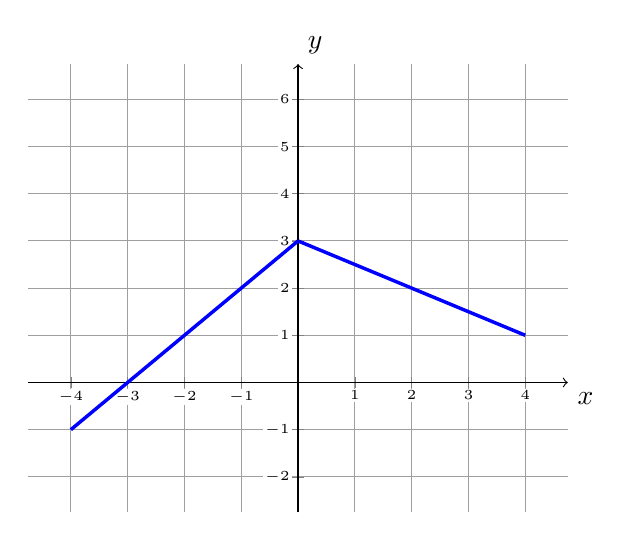
\begin{tikzpicture}[scale=1.0]
        \begin{axis}[
          grid=both,
          grid style={line width=0.35pt, draw=gray!75},
          axis lines=center,
          axis line style={->},
          xmin=-4, xmax=4,
          ymin=-2, ymax=6,
          xtick={-4,-3,...,4},
          ytick={-2,-1,...,6},
          enlargelimits={abs=0.75},
          ticklabel style={font=\tiny,inner sep=0.75pt,fill=white},
          xlabel=$x$, xlabel style={at={(ticklabel* cs:1)},anchor=north west},
          ylabel=$y$, ylabel style={at={(ticklabel* cs:1)},anchor=south west},
          ]
          \addplot[domain=-4:0,blue, line width=1.25pt] {\x+3};
          \addplot[domain=0:4,blue, line width=1.25pt] {-0.5*\x+3};
      \end{axis}
    \end{tikzpicture}\\[\stretch{0.5}]
  \end{ex*}
  \pagebreak
  (Brigs: 1.2.25, 1.2.26) Write a definition of the function whose graph is given.
  \begin{ex*}\ 
  
    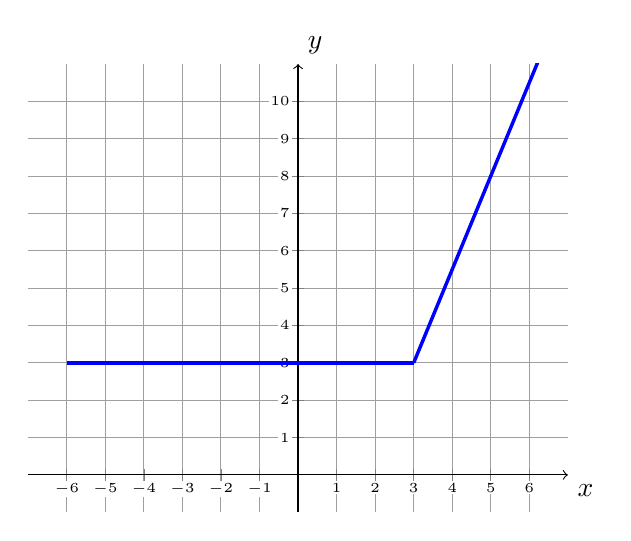
\begin{tikzpicture}[scale=1.0]
        \begin{axis}[
          grid=both,
          grid style={line width=0.35pt, draw=gray!75},
          axis lines=center,
          axis line style={->},
          xmin=-6, xmax=6,
          ymin=0, ymax=10,
          xtick={-6,-5,...,6},
          ytick={0,1,...,10},
          enlargelimits={abs=1.0},
          ticklabel style={font=\tiny,inner sep=0.75pt,fill=white},
          xlabel=$x$, xlabel style={at={(ticklabel* cs:1)},anchor=north west},
          ylabel=$y$, ylabel style={at={(ticklabel* cs:1)},anchor=south west},
          ]
          \addplot[domain=-6:3,blue, line width=1.25pt] {3};
          \addplot[domain=3:7,blue, line width=1.25pt] {5/2*\x-9/2};
      \end{axis}
    \end{tikzpicture}\\[\stretch{1}]
  \end{ex*}
  \begin{ex*}\ 
  
    \begin{tikzpicture}[scale=1.0]
        \begin{axis}[
          grid=both,
          grid style={line width=0.35pt, draw=gray!75},
          axis lines=center,
          axis line style={->},
          xmin=0, xmax=8,
          ymin=-2, ymax=6,
          xtick={-6,-5,...,8},
          ytick={-2,-1,...,10},
          enlargelimits={abs=0.5},
          ticklabel style={font=\tiny,inner sep=0.75pt,fill=white},
          xlabel=$x$, xlabel style={at={(ticklabel* cs:1)},anchor=north west},
          ylabel=$y$, ylabel style={at={(ticklabel* cs:1)},anchor=south west},
          ]
          \addplot[domain=0:3,blue, line width=1.25pt] {\x+1};
          \addplot[domain=3:8,blue, line width=1.25pt] {-\x/3+ 3};
          \addplot[holdot] coordinates{(3,4)};
          \addplot[soldot] coordinates{(3,2)};
      \end{axis}
    \end{tikzpicture}\\[\stretch{1}]
  \end{ex*}
  \pagebreak
  (Briggs: 1.2.31, 1.2.33, 1.2.34) Graph the following functions
  \begin{ex*}
    $f(x)=\left\{\begin{array}{ll}
      3x-1& \text{if } x\leq 0\\
      -2x+1& \text{if } x>0
    \end{array}
    \right.$\\[\stretch{1}]
  \end{ex*}
  \begin{ex*}
    $f(x)=\left\{\begin{array}{ll}
      -2x-1& \text{if } x\leq -1\\
      1& \text{if } -1\leq x\leq 1\\
      2x-1& \text{if } x>1
    \end{array}
    \right.$\\[\stretch{1}]
  \end{ex*}
  \begin{ex*}
    $f(x)=\left\{\begin{array}{ll}
      2x+2& \text{if } x<0\\
      x+2& \text{if } 0\leq x\leq 2      \\
      3-\frac{x}{2}& \text{if } x>2
    \end{array}
    \right.$\\[\stretch{1}]
  \end{ex*}
  \pagebreak
\end{document}

  \documentclass[../mathNotesPreamble]{subfiles}
\begin{document}
\section{JIT 4.3: Power Functions}
  \begin{defn*}
    Functions of the form $f(x)=x^r$, where $r$ is a constant, are called \textbf{power functions}.
  \end{defn*}
  \begin{enumerate}[label=]
    \item 
      \begin{minipage}{0.45\linewidth}
        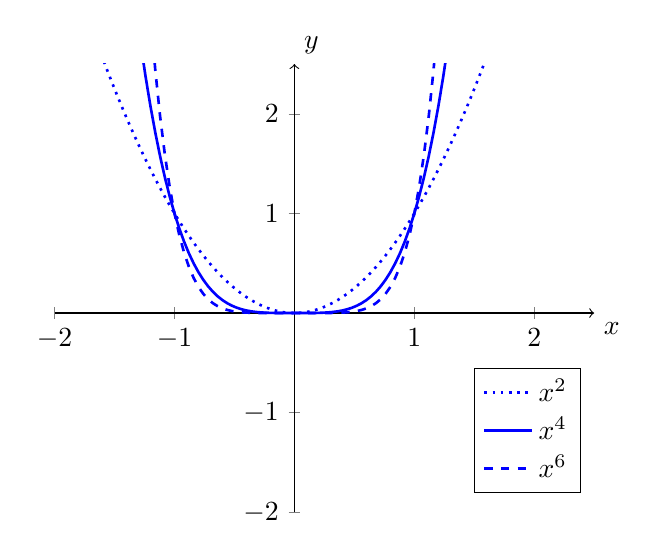
\begin{tikzpicture}[scale=1.0]
          \begin{axis}[
            axis lines=center,
            axis line style={->},
            xmin=-2, xmax=2.5,
            ymin=-2, ymax=2.5,
            xtick={-2,-1,...,2},
            ytick={-2,-1,...,2},
            xlabel=$x$, xlabel style={at={(ticklabel* cs:1)},anchor=north west},
            ylabel=$y$, ylabel style={at={(ticklabel* cs:1)},anchor=south west},
            legend style={at={(axis cs:1.5,-0.55)},anchor=north west},
            every axis plot/.append style={line width=0.95pt}
            ]
            \addplot[domain=-2:2,blue, samples = 101, dotted] {x^2};
              \addlegendentry{$x^2$};
            \addplot[domain=-2:2,blue, samples = 101] {x^4};
              \addlegendentry{$x^4$};
            \addplot[domain=-2:2,blue, samples = 101, dashed] {x^6};
              \addlegendentry{$x^6$};
          \end{axis}
        \end{tikzpicture}
      \end{minipage}%
      \begin{minipage}{0.55\linewidth}
        \begin{enumerate}[label=-]
          \item 
            These are \textbf{even} functions

            $f(-x)=f(x)$
            
          \item 
            Symmetry about the $y$-axis
            
            $(-x,y),\ (x,y)$
        \end{enumerate}
        \vspace*{100pt}
      \end{minipage}

  
      \vspace*{\stretch{1}}
    \item 
      \begin{minipage}{0.45\linewidth}
        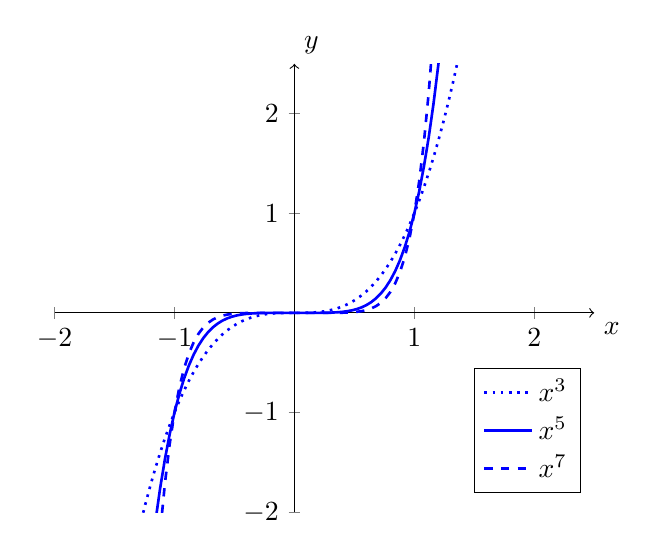
\begin{tikzpicture}[scale=1.0]
          \begin{axis}[
            axis lines=center,
            axis line style={->},
            xmin=-2, xmax=2.5,
            ymin=-2, ymax=2.5,
            xtick={-2,-1,...,2},
            ytick={-2,-1,...,2},
            xlabel=$x$, xlabel style={at={(ticklabel* cs:1)},anchor=north west},
            ylabel=$y$, ylabel style={at={(ticklabel* cs:1)},anchor=south west},
            legend style={at={(axis cs:1.5,-0.55)},anchor=north west},
            every axis plot/.append style={line width=0.95pt}
            ]
            \addplot[domain=-2:2,blue, samples = 101, dotted] {x^3};
              \addlegendentry{$x^3$};
            \addplot[domain=-2:2,blue, samples = 101] {x^5};
              \addlegendentry{$x^5$};
            \addplot[domain=-2:2,blue, samples = 101, dashed] {x^7};
              \addlegendentry{$x^7$};
          \end{axis}
        \end{tikzpicture}
      \end{minipage}%
      \begin{minipage}{0.55\linewidth}
        \begin{enumerate}[label=-]
          \item 
            These are \textbf{odd} functions

            $f(-x)=-f(x)$
          \item 
            Symmetry about the origin
            
            $(-x,-y),\ (x,y)$
        \end{enumerate}
        \vspace*{100pt}
      \end{minipage}

      \vspace*{\stretch{0.75}}
      \pagebreak
      
      \item 
      \begin{minipage}{0.5\linewidth}
        \begin{tikzpicture}[scale=1.0]
          \begin{axis}[
            axis lines=center,
            axis line style={->},
            xmin=-2, xmax=2.5,
            ymin=-1.5, ymax=1.75,
            xtick={-2,-1,...,2},
            ytick={-2,-1,...,2},
            xlabel=$x$, xlabel style={at={(ticklabel* cs:1)},anchor=north west},
            ylabel=$y$, ylabel style={at={(ticklabel* cs:1)},anchor=south west},
            legend style={at={(axis cs:1.5,-0.55)},anchor=north west},
            every axis plot/.append style={line width=0.95pt}
            ]
            \addplot[domain=0:2.5,blue, samples = 101, dotted] {x^0.5};
              \addlegendentry{$x^{\sfrac12}$};
            \addplot[domain=0:2.5,blue, samples = 101] {x^0.25};
              \addlegendentry{$x^{\sfrac14}$};
            \addplot[domain=0:2.5,blue, samples = 101, dashed] {x^0.16};
              \addlegendentry{$x^{\sfrac16}$};
          \end{axis}
        \end{tikzpicture}
      \end{minipage}%
      \begin{minipage}{0.5\linewidth}
        \begin{tikzpicture}[scale=1.0]
          \begin{axis}[
            axis lines=center,
            axis line style={->},
            xmin=-2, xmax=2.5,
            ymin=-1.5, ymax=1.75,
            xtick={-2,-1,...,2},
            ytick={-2,-1,...,2},
            xlabel=$x$, xlabel style={at={(ticklabel* cs:1)},anchor=north west},
            ylabel=$y$, ylabel style={at={(ticklabel* cs:1)},anchor=south west},
            legend style={at={(axis cs:1.5,-0.55)},anchor=north west},
            every axis plot/.append style={line width=0.9pt}
            ]
            \def\g(#1){(#1)}
            \def\f(#1,#2){(\g(#1))/abs(\g(#1))*(abs(\g(#1)))^(#2)};
            \addplot[domain=-2:2,blue, samples = 501, dotted] {\f(\x,1/3)};
              \addlegendentry{$x^{\sfrac13}$};
            \addplot[domain=-2:2,blue, samples = 501] {\f(\x,1/5)};
              \addlegendentry{$x^{\sfrac15}$};
            \addplot[domain=-2:2,blue, samples = 501, dashed] {\f(\x,1/7)};
              \addlegendentry{$x^{\sfrac17}$};
          \end{axis}
        \end{tikzpicture}
      \end{minipage}

  
      \vspace*{\stretch{1}}

      \begin{center}
        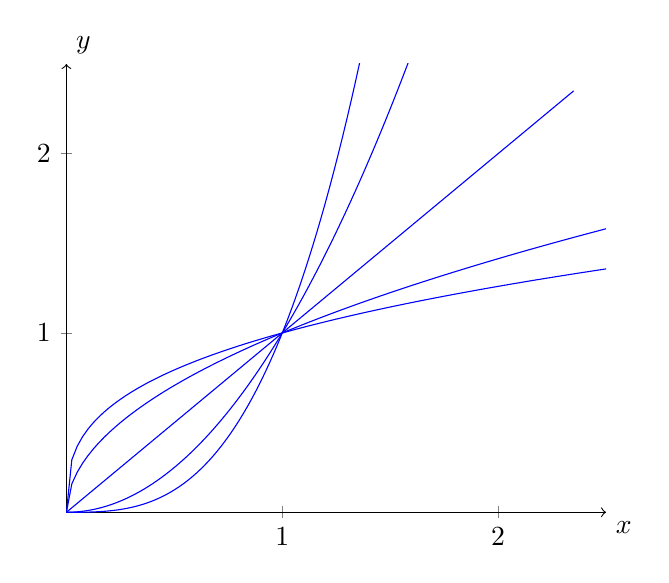
\begin{tikzpicture}[scale=1.0]
          \begin{axis}[
            axis lines=center,
            axis line style={->},
            xmin=0, xmax=2.5,
            ymin=0, ymax=2.5,
            xtick={-2,-1,...,2},
            ytick={-2,-1,...,2},
            xlabel=$x$, xlabel style={at={(ticklabel* cs:1)},anchor=north west},
            ylabel=$y$, ylabel style={at={(ticklabel* cs:1)},anchor=south west},
            legend style={at={(axis cs:1.5,-0.55)},anchor=north west},
            %every axis plot/.append style={line width=0.95pt}
            ]
            \addplot[domain=0:2.5,blue, samples = 101] {x^(1/3)};
            \addplot[domain=0:2.5,blue, samples = 101] {x^(1/2)};
            \addplot[domain=0:2.35,blue, samples = 101] {x^1};
            \addplot[domain=0:2,blue, samples = 101] {x^2};
            \addplot[domain=0:2,blue, samples = 101] {x^3};
          \end{axis}
        \end{tikzpicture}
      \end{center}

      \pagebreak      
      \item 
      \begin{minipage}{0.5\linewidth}
        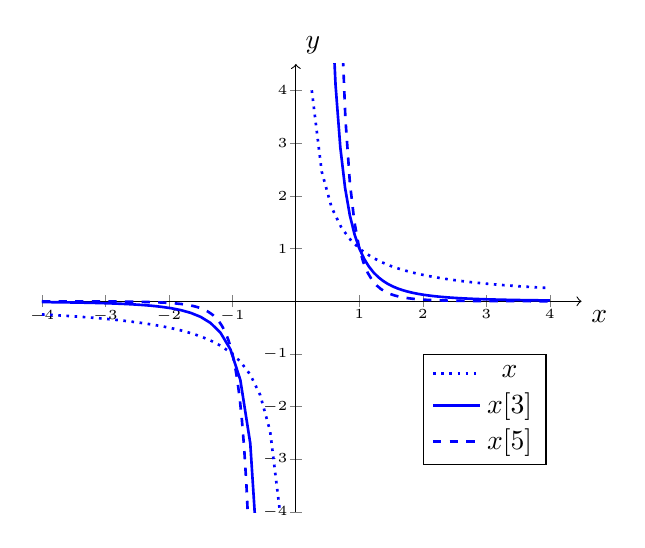
\begin{tikzpicture}[scale=1.0]
          \begin{axis}[
            axis lines=center,
            axis line style={->},
            xmin=-4, xmax=4.5,
            ymin=-4, ymax=4.5,
            xtick={-4,-3,...,4},
            ytick={-4,-3,...,4},
            ticklabel style={font=\tiny, inner sep=0.75pt},
            xlabel=$x$, xlabel style={at={(ticklabel* cs:1)},anchor=north west},
            ylabel=$y$, ylabel style={at={(ticklabel* cs:1)},anchor=south west},
            legend style={at={(axis cs:2,-1)},anchor=north west},
            every axis plot/.append style={line width=0.95pt}
            ]
            \addplot[unbounded coords=jump,domain=-4:-0.25,blue, dotted] {1/x};
              \addlegendentry{$x\inv$};
            \addplot[unbounded coords=jump,domain=-4:-0.25,blue] {1/x^3};
              \addlegendentry{$x\inv[3]$};
            \addplot[unbounded coords=jump,domain=-4:-0.5,blue, dashed, samples=101] {1/x^5};
              \addlegendentry{$x\inv[5]$};
            \addplot[unbounded coords=jump,domain=0.25:4,blue, dotted] {1/x};
            \addplot[unbounded coords=jump,domain=0.25:4,blue, samples = 51] {1/x^3};
            \addplot[unbounded coords=jump,domain=0.5:4,blue, samples = 51, dashed] {1/x^5};
          \end{axis}
        \end{tikzpicture}
      \end{minipage}%
      \begin{minipage}{0.5\linewidth}
        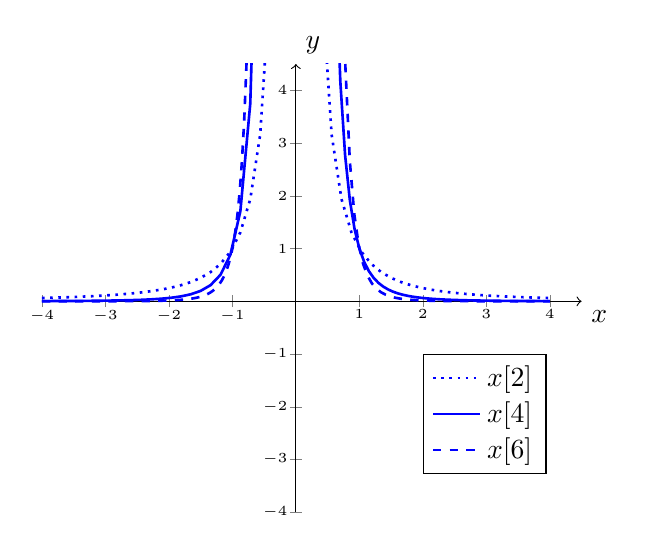
\begin{tikzpicture}[scale=1.0]
          \begin{axis}[
            axis lines=center,
            axis line style={->},
            xmin=-4, xmax=4.5,
            ymin=-4, ymax=4.5,
            xtick={-4,-3,...,4},
            ytick={-4,-3,...,4},
            ticklabel style={font=\tiny, inner sep=0.75pt},
            xlabel=$x$, xlabel style={at={(ticklabel* cs:1)},anchor=north west},
            ylabel=$y$, ylabel style={at={(ticklabel* cs:1)},anchor=south west},
            legend style={at={(axis cs:2,-1)},anchor=north west},
            every axis plot/.append style={line width=0.95pt}
            ]
            \addplot[unbounded coords=jump,domain=-4:-0.25,blue, dotted] {1/x^2};
              \addlegendentry{$x\inv[2]$};
            \addplot[unbounded coords=jump,domain=-4:-0.25,blue] {1/x^4};
              \addlegendentry{$x\inv[4]$};
            \addplot[unbounded coords=jump,domain=-4:-0.5,blue, dashed, samples=101] {1/x^6};
              \addlegendentry{$x\inv[6]$};
            \addplot[unbounded coords=jump,domain=0.25:4,blue, dotted] {1/x^2};
            \addplot[unbounded coords=jump,domain=0.25:4,blue, samples = 51] {1/x^4};
            \addplot[unbounded coords=jump,domain=0.5:4,blue, samples = 51, dashed] {1/x^6};
          \end{axis}
        \end{tikzpicture}
      \end{minipage}

      \vspace*{\stretch{1}}
      \begin{ex*}
        Determine if the following functions are symmetric about the $y$-axis, $x$-axis or the origin.
        \begin{enumerate}
          \item 
            $f(x)=3x^5+2x^3-x$\\[\stretch{0.5}]
          \item 
            $f(x)=2\abs{x}$\\[\stretch{0.5}]
          \item 
            $x^3-y^5=0$\\[\stretch{0.5}]
          \item 
            $f(x)=x\abs{x}$\\[\stretch{0.5}]
        \end{enumerate}
      \end{ex*}
    \end{enumerate}
  \pagebreak
  
\end{document}
  \documentclass[../mathNotesPreamble]{subfiles}
\begin{document}
\section{JIT 4.4: Shifting up and down}
  $$f(x)  \text{  vs. }f(x)+c$$
    \begin{minipage}{0.5\linewidth}
      \begin{center}
      \begin{tikzpicture}[scale=1.0]
        \begin{axis}[
          axis lines=center,
          axis line style={->},
          xmin=-4, xmax=4.5,
          ymin=-4, ymax=4.5,
          xtick={-4,-3,...,4},
          ytick={-4,-3,...,4},
          ticklabel style={font=\tiny, inner sep=0.75pt},
          xlabel=$x$, xlabel style={at={(ticklabel* cs:1)},anchor=north west},
          ylabel=$y$, ylabel style={at={(ticklabel* cs:1)},anchor=south west},
          legend style={at={(axis cs:2,-1)},anchor=north west},
          every axis plot/.append style={line width=0.95pt}
          ]
          \addplot[domain=-4:4,blue, samples=51, dashed] {x^2};
            \addlegendentry{$x^2$};
          \addplot[domain=-4:4,blue, samples=51] {x^2+2};
            \addlegendentry{$x^2+2$};
          \draw[->, line width = 0.9pt] (axis cs:0.75,9/16)--(axis cs:0.75,40/16);
          \draw[->, line width = 0.9pt] (axis cs:-0.75,9/16)--(axis cs:-0.75,40/16);
        \end{axis}
      \end{tikzpicture}
      \end{center}
    \end{minipage}%
    \begin{minipage}{0.5\linewidth}
      \begin{center}
      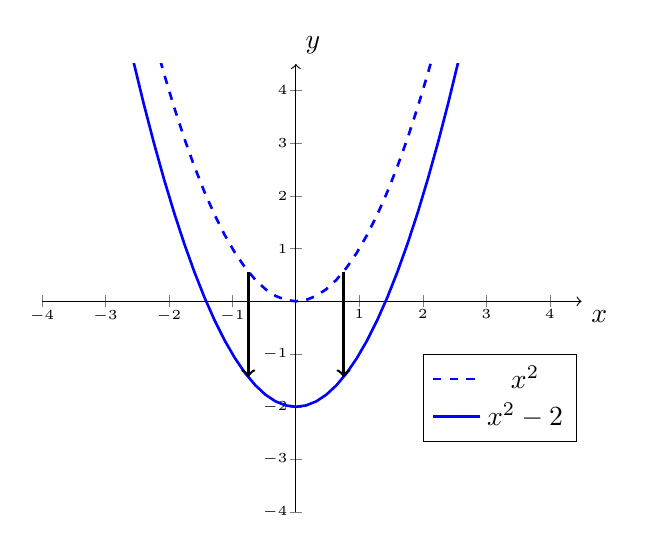
\begin{tikzpicture}[scale=1.0]
        \begin{axis}[
          axis lines=center,
          axis line style={->},
          xmin=-4, xmax=4.5,
          ymin=-4, ymax=4.5,
          xtick={-4,-3,...,4},
          ytick={-4,-3,...,4},
          ticklabel style={font=\tiny, inner sep=0.75pt},
          xlabel=$x$, xlabel style={at={(ticklabel* cs:1)},anchor=north west},
          ylabel=$y$, ylabel style={at={(ticklabel* cs:1)},anchor=south west},
          legend style={at={(axis cs:2,-1)},anchor=north west},
          every axis plot/.append style={line width=0.95pt}
          ]
          \addplot[domain=-4:4,blue, samples=51, dashed] {x^2};
            \addlegendentry{$x^2$};
          \addplot[domain=-4:4,blue, samples=51] {x^2-2};
            \addlegendentry{$x^2-2$};
          \draw[->, line width = 0.9pt] (axis cs:0.75,9/16)--(axis cs:0.75,-23/16);
          \draw[->, line width = 0.9pt] (axis cs:-0.75,9/16)--(axis cs:-0.75,-23/16);
        \end{axis}
      \end{tikzpicture}
      \end{center}
    \end{minipage}
  \vspace*{\stretch{1}}
\end{document}
  \documentclass[mathNotesPreamble]{subfiles}
\begin{document}
  \section{JIT 4.5: Shifting left and right}

    $$f(x)  \text{  vs. }f(x-c)$$
    \begin{minipage}{0.5\linewidth}
      \begin{center}
      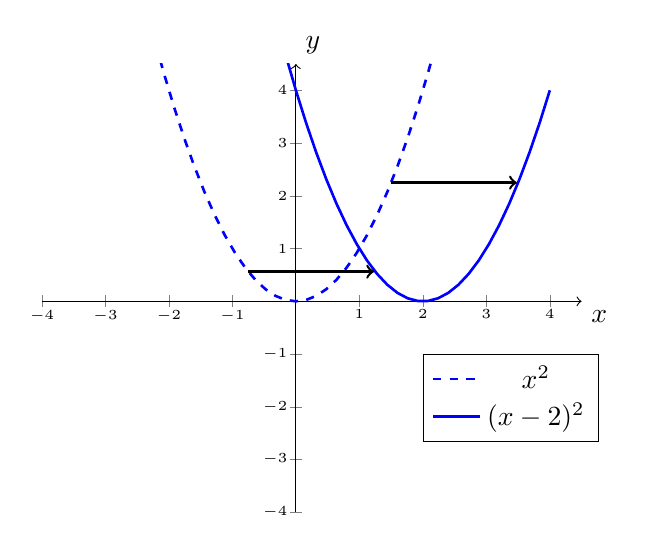
\begin{tikzpicture}[scale=1.0]
        \begin{axis}[
          axis lines=center,
          axis line style={->},
          xmin=-4, xmax=4.5,
          ymin=-4, ymax=4.5,
          xtick={-4,-3,...,4},
          ytick={-4,-3,...,4},
          ticklabel style={font=\tiny, inner sep=0.75pt},
          xlabel=$x$, xlabel style={at={(ticklabel* cs:1)},anchor=north west},
          ylabel=$y$, ylabel style={at={(ticklabel* cs:1)},anchor=south west},
          legend style={at={(axis cs:2,-1)},anchor=north west},
          every axis plot/.append style={line width=0.95pt}
          ]
          \addplot[domain=-4:4,blue, samples=51, dashed] {x^2};
            \addlegendentry{$x^2$};
          \addplot[domain=-4:4,blue, samples=51] {(x-2)^2};
            \addlegendentry{$(x-2)^2$};
          \draw[->, line width = 0.9pt] (axis cs:1.5,2.25)--(axis cs:3.48,2.25);
          \draw[->, line width = 0.9pt] (axis cs:-0.75,9/16)--(axis cs:1.23,9/16);
        \end{axis}
      \end{tikzpicture}
      \end{center}
    \end{minipage}%
    \begin{minipage}{0.5\linewidth}
      \begin{center}
      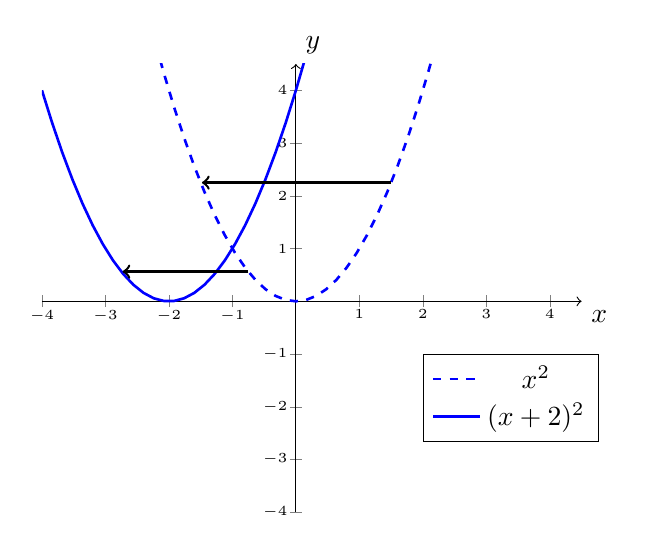
\begin{tikzpicture}[scale=1.0]
        \begin{axis}[
          axis lines=center,
          axis line style={->},
          xmin=-4, xmax=4.5,
          ymin=-4, ymax=4.5,
          xtick={-4,-3,...,4},
          ytick={-4,-3,...,4},
          ticklabel style={font=\tiny, inner sep=0.75pt},
          xlabel=$x$, xlabel style={at={(ticklabel* cs:1)},anchor=north west},
          ylabel=$y$, ylabel style={at={(ticklabel* cs:1)},anchor=south west},
          legend style={at={(axis cs:2,-1)},anchor=north west},
          every axis plot/.append style={line width=0.95pt}
          ]
          \addplot[domain=-4:4,blue, samples=51, dashed] {x^2};
            \addlegendentry{$x^2$};
          \addplot[domain=-4:4,blue, samples=51] {(x+2)^2};
            \addlegendentry{$(x+2)^2$};
          \draw[->, line width = 0.9pt] (axis cs:1.5,2.25)--(axis cs:-1.48,2.25);
          \draw[->, line width = 0.9pt] (axis cs:-0.75,9/16)--(axis cs:-2.73,9/16);
        \end{axis}
      \end{tikzpicture}
      \end{center}
    \end{minipage}
  \vspace*{\stretch{1}}
  
  \pagebreak
\end{document}
  \documentclass[answers]{exam}
\usepackage{texPreamble}
\usepackage{relsize}
\usepackage{tabularx}
\extraheadheight{0.25in}
\extrafootheight{1.0in}
\extrawidth{1in}
% ----------------------------------------------------------------

\begin{document}
%\relscale{1.4}
  \section{JIT 4.6: Translations}
    \begin{ex*}\ 
    
      \begin{minipage}{0.45\linewidth}
        Graph $\dfrac{1}{x-1}+2$
        \vspace*{100pt}
      \end{minipage}%
      \begin{minipage}{0.5\linewidth}
        \begin{center}
          \begin{tikzpicture}[scale=1.0]
            \begin{axis}[
              axis lines=center,
              axis line style={->},
              xmin=-4, xmax=4.5,
              ymin=-4, ymax=4.5,
              xtick={-4,-3,...,4},
              ytick={-4,-3,...,4},
              ticklabel style={font=\tiny,inner sep=0.75pt},
              xlabel=$x$, xlabel style={at={(ticklabel* cs:1)},anchor=north west},
              ylabel=$y$, ylabel style={at={(ticklabel* cs:1)},anchor=south west},
              legend style={at={(axis cs:2,-1)},anchor=north west},
              every axis plot/.append style={line width=0.95pt}
              ]
              \addplot[domain=-4:0.9,blue, samples=51] {1/(x-1)+2};
              \addplot[domain=1.1:4,blue, samples=51] {1/(x-1)+2};
            \end{axis}
          \end{tikzpicture}
        \end{center}
      \end{minipage}
    \end{ex*}
    \vspace*{\stretch{1}}
    \begin{ex*}\ 
    
      \begin{minipage}{0.45\linewidth}
        Graph $g(x)=x^2-6x+5$
        \vspace*{100pt}
      \end{minipage}%
      \begin{minipage}{0.5\linewidth}
        \begin{center}
          \begin{tikzpicture}[scale=1.0]
            \begin{axis}[
              axis lines=center,
              axis line style={->},
              xmin=-2, xmax=6.5,
              ymin=-5, ymax=6.5,
              xtick={-4,-3,...,7},
              ytick={-4,-3,...,7},
              ticklabel style={font=\tiny,inner sep=0.75pt},
              xlabel=$x$, xlabel style={at={(ticklabel* cs:1)},anchor=north west},
              ylabel=$y$, ylabel style={at={(ticklabel* cs:1)},anchor=south west},
              legend style={at={(axis cs:2,-1)},anchor=north west},
              every axis plot/.append style={line width=0.95pt}
              ]
              \addplot[domain=-4:7,blue, samples=101] {x^2-6*x+5};
              \addplot[soldot] coordinates{(3,-4)} node [below right, black, yshift=5pt] {(3,-4)};
            \end{axis}
          \end{tikzpicture}
        \end{center}
      \end{minipage}
    \end{ex*}
    \vspace*{\stretch{1}}
    \pagebreak
    \textbf{Scaling a graph}
      $$f(x)\text{  vs. }cf(x)\text{  vs.  }f(cx)$$
    \begin{itemize}
      \item 
        Multiplication on the outside of the function stretches the function vertically by $c$.
      \item 
        Multiplication on the inside of the function stretches the function horizontally by $1/c$.
    \end{itemize}
    
    \begin{center}
      \begin{tikzpicture}[scale=1.0]
        \begin{groupplot}[
          group style={group size=2 by 2, horizontal sep=3.5cm, vertical sep=3cm},
          axis lines=center,
          axis line style={->},
          xmin=-4, xmax=4.5,
          ymin=-4, ymax=4.5,
          xtick={-4,-3,...,7},
          ytick={-4,-3,...,7},
          ticklabel style={font=\tiny,inner sep=0.75pt},
          legend style={at={(axis cs:2,-1)},anchor=north west},
          xlabel=$x$, xlabel style={at={(ticklabel* cs:1)},anchor=north west},
          ylabel=$y$, ylabel style={at={(ticklabel* cs:1)},anchor=south west},
          every axis plot/.append style={line width=0.95pt},
          ]
        \nextgroupplot 
          \addplot[domain=-5:5, blue, samples=101, dashed] {x^2};
            \addlegendentry{$x^2$};
          \addplot[domain=-5:5, blue, samples=101] {2*x^2};
            \addlegendentry{$2x^2$};
          \draw[->, line width = 0.9pt] (axis cs:1.45,2.1025)--(axis cs:1.45,4.20);
          \draw[->, line width = 0.9pt] (axis cs:-1.45,2.1025)--(axis cs:-1.45,4.20);
        \nextgroupplot 
          \addplot[domain=-5:5, blue, samples=101, dashed] {x^2};
            \addlegendentry{$x^2$};
          \addplot[domain=-5:5, blue, samples=101] {(2*x)^2};
            \addlegendentry{$(2x)^2$};
          \draw[->, line width = 0.9pt] (axis cs:2,4)--(axis cs:1.025,4);
          \draw[->, line width = 0.9pt] (axis cs:-2,4)--(axis cs:-1.025,4);
        \nextgroupplot 
          \addplot[domain=-5:5, blue, samples=101, dashed] {x^2};
            \addlegendentry{$x^2$};
          \addplot[domain=-5:5, blue, samples=101] {0.5*x^2};
            \addlegendentry{$\frac12x^2$};
          \draw[->, line width = 0.9pt] (axis cs:2,4)--(axis cs:2,2);
          \draw[->, line width = 0.9pt] (axis cs:-2,4)--(axis cs:-2,2);
        \nextgroupplot 
          \addplot[domain=-5:5, blue, samples=101, dashed] {x^2};
            \addlegendentry{$x^2$};
          \addplot[domain=-5:5, blue, samples=101] {(0.5*x)^2};
            \addlegendentry{$\parens{\frac12x}^2$};
          \draw[->, line width = 0.9pt] (axis cs:2,4)--(axis cs:4,4);
          \draw[->, line width = 0.9pt] (axis cs:-2,4)--(axis cs:-4,4);
        \end{groupplot}
      \end{tikzpicture}
    \end{center}
    \pagebreak
    \begin{ex*}\ 
    
      \begin{minipage}{0.45\linewidth}
        Graph $f(t)=40t-5t^2$
        \vspace*{100pt}
      \end{minipage}%
      \begin{minipage}{0.5\linewidth}
        \begin{center}
          \begin{tikzpicture}[scale=1.0]
            \begin{axis}[
              axis lines=center,
              axis line style={->},
              xmin=-5, xmax=5,
              ymin=-5, ymax=5,
              xmajorticks=false,
              ymajorticks=false,
              xlabel=$x$, xlabel style={at={(ticklabel* cs:1)},anchor=north west},
              ylabel=$y$, ylabel style={at={(ticklabel* cs:1)},anchor=south west},
              ]
            \end{axis}
          \end{tikzpicture}
        \end{center}
      \end{minipage}
    \end{ex*}
    \vspace*{\stretch{1}}
    \begin{ex*}\ 
    
      \begin{minipage}{0.45\linewidth}
        Graph $g(h)=100\pi h$
        \vspace*{100pt}
      \end{minipage}%
      \begin{minipage}{0.5\linewidth}
        \begin{center}
          \begin{tikzpicture}[scale=1.0]
            \begin{axis}[
              axis lines=center,
              axis line style={->},
              xmin=-5, xmax=5,
              ymin=-5, ymax=5,
              xmajorticks=false,
              ymajorticks=false,
              xlabel=$x$, xlabel style={at={(ticklabel* cs:1)},anchor=north west},
              ylabel=$y$, ylabel style={at={(ticklabel* cs:1)},anchor=south west},
              ]
            \end{axis}
          \end{tikzpicture}
        \end{center}
      \end{minipage}
    \end{ex*}
    \vspace*{\stretch{1}}
    \pagebreak
    \section*{Composition}
    $$\parens{f\circ g}(x)=f\parens{g(x)}$$
    \begin{ex*}
      \begin{enumerate}[label=]
        \item $f(x)=\sqrt{x}$,\ \  $g(x)=x+1$
        \item $\parens{f \circ g}(x)=$
        \item $\parens{g\circ f}(x)=$
      \end{enumerate}
    \end{ex*}
    \vspace*{\stretch{1}}
\end{document}

  \documentclass[mathNotesPreamble]{subfiles}
\begin{document}
%\relscale{1.4}
    \section{JIT 4.7: Intersection of curves and simultaneous solutions}
    \begin{ex*}\ 
    
      $\begin{array}{l}
        y=x^2-4\\
        x+y=8
      \end{array}$
      \vspace*{\stretch{1}}
    \end{ex*}
    
    \pagebreak

    \begin{ex*}\ 
    
      $\begin{array}{r@{\,=\,}l}
        2x+3y&7\\
        -3x+7y&11
      \end{array}$
    \end{ex*}
    
    \vspace*{\stretch{1}}
    \begin{minipage}[t]{0.5\linewidth}
    \noindent
    \begin{ex*}\ 
    \end{ex*}
      $\begin{array}{r@{\,=\,}l}
        y&x+7\\
        y&(x-2)^2+3
      \end{array}$
    \end{minipage}%
    \begin{minipage}[t]{0.5\linewidth}\ 
      \begin{center}
          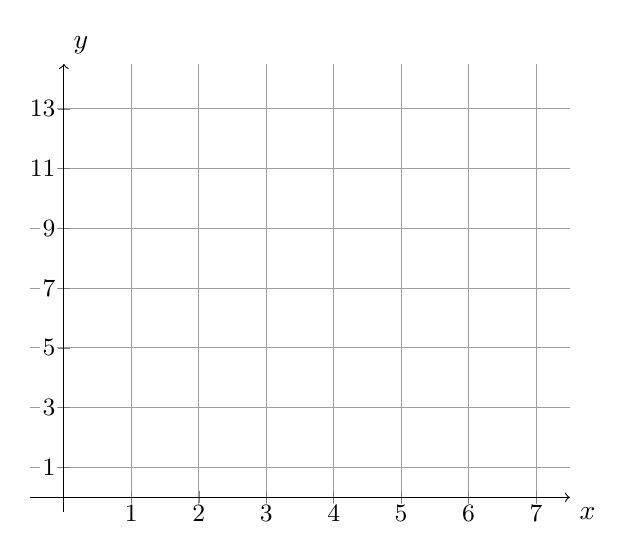
\begin{tikzpicture}[scale=1.0]
            \begin{axis}[
              axis lines=center,
              axis line style={->},
              grid=both,
              grid style={line width=0.35pt, draw=gray!75},
              xmin=-0.5, xmax=7.5,
              ymin=-0.5, ymax=14.5,
              xtick={-4,-3,...,7},
              ytick={-3,-1,...,14},
              ticklabel style={font=\small, inner sep=0.75pt, fill=white},
              xlabel=$x$, xlabel style={at={(ticklabel* cs:1)},anchor=north west},
              ylabel=$y$, ylabel style={at={(ticklabel* cs:1)},anchor=south west},
              ]
              
            \end{axis}
          \end{tikzpicture}
        \end{center}
    \end{minipage}

  \pagebreak
\end{document}

  \documentclass[../mathNotesPreamble]{subfiles}
\begin{document}
%\relsize{1.4}
  \section{JIT 5.1: Angles}
  
    \noindent
    \begin{minipage}[t]{0.6\linewidth}
      \begin{defn*}
        The \textbf{unit circle} is the circle of radius 1 that is centered at the origin.
      \end{defn*}
      \begin{defn*}
        The angle corresponding to an arc length of 1 on a unit circle is called a \textbf{radian}.
      \end{defn*}
    \end{minipage}%
    \begin{minipage}[t]{0.4\linewidth}\ 
     
      \begin{flushright}
        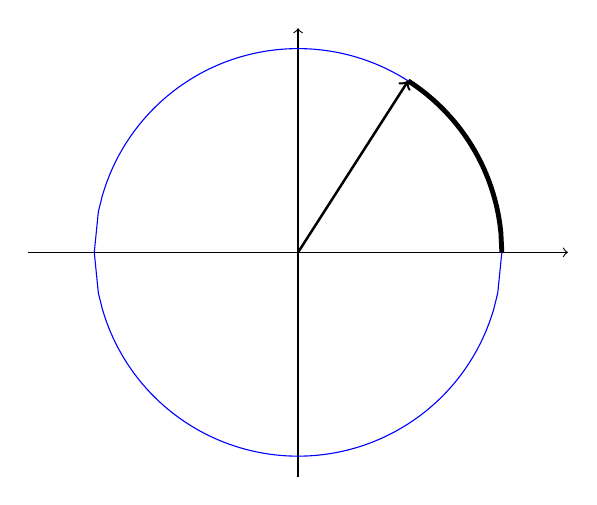
\begin{tikzpicture}[scale=1.0]
          \begin{axis}[
            axis lines=center,
            axis equal, 
            axis line style={->},
            xmin=-1.1, xmax=1.1,
            ymin=-1.1, ymax=1.1,
            xmajorticks=false,
            ymajorticks=false,
            ]
              \addplot[domain=-1:1, blue, samples=101] {sqrt(1-x^2)};
              \addplot[domain=0.5403:1, black, samples=101, line width=1.75pt] {sqrt(1-x^2)};
              \draw[->, black, line width = 0.9pt] (axis cs:0,0)--(axis cs:0.5403,0.84147);
              \addplot[domain=-1:1, blue, samples=101] {-sqrt(1-x^2)};
          \end{axis}
        \end{tikzpicture}
      \end{flushright}
    \end{minipage}
    
    A circle is $2\pi$ radians or $360^\circ$. Thus:
      $$2\pi=360^\circ \Longrightarrow 1=\dfrac{180^\circ}{\pi}=\dfrac{\pi}{180^\circ}$$
    \vspace*{\stretch{1}}

    \pagebreak
\end{document}

  \documentclass[answers]{exam}
\usepackage{texPreamble}
\usepackage{relsize}
\usepackage{tabularx}
\extraheadheight{0.25in}
\extrafootheight{1.0in}
\extrawidth{1in}
% ----------------------------------------------------------------

\begin{document}
%\relscale{1.4}
  \section{JIT 5.2: Definition of $\sin(\theta)$ and $\cos(\theta)$}
    \begin{defn*}
       The coordinates of a unit circle are given by $\parens{\cos(\theta),\sin(\theta)}$ for each $\theta$.
    \end{defn*}
    \begin{defn*}
      The $\sin(\theta)$ and $\cos(\theta)$ functions are \textbf{periodic} since these functions repeat themselves over a fixed interval
    \end{defn*}
    \begin{center}
      \begin{tikzpicture}[scale=1.0]
        \begin{groupplot}[
          group style={group size=1 by 2}, 
          axis lines=center,
          axis line style={->},
          xmin=-7, xmax=7,
          ymin=-1.25, ymax=1.25,
          xtick={-6.28318, -4.7123889, ..., 6.28318},
          xticklabels={$-2\pi$, $-\frac{3\pi}{2}$,$-\pi$, $-\frac{\pi}{2}$, ,
             $\frac{\pi}{2}$,$\pi$, $\frac{3\pi}{2}$, $2\pi$},
          height=1.5in, width=0.95\linewidth,
          ticklabel style={font=\small, inner sep=0.75pt,fill=white},
          ]
          \nextgroupplot[xlabel=$\cos(\theta)$, xlabel style={at={(ticklabel* cs:1)},anchor=north west}]
            \addplot[domain=-6.28:6.28, blue, samples=101] {cos(deg(x))};
          \nextgroupplot[xlabel=$\sin(\theta)$, xlabel style={at={(ticklabel* cs:1)},anchor=north west}]
            \addplot[domain=-6.28:6.28, blue, samples=101] {sin(deg(x))};
        \end{groupplot}
      \end{tikzpicture}
    \end{center}
    \pagebreak
    \begin{defn*}
      Alternatively, $\cos(\theta)$ and $\sin(\theta)$ can be consider the ratio of the sides of a right angle triangle.
      
      \begin{minipage}{0.5\linewidth}
        \begin{tikzpicture}
          \draw (0,0) -- (8,0) -- (8,5) -- cycle;
          \draw (7.65,0) -- (7.65,0.35) -- (8,0.35);
          \node at (1,0.275) {$\theta$};
          \node at (4, -0.5) {Adj};
          \node at (8.55, 2.5) {Opp};
          \node at (4,3) {Hyp};
        \end{tikzpicture}
      \end{minipage}%
      \begin{minipage}{0.5\linewidth}
        \begin{eqnarray*}
          \sin\theta&=\dfrac{\text{Opp}}{\text{Hyp}}\\[10pt]
          \cos\theta&=\dfrac{\text{Adj}}{\text{Hyp}}\\[10pt]
          \tan\theta&=\dfrac{\text{Opp}}{\text{Adj}}\\[10pt]
        \end{eqnarray*}
      \end{minipage}
    \end{defn*}
    \vspace*{\stretch{1}}
    \pagebreak
\end{document}

  \documentclass[answers]{exam}
\usepackage{texPreamble}
\usepackage{relsize}
\usepackage{tabularx}
\extraheadheight{0.25in}
\extrafootheight{1.0in}
\extrawidth{1in}
% ----------------------------------------------------------------

\begin{document}
    \section{JIT 5.3: Special angles $\parens{\dfrac{\pi}{4}, \dfrac{\pi}{6}, \dfrac{\pi}{3}}$}
    
    \begin{minipage}{0.5\linewidth}
      \begin{tikzpicture}
        \draw (0,0) -- (8,0) -- (4,6.928) -- cycle;
        \draw[dashed] (4,0) -- (4,6.928);
        \draw (3.65,0) -- (3.65,0.35) -- (4,0.35);
        \node at (1.5,3.75) {1};
        \node at (6.5,3.75) {1};
        \node at (4,-0.5) {1};
      \end{tikzpicture}
    \end{minipage}%
    \begin{minipage}{0.5\linewidth}
      \begin{center}
        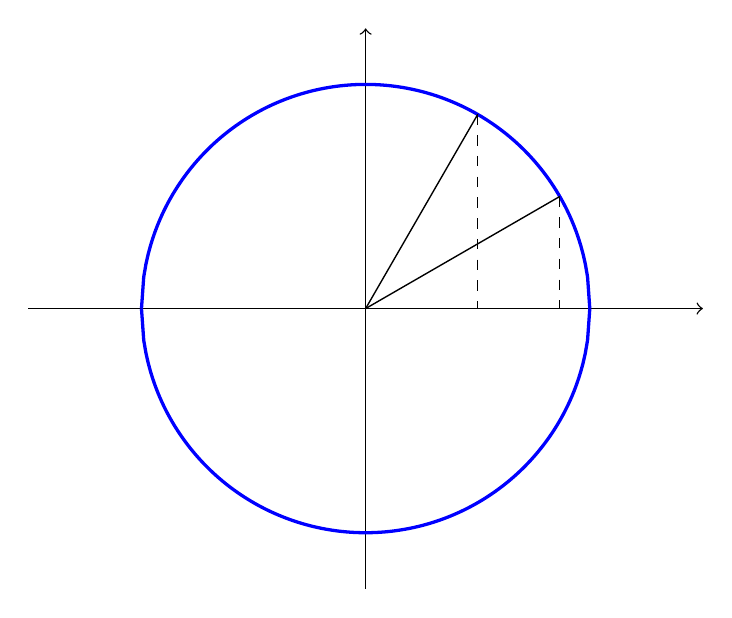
\begin{tikzpicture}[scale=1.25]
          \begin{axis}[
            axis lines=center,
            axis equal, 
            axis line style={->},
            ymin=-1.25, ymax=1.25,
            xmajorticks=false,
            ymajorticks=false,
            every axis plot/.append style={line width=0.95pt},
            ]
              \addplot[domain=-1:1, blue, samples=201] {sqrt(1-x^2)};
              \addplot[domain=-1:1, blue, samples=201] {-sqrt(1-x^2)};
              \draw (axis cs: 0,0) -- (axis cs: 0.5,0.866);
              \draw (axis cs: 0,0) -- (axis cs: 0.866,0.5);
              \draw[dashed] (axis cs: 0.866,0.5) -- (axis cs: 0.866,0);
              \draw[dashed] (axis cs: 0.5,0.866) -- (axis cs: 0.5,0);
          \end{axis}
        \end{tikzpicture}
      \end{center}
    \end{minipage}
    
    \vspace*{\stretch{1}}
    \begin{minipage}{0.475\linewidth}
      \begin{tikzpicture}[scale=0.85]
        \draw (0,0) -- (8,0) -- (8,8) -- cycle;
        \draw (7.65,0) -- (7.65,0.35) -- (8,0.35);
        \node at (4,4.5) {1};
        \node at (8.5,4) {s};
        \node at (4,-0.5) {s};
      \end{tikzpicture}
    \end{minipage}%
    \begin{minipage}{0.5\linewidth}
      \begin{center}
        \begin{tikzpicture}[scale=1.25]
          \begin{axis}[
            axis lines=center,
            axis equal, 
            axis line style={->},
            ymin=-1.25, ymax=1.25,
            xmajorticks=false,
            ymajorticks=false,
            every axis plot/.append style={line width=0.95pt},
            ]
              \addplot[domain=-1:1, blue, samples=201] {sqrt(1-x^2)};
              \addplot[domain=-1:1, blue, samples=201] {-sqrt(1-x^2)};
              \draw (axis cs: 0,0) -- (axis cs: 0.707,0.707);
              \draw[dashed] (axis cs: 0.707,0.707) -- (axis cs: 0.707,0);
          \end{axis}
        \end{tikzpicture}
      \end{center}
    \end{minipage}
    \pagebreak
    \vspace*{\stretch{0.75}}
    \begin{center}
      \newcommand{\aRad}{0.575}
      \newcommand{\rRad}{0.875}
      \newcommand{\cRad}{1.2}
      \newcommand{\lCol}{gray!90}
      \begin{tikzpicture}[scale=7.0]
        \draw[line width=1pt] (0,0) circle(1);
        \foreach \x in {0,30,...,360} {
        \draw[\lCol] (0cm,0cm) -- (\x:1);
        }
        
        \foreach \x in {45,135,225,315} {
          \draw[\lCol] (0cm,0cm) -- (\x:1);
          }
        \ifprintanswers\foreach \x/\xtext in {
          30/\dfrac{\pi}{6},
          45/\dfrac{\pi}{4},
          60/\dfrac{\pi}{3}}
          \draw (\x:\rRad) node[fill=white] {$\xtext$};
      \foreach \x/\xtext/\y in {
        30/\frac{\sqrt{3}}{2}/\frac{1}{2},
        45/\frac{\sqrt{2}}{2}/\frac{\sqrt{2}}{2},
        60/\frac{1}{2}/\frac{\sqrt{3}}{2}}
          \draw (\x:\cRad) node {$\left(\xtext,\y\right)$};
      \draw (-\cRad,0cm) node{$(-1,0)$}
            (\cRad,0cm)  node{$(1,0)$}
            (0cm,-\cRad) node{$(0,-1)$}
            (0cm,\cRad)  node{$(0,1)$};\fi
      \end{tikzpicture}
    \end{center}
    \vspace*{\stretch{1}}
    
    \pagebreak
\end{document}
  \documentclass[../mathNotesPreamble]{subfiles}
\begin{document}
    \section{JIT 5.5: The other trigonometric functions}
    $\begin{array}{r@{\ =\ }l}
      \tan\theta&\dfrac{\sin\theta}{\cos\theta}\\[15pt]
      \cot\theta&\dfrac{\cos\theta}{\sin\theta}\\[15pt]
      \sec\theta&\dfrac{1}{\cos\theta}\\[15pt]
      \csc\theta&\dfrac{1}{\sin\theta}
    \end{array}$
    
    \pagebreak
    
\end{document}
  \documentclass[mathNotesPreamble]{subfiles}
\begin{document}
%\relscale{1.4}
    \section{JIT 5.4: Graphs involving $\sin x$ and $\cos x$}
    \begin{center}
      \begin{tikzpicture}[scale=1.0]
        \begin{groupplot}[
          group style={group size=1 by 2, vertical sep=1cm},
          axis lines=center,
          axis line style={->},
          xmin=-7, xmax=7,
          ymin=-1.25, ymax=1.25,
          xtick={-6.28318, -4.7123889, ..., 6.28318},
          xticklabels={$-2\pi$, $-\frac{3\pi}{2}$,$-\pi$, $-\frac{\pi}{2}$, ,
             $\frac{\pi}{2}$,$\pi$, $\frac{3\pi}{2}$, $2\pi$},
          height=1.1in, width=0.95\linewidth,
          ticklabel style={font=\small, inner sep=0.75, fill=white},
          every axis plot/.append style={line width=0.95pt},
          ]
        \nextgroupplot[xlabel=$\cos(\theta)$, xlabel style={at={(ticklabel* cs:1)},anchor=north west}]
          \addplot[domain=-6.28:6.28, blue, samples=101] {cos(deg(x))};
        \nextgroupplot[xlabel=$\sin(\theta)$, xlabel style={at={(ticklabel* cs:1)},anchor=north west}]
          \addplot[domain=-6.28:6.28, blue, samples=101] {sin(deg(x))};
        \end{groupplot}
      \end{tikzpicture}
    \end{center}
    
    \vspace*{\stretch{1}}
    \begin{ex*}
      On $\sbrkt{0,2\pi}$, graph $\sin x$, $1+ \sin x$ and $\sin\parens{x-\dfrac{\pi}{2}}$.
      \begin{center}
        \begin{tikzpicture}
          \begin{groupplot}[
              group style={group size=1 by 2, vertical sep=50pt},
              axis lines=center,
              axis line style={->},
              xmin=0, xmax=7,
              ymin=-1.25, ymax=2.5,
              xtick={-6.28318, -4.7123889, ..., 6.28318},
              xticklabels={$-2\pi$, $-\frac{3\pi}{2}$,$-\pi$, $-\frac{\pi}{2}$, ,
                 $\frac{\pi}{2}$,$\pi$, $\frac{3\pi}{2}$, $2\pi$},
              height=2in, width=0.95\linewidth,
              ticklabel style={font=\small, inner sep=0.75, fill=white},
              every axis plot/.append style={line width=0.95pt},
              legend style={at={(axis cs:7*3.14/4,-1.25)},anchor=north west},
              ]
            \nextgroupplot[ymin=-1.25, ymax=2.5]
              \addplot[domain=0:6.28, blue, samples=101, dashed] {sin(deg(x))};
              \addlegendentry{$\sin(x)$};
              \addplot[domain=0:6.28, blue, samples=101] {1+sin(deg(x))};
              \addlegendentry{$1+\sin(x)$};
            \nextgroupplot[ymin=-1.25, ymax=1.5, height=1.95in]
              \addplot[domain=0:6.28, blue, samples=101, dashed] {sin(deg(x))};
              \addlegendentry{$\sin(x)$};
              \addplot[domain=0:6.28, blue, samples=101] {sin(deg(x-3.14/2))};
              \addlegendentry{$\sin(x-\frac{\pi}{2})$};
              \draw[->, line width = 0.95pt] (axis cs: 3.14/6, 0.5) -- (axis cs: 2*3.14/3-0.075, 0.5);
              \draw[->, line width = 0.95pt] (axis cs: 7*3.14/6, -0.5) -- (axis cs: 5*3.14/3-0.075, -0.5);
          \end{groupplot}
        \end{tikzpicture}
      \end{center}
    \end{ex*}
    \begin{defn*}
      A shift to the left or right of a wave shaped graph, such as $\sin x$ or $\cos x$, is called a \textbf{phase shift}.
    \end{defn*}
    \vspace*{\stretch{1}}
    \pagebreak

    \begin{ex*}
      Vertical scaling:
      \begin{center}
        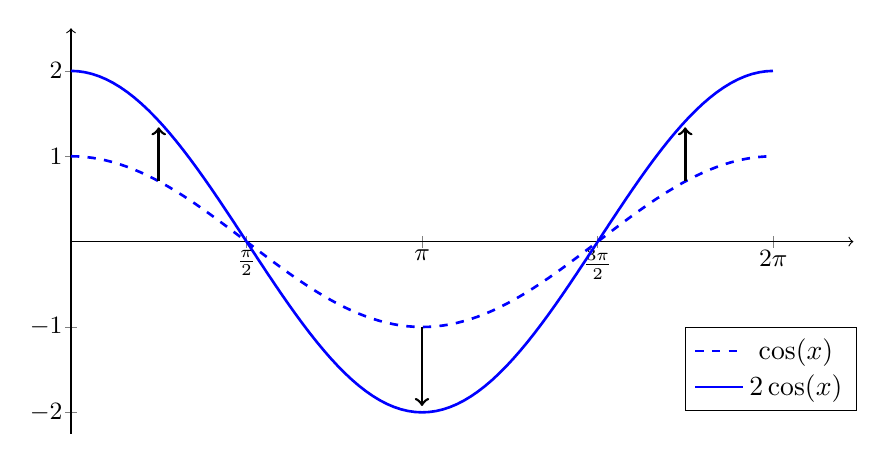
\begin{tikzpicture}
          \begin{axis}[
              axis lines=center,
              axis line style={->},
              xmin=0, xmax=7,
              ymin=-2.25, ymax=2.5,
              xtick={-6.28318, -4.7123889, ..., 6.28318},
              xticklabels={$-2\pi$, $-\frac{3\pi}{2}$,$-\pi$, $-\frac{\pi}{2}$, ,
                 $\frac{\pi}{2}$,$\pi$, $\frac{3\pi}{2}$, $2\pi$},
              ytick={-2,-1,1,2},
              height=2.65in, width=0.95\linewidth,
              ticklabel style={font=\small, inner sep=0.75, fill=white},
              legend style={at={(axis cs:7*3.14/4,-1)},anchor=north west},
              every axis plot/.append style={line width=0.95pt},
              ]
            \addplot[domain=0:6.28, blue, samples=101, dashed] {cos(deg(x))};
            \addlegendentry{$\cos(x)$};
            \addplot[domain=0:6.28, blue, samples=101] {2*cos(deg(x))};
            \addlegendentry{$2\cos(x)$};
            \draw[->, line width = 0.95pt] (axis cs: 3.14, -1) -- (axis cs: 3.14, -2+0.075);
            \draw[->, line width = 0.95pt] (axis cs: 3.14/4, 0.707) -- (axis cs: 3.14/4, 1.414-0.075);
            \draw[->, line width = 0.95pt] (axis cs: 7*3.14/4, 0.707) -- (axis cs: 7*3.14/4, 1.414-0.075);
          \end{axis}
        \end{tikzpicture}
      \end{center}
    \end{ex*}

      \begin{defn*}
        The \textbf{amplitude} of a sinusoidal graph is equal to \sfrac12 of the distance from the top to the bottom of the waves.
      \end{defn*}
      \begin{center}
        \begin{tikzpicture}
          \begin{groupplot}[
              group style={group size=1 by 2, vertical sep=55pt},
              axis lines=center,
              axis line style={->},
              xmin=0, xmax=7,
              ymin=-1.25, ymax=1.5,
              xtick={-6.28318, -4.7123889, ..., 6.28318},
              xticklabels={$-2\pi$, $-\frac{3\pi}{2}$,$-\pi$, $-\frac{\pi}{2}$, ,
                 $\frac{\pi}{2}$,$\pi$, $\frac{3\pi}{2}$, $2\pi$},
              height=2in, width=0.95\linewidth,
              ticklabel style={font=\small, inner sep=0.75, fill=white},
              legend style={at={(axis cs:7*3.14/4,-1.25)},anchor=north west},
              every axis plot/.append style={line width=0.95pt},
              ]
            \nextgroupplot
              \addplot[domain=0:6.28, blue, samples=101, dashed] {cos(deg(x))};
              \addlegendentry{$\cos(x)$};
              \addplot[domain=0:6.28, blue, samples=101] {-cos(deg(x))};
              \addlegendentry{$-\cos(x)$};
              \draw[->, line width = 0.95pt] (axis cs: 3.14, -1) -- (axis cs: 3.14, 1-0.075);
              \draw[->, line width = 0.95pt] (axis cs: 3.14/4, 0.707) -- (axis cs: 3.14/4, -0.707+0.075);
              \draw[->, line width = 0.95pt] (axis cs: 7*3.14/4, 0.707) -- (axis cs: 7*3.14/4, -0.707+0.075);
            \nextgroupplot
              \addplot[domain=0:6.28, blue, samples=101, dashed] {cos(deg(x))};
              \addlegendentry{$\cos(x)$};
              \addplot[domain=0:6.28, blue, samples=101] {0.5*cos(deg(x))};
              \addlegendentry{$\sfrac{1}{2}\cos(x)$};
              \draw[->, line width = 0.95pt] (axis cs: 3.14, -1) -- (axis cs: 3.14, -0.5-0.05);
              \draw[->, line width = 0.95pt] (axis cs: 3.14/4, 0.707) -- (axis cs: 3.14/4, 0.707/2+0.05);
              \draw[->, line width = 0.95pt] (axis cs: 7*3.14/4, 0.707) -- (axis cs: 7*3.14/4, 0.707/2+0.05);
          \end{groupplot}
        \end{tikzpicture}
      \end{center}
      \vspace*{\stretch{1}}
      \pagebreak
        
      \begin{defn*}
        \begin{itemize}
          \item The \textbf{period} of the oscillating function is the length of a cycle.
          \item For functions of the form $\sin(a x)$ the \textbf{period} is given by $\omega=\frac{2\pi}{a}$. The same holds for $\cos(a x), \sec(ax)$ and $\csc(ax)$ since these 4 functions all have a \textbf{period} of $2\pi$.
          \item When using $\tan(ax), \cot(ax)$  we need to divide $a$ by the functions original period: $\pi \Rightarrow$ \textbf{period} is $\omega=\dfrac{\pi}{a}$.
        \end{itemize}
      \end{defn*}

    \begin{center}
      \begin{tikzpicture}
        \begin{groupplot}[
            group style={group size=1 by 2, vertical sep=2cm},
            axis lines=center,
            axis line style={->},
            xmin=0, xmax=6.5,
            ymin=-1.25, ymax=1.5,
            xtick={-6.28318, -4.7123889, ..., 6.28318},
            xticklabels={$-2\pi$, $-\frac{3\pi}{2}$,$-\pi$, $-\frac{\pi}{2}$, ,
               $\frac{\pi}{2}$,$\pi$, $\frac{3\pi}{2}$, $2\pi$},
            height=2in, width=0.95\linewidth,
            ticklabel style={font=\small, inner sep=0.75, fill=white},
            legend style={at={(axis cs:7*3.14/4,-1.3)},anchor=north west},
            every axis plot/.append style={line width=0.95pt},
            ]
          \nextgroupplot
            \addplot[domain=0:6.28, blue, samples=101, dashed] {sin(deg(x))};
            \addlegendentry{$\sin(x)$};
            \addplot[domain=0:3.14, blue, samples=101] {sin(deg(2*x))};
            \addlegendentry{$\sin(2x)$};
            \draw[dashed, line width =0.95] (3.14,-1.25) -- (3.14,1.5);
            \draw[->, line width =0.95] (0,1.25) -- (3.14,1.25) node[below, pos=0.85] {$\omega=\pi$};
          \nextgroupplot[
            xmax=13, xtick={-6.28318, -4.7123889, ..., 12.566},
            xticklabels={$-2\pi$, $-\frac{3\pi}{2}$,$-\pi$, $-\frac{\pi}{2}$, ,
               $\frac{\pi}{2}$,$\pi$, $\frac{3\pi}{2}$, $2\pi$, $\frac{5\pi}{2}$,
               $3\pi$, $\frac{7\pi}{2}$, $4\pi$},
            legend style={at={(axis cs:7*3.14/2,-1.3)},anchor=north west},]
            \addplot[domain=0:6.28, blue, samples=101, dashed] {sin(deg(x))};
            \addlegendentry{$\sin(x)$};
            \addplot[domain=0:12.566, blue, samples=101] {sin(deg(0.5*x))};
            \addlegendentry{$\sin\parens{\sfrac{x}{2}}$};
            \draw[dashed, line width =0.95] (4*3.14,-1.25) -- (4*3.14,1.5);
            \draw[->, line width =0.95] (0,1.25) -- (4*3.14,1.25) node[below, pos=0.9] {$\omega=4\pi$};
        \end{groupplot}
      \end{tikzpicture}
    \end{center}
    \begin{defn*}
      The \textbf{frequency} is given by $f=\dfrac{1}{\omega}$.
    \end{defn*}
    \vspace*{\stretch{1}}
    
    \pagebreak
\end{document}
  \documentclass[mathNotesPreamble]{subfiles}
\begin{document}
    \section{JIT 15.1: Trigonometric Identities}
      \begin{defn*}
        The \textbf{Pythagorean Identity for trigonometric functions} is
          $$\sin^2(\theta)+\cos^2(\theta)=1$$
      \end{defn*}
      \pagebreak
      \begin{defn*}
        The \textbf{Angle Sum Formulas} are
        \begin{align*}
          \sin(A\pm B)&=\sin(A)\cos(B)\pm\cos(A)\sin(B)\\
          \cos(A\pm B)&=\cos(A)\cos(B)\mp\sin(A)\sin(B)
        \end{align*}
        \textbf{Note:} Since $\cos(\theta)$ is even and $\sin(\theta)$ is odd, we can derive the difference formula from the sum formula.
      \end{defn*}
      \pagebreak
      \begin{defn*}
        The \textbf{double-angle formulas} are a special case of the angle-sum formulas:
        
        \begin{minipage}{0.5\linewidth}
          \begin{align*}
            \sin(2\theta)&=\sin(\theta+\theta)\\
              &=\sin(\theta)\cos(\theta)+\cos(\theta)\sin(\theta)\\
              &=\boxed{2\sin(\theta)\cos(\theta)}
          \end{align*}
        \end{minipage}%
        \begin{minipage}{0.5\linewidth}
          \begin{align*}
            \cos(2\theta)&=\cos(\theta+\theta)\\
              &=\cos(\theta)\cos(\theta)-\sin(\theta)\sin(\theta)\\
              &=\boxed{\cos^2(\theta)-\sin^2(\theta)}
          \end{align*}
        \end{minipage}\\[15pt]
        
        \textbf{Note:} Using the Pythagorean Identity, we have 2 additional representations of $\cos(2\theta)$.
      \end{defn*}
      \pagebreak
      \begin{defn*}
        The \textbf{half-angle formulas} are derived from the double angle formula:
        \begin{align*}
          \sin(\theta)&=\pm\sqrt{\frac{1-\cos(2\theta)}{2}}\\
          \cos(\theta)&=\pm\sqrt{\frac{1+\cos(2\theta)}{2}}
        \end{align*}
      \end{defn*}
      \pagebreak
      \begin{ex*}
        Solve all the following on $\sbrkt{0,2\pi}$.
        \begin{tasks}(2)
          \task $2\theta\cos(\theta)+\theta=0$
          \task $\sin(\theta)=\frac{1}{2}$\\[2in]
          \task $4\cos^2(x)-3=0$
          \task $2\sin^2(x)-\sin(x)-1=0$\\[2in]
          \task $\sin(3x)=\dfrac{\sqrt2}{2}$
          \task $\cos(3x)=\sin(3x)$
        \end{tasks}
      \end{ex*}
      \pagebreak
\end{document}
  \documentclass[../mathNotesPreamble]{subfiles}
\begin{document}
    \section{JIT 10.1: Common Factors}
      \begin{ex*}
        Factor $3x^2y^3+15xy^4-21x^3y^2$
      \end{ex*}
      \vspace*{\stretch{0.25}}
\end{document}
  \documentclass[answers]{exam}
\usepackage{texPreamble}
\usepackage{relsize}
\usepackage{tabularx}
\extraheadheight{0.25in}
\extrafootheight{1.0in}
\extrawidth{1in}
% ----------------------------------------------------------------

\begin{document}
    \section{JIT 10.2: Special Formulas}
      \begin{enumerate}
        \item $x^2-y^2=(x+y)\cdot(x-y)$
        \item $x^3+y^3=(x+y)(x^2-xy+y^2)$
        \item $x^3-y^3=(x-y)(x^2+xy+y^2)$
        \item $x^2+2xy+y^2=(x+y)^2$
        \item $x^2-2xy+y^2=(x-y)^2$
        \item $acx^2+(bc+ad)x+bd=(ax+b)(cx+d)$
      \end{enumerate}
      \begin{ex*}
        Factor: 
        \begin{itemize}
          \item $z^2-9$\\
          \item $x^4-y^4$\\
          \item $(x-y)^2-4y^2$\\
          \item $a^3+8b^3$\\
          \item $27x^3+64y^3z^6$\\
          \item $x^2+5x+6$
        \end{itemize}
      \vspace*{\stretch{1}}
      \end{ex*}
      \pagebreak
\end{document}
  \documentclass[../mathNotesPreamble]{subfiles}
\begin{document}
\section{JIT 10.3: Grouping}
  \begin{ex*}
    Factor:
    \begin{itemize}
      \item $10xy+15y+4x+6$\\[40pt]
      \item $6x^2-11x-7$\\[40pt]
      \item $3x^2+10x+8$\\[40pt]
      \item $6ax+3ay-4bx-2by+10x+5y$\\[40pt]
    \end{itemize}
  \end{ex*}
  \pagebreak
\end{document}
  \documentclass[answers]{exam}
\usepackage{texPreamble}
\usepackage{relsize}
\usepackage{tabularx}
\extraheadheight{0.25in}
\extrafootheight{1.0in}
\extrawidth{1in}
% ----------------------------------------------------------------

\begin{document}
    \section{JIT 10.4: The Factor Theorem and Long Division}
      \begin{theorem*}[The Factor Theorem]
        Let $P(x)$ be a polynomial. Let $a$ be any real number. Then $x-a$ is a factor of $P(x)$ if and only if $P(a)=0$.
      \end{theorem*}
      \begin{ex*}
        Factor $P(x)=x^3-2x^2-5x+6$.
      \end{ex*}
      \vspace*{\stretch{1}}
      \begin{defn*}
        The \textbf{Quadratic Formula} is:
          $$x=\dfrac{-b\pm\sqrt{b^2-4ac}}{2a}$$
        where $ax^2+bx+c=0$.
      \end{defn*}
      \begin{ex*}
        Factor
        \begin{itemize}
          \item $2x^2+3x-2$\\[25pt]
          \item $x^2+x+1$\\[25pt]
        \end{itemize}
      \end{ex*}
      \pagebreak
\end{document}
  \documentclass[../mathNotesPreamble]{subfiles}
\begin{document}
    %\relscale{1.4}
    \section{JIT 2.1: Completing the Square}
      $$ax^2+bx+c=a\parens{x+\frac{b}{2a}}^2+\frac{4ac-b^2}{4a}=a\parens{x-h}^2+k$$
      \begin{center}
        \begin{tikzpicture}[scale=2.5]
          \draw[fill=ClemsonOrange] (0,0)--(1,0)--(1,1)--(0,1)--cycle;
          \draw[fill=ClemsonPurple] (1,0)--(1.5,0)--(1.5,1)--(1,1)--cycle;
          \node at (0.5,-0.125) {$x$};
          \node at (-0.125,0.5) {$x$};
          \node at (1.25,-0.125){$b$};
          \draw[->, line width=0.95] (1.55,0.5) -- (2.75,0.5);
          \draw[fill=ClemsonOrange] (3,0)--(4,0)--(4,1)--(3,1)--cycle;
          \draw[fill=ClemsonPurple] (4,0)--(4.25,0)--(4.25,1)--(4,1)--cycle;
          \draw[fill=ClemsonPurple] (3,1)--(3,1.25)--(4,1.25)--(4,1)--cycle;
          \draw[dashed, pattern=north west lines, pattern color=ClemsonPurple] (4,1.25)--(4.25,1.25)--(4.25,1)--(4,1)--cycle;
          \node at (3.5,-0.125) {$x$};
          \node at (2.875,0.5) {$x$};
          \node at (4.125,-0.15){$\frac{b}{2}$};
          \node at (2.875,1.125){$\frac{b}{2}$};
        \end{tikzpicture}
      \end{center}
      \begin{ex*}
      Complete the square for $f(x)=x^2-3x+4$
      \end{ex*}
      \vspace*{\stretch{1}}
      \begin{ex*}
      Complete the square for $f(x)=4x^2+20x-100$
      \end{ex*}
      \vspace*{\stretch{1}}
      \pagebreak
      \begin{defn*}
        The equation of a circle centered at $(h,k)$ with radius $r$ is given by
          $$(x-h)^2+(y-k)^2=r^2$$
      \end{defn*}
       \begin{ex*}
        Identify the center and radius of 
          $$x^2-2x+y^2+2y=2$$
          \vspace*{\stretch{1}}
      \end{ex*}
      \pagebreak
\end{document}

  \documentclass[../mathNotesPreamble]{subfiles}
\begin{document}
    \section{JIT 10.5: Rationalizing Numerators or Denominators Using Conjugates}
      \begin{defn*}
        A \textbf{conjugate} is formed by changing the sign between two terms in a binomial.
      \end{defn*}
      \begin{ex*}
        Rationalize the denominator of $\dfrac{x^2-3}{x+\sqrt3}$.
      \end{ex*}
      \vspace*{\stretch{1}}
      \begin{ex*}
        Write $\dfrac{1}{\sqrt{x+h}}-\dfrac{1}{\sqrt x}$ as one fraction, and rationalize the resulting numerator.
      \end{ex*}
      \vspace*{\stretch{1}}
      \pagebreak
\end{document}

  \documentclass[mathNotesPreamble]{subfiles}
\begin{document}
    \section{JIT 10.6: Extracting Factors from Radicals}
      \begin{ex*}
        Simplify $\sqrt[3]{250x^4y^3}$
      \end{ex*}
      \vspace*{\stretch{1}}
      \begin{ex*}
        Simplify $\sqrt{x^2y^6+3x^5y^4}$
      \end{ex*}
      \vspace*{\stretch{1}}
      \pagebreak
\end{document}
  \documentclass[mathNotesPreamble]{subfiles}
\begin{document}
    \section{JIT 3.1: Equations of Degree 1 (Linear equations)}
      \begin{defn*}
        The expression $ax+b$, with $a \neq 0$, is a polynomial of degree 1, and so the equation $ax + b=0$ is called an \textbf{equation of degree 1}. Since the graph of the function $ax +b$ is a straight line, the equation $ax+b=0$ is also called a \textbf{linear equation}.
      \end{defn*}
      \vspace*{25pt}
      \begin{ex*}
        Solve for $x: \hspace*{50pt} 2x+5y=3x+y+1$
      \end{ex*}
      \vspace*{\stretch{1}}
      \begin{ex*}
        Solve for $y: \hspace*{50pt} \dfrac{2}{3}y+2x-1=\dfrac{3}{4}y+x-\dfrac{1}{2}$
      \end{ex*}
      \vspace*{\stretch{1}}
      \pagebreak
\end{document}
  \documentclass[answers]{exam}
\usepackage{texPreamble}
\usepackage{relsize}
\usepackage{tabularx}
\extraheadheight{0.25in}
\extrafootheight{1.0in}
\extrawidth{1in}
% ----------------------------------------------------------------

\begin{document}
    \section{JIT 3.2: Equations of Degree 2 (Quadratic equations)}
      \begin{defn*}
        The expression $ax^2+bx+c$ with $a\neq0$ is a polynomial of degree 2, and the equation $ax^2+bx+c=0$ is called an \textbf{equation of degree 2} or a \textbf{quadratic equation}. The roots of a \textbf{quadratic equation} can be found using the \textbf{quadratic formula}:
          $$x=\dfrac{-b\pm\sqrt{b^2-4ac}}{2a}$$
      \end{defn*}
      %\vspace*{25pt}
      \begin{ex*}
        Solve for $s:\hspace*{50pt} s^2+4s+4=0$.
        \vspace*{\stretch{1}}
      \end{ex*}
      \begin{defn*}
        In the quadratic formula, if $b-4ac<0$ (called the \textbf{discriminant}), then the equation contains no Real roots. If we define $i=\sqrt{-1}$, which is an \textbf{imaginary number}, then we have a root that's a \textbf{complex number}, $a+bi$.
      \end{defn*}
      \begin{ex*}
        Solve for $y: \hspace*{50pt}y^2+2y+2=0$.
        \vspace*{\stretch{1}}
      \end{ex*}
      \pagebreak
\end{document}
  \documentclass[../mathNotesPreamble]{subfiles}
\begin{document}
    \section{JIT 3.3: Solving Other Types of Equations}
      \begin{ex*}
        Solve for $x:\hspace*{\stretch{1}} \dfrac{1}{x-5}+\dfrac{1}{x+5}=\dfrac{10}{x^2-25}.\hspace*{\stretch{1}}$ Does this root work? 
        \vspace*{\stretch{1}}
      \end{ex*}
      \begin{ex*}
        Solve for $x:\hspace*{50pt} x^4-5x^2-36=0$ \hspace*{\stretch{1}}\textit{Hint:} Let $y=x^2$.
        \vspace*{\stretch{1}}
      \end{ex*}
      \pagebreak
      \begin{ex*}
        Solve for $x:\hspace*{50pt} x^6+6x^3-16=0$
        \vspace*{\stretch{1}}
      \end{ex*}
      \begin{ex*}
        Solve for $x:\hspace*{50pt} x+\sqrt x-6=0$
        \vspace*{\stretch{1}}
      \end{ex*}
      \pagebreak
\end{document}
  \documentclass[answers]{exam}
\usepackage{texPreamble}
\usepackage{relsize}
\usepackage{tabularx}
\extraheadheight{0.25in}
\extrafootheight{1.0in}
\extrawidth{1in}
% ----------------------------------------------------------------

\begin{document}
  \section{2.1: The Idea of Limits}
    \begin{defn*}
      The \textbf{average velocity} is the distance traveled over some time period.
      
      The \textbf{instantaneous velocity} is the limit of the average velocities as the length of the time period goes to zero.
    \end{defn*}
    \begin{ex*}
      An unladen swallow is flying from Camelot to the Castle Anthrax and back. It's current position, in miles, is given by
        $$s(t)=-16t^2+96t$$
      where $t$ is given in hours. Find the average velocity between:
      \begin{tasks}(2)
        \task $t=1$ and $t=3$,
        \task $t=1$ and $t=2$,
      \end{tasks}
    \end{ex*}
    \vspace*{\stretch{1}}
    \begin{ex*}
      Find the instantaneous velocity using $s(t)$ by computing the average velocity between $t=1$ and $t=h$:
    \end{ex*}
    %\vspace*{\stretch{1}}
    \begin{flushright}
      \begin{tikzpicture}
        \begin{axis}[
          axis lines=center,
          axis line style={->},
          x=2.5cm,
          xmin=-0.25, xmax=3.5,
          ymin=-10, ymax=175,
          xtick={0,1,2,3},
          ytick={50,100,150},
          xlabel=$t$, xlabel style={at={(ticklabel* cs:1)},anchor=north west},
          ylabel=$s(t)$, ylabel style={at={(ticklabel* cs:1)},anchor=south west},
          every axis plot/.append style={line width=0.95pt}
          ]
          \addplot[->] expression[domain=0:3.5] {-16*x^2+96*x};
          \addplot[soldot] coordinates{(1,80)}  node[below right, black] {$(1,80)$};
          \addplot[soldot] coordinates{(2,128)} node[above left, black] {$(2,128)$};
          \addplot[soldot] coordinates{(3,144)} node[below, black, xshift=5pt, yshift=-5pt] {$(3,144)$};
          \addplot[domain=0.5:3.25] {48*x+32};
          \addplot[domain=0.5:3.25] {32*x+48};
        \end{axis}
      \end{tikzpicture}
      \vspace*{-30pt}
    \end{flushright}
    \pagebreak
    \begin{defn*}
      The \textbf{secant line} is the line that intersects the function in two places. 
       
       The \textbf{tangent line} is the line that intersects the function in exactly one place (locally).
    \end{defn*}
    \textit{Note--} The average velocity is the slope of the secant line. The instantaneous velocity is the slope of the tangent line. 
    \vspace*{15pt}
     \noindent
    \begin{minipage}[t]{0.55\linewidth}
      \begin{ex*}
        Using the average velocity between $t=1$ and $t=h$:
          $$v_{avg}=-16(h-5)$$
        compute the instantaneous velocity at $h=1$.
      \end{ex*}
    \end{minipage}
    \begin{minipage}[t]{0.45\linewidth}
      \begin{flushright}
        \vspace*{-15pt}
        \begin{tikzpicture}
          \begin{axis}[
            axis lines=center,
            axis line style={->},
            xmin=0.75, xmax=2.25,
            ymin=60, ymax=160,
            xtick={0,0.5,...,2},
            ytick={50,100,150},
            xlabel=$t$, xlabel style={at={(ticklabel* cs:1)},anchor=north west},
            ylabel=$s(t)$, ylabel style={at={(ticklabel* cs:1)},anchor=south west},
            every axis plot/.append style={line width=0.95pt},
            height=1.025\linewidth, 
            width=\linewidth
            ]
            \addplot[->] expression[domain=0:2.25] {-16*x^2+96*x};
            \addplot[soldot] coordinates{(1,80)}  node[below, black, yshift=-4pt, xshift=5pt] {\small $(1,80)$};
            \addplot[soldot] coordinates{(1.1,86.24)} node[below right, black, xshift=2pt, yshift=5pt] {\small $(1.1,86.24)$};
            \addplot[soldot] coordinates{(1.5,108)} node[below right, black, xshift=4pt, yshift=5pt] {\small $(1.5,108)$};
            \addplot[soldot] coordinates{(2,128)} node[below right, black, xshift=-10.5pt] {\small $(2,128)$};
            
            \addplot[domain=0.8:2.2, blue!75, fill opacity=0.5] {48*x+80-48};
            \addplot[domain=0.8:2.2, ClemsonOrange] {56*x+80-56};
            \addplot[domain=0.8:2.2, ClemsonPurple] {62.4*x+80-62.4};
          \end{axis}
        \end{tikzpicture}
      \end{flushright}
    \end{minipage}
    \begin{ex*}
      Find the instantaneous velocity of
        $$f(x)=2x^2-4x+1$$
      for any value of $x$.
    \end{ex*}
    \vspace*{\stretch{1}}
    \pagebreak
\end{document}

  \documentclass[answers]{exam}
\usepackage{texPreamble}
\usepackage{relsize}
\usepackage{tabularx}
\extraheadheight{0.25in}
\extrafootheight{1.0in}
\extrawidth{1in}
% ----------------------------------------------------------------

\begin{document}
%\relscale{1.4}
  \section{2.2: Definitions of Limits}
    \begin{defn*}(Briggs)
      Suppose the function $f$ is defined for all $x$ near $a$ except possibly at $a$. If $f(x)$ is arbitrarily close to $L$ (as close to $L$ as we like) for all $x$ sufficiently close (but not equal) to $a$, we write
        $$\lim_{x\to a} f(x)=L$$
      and say the limit of $f(x)$ as $x$ approaches $a$ equals $L$.
    \end{defn*}
    \textit{Note--} Most of the time, we can think of the limit as the value of the function if it could be evaluated at a specific point.
    \vspace*{\stretch{1}}
      
    \begin{ex*}
      Using the graph of $f$, determine the following values:\\[\stretch{1}]

      \noindent
      \begin{minipage}[b]{0.55\linewidth}
        \begin{itemize}
          \item $f(1)$ and $\ds\lim_{x\to 1}f(x)$\\[0.8in]
          \item $f(2)$ and $\ds\lim_{x\to 2}f(x)$\\[0.8in]
          \item $f(3)$ and $\ds\lim_{x\to 3}f(x)$\\[0.8in]
        \end{itemize}
      \end{minipage}%
      \begin{minipage}[b]{0.45\linewidth}
        \strut\vspace*{-\baselineskip}\newline
        \begin{flushright}
          \begin{tikzpicture}
            \begin{axis}[
              grid=both,
              grid style={line width=0.35pt, draw=gray!75},
              axis lines=center,
              axis line style={->},
              xmin=-1, xmax=6.5,
              ymin=-1, ymax=6.5,
              xtick={0,1,...,6},
              ytick={0,1,...,6},
              ticklabel style={fill=white},
              xlabel=$x$, xlabel style={at={(ticklabel* cs:1)},anchor=north west},
              ylabel=$f(x)$, ylabel style={at={(ticklabel* cs:1)},anchor=south west},
              every axis plot/.append style={line width=0.95pt}
              ]
              \addplot[<->] expression[domain=0:6.25, samples=250] {(x-2)/abs(x-2)*abs(x-2)^(1/3)+3};
              \addplot[holdot] coordinates{(2,3)(3,4)};
              \addplot[soldot] coordinates{(2,5)};
            \end{axis}
          \end{tikzpicture}
        \end{flushright}
      \end{minipage}
    \end{ex*}
    \pagebreak
      
      \begin{defn*}(Briggs)
        \def\currentname{2.2 Definitions of Limits}
        \begin{enumerate}
          \item \textbf{Right-sided limit} Suppose $f$ is defined for all $x$ near $a$ with $x>a$. If $f(x)$ is arbitrarily close to $L$ for all $x$ sufficiently close to $a$ with $x>a$, we write
            $$\lim_{x\to a^+}f(x)=L$$
          and say the limit of $f(x)$ as $x$ approaches $a$ from the right equals $L$.
          \item \textbf{Left-sided limit} Suppose $f$ is defined for all $x$ near $a$ with $x<a$. If $f(x)$ is arbitrarily close to $L$ for all $x$ sufficiently close to $a$ with $x<a$, we write
            $$\lim_{x\to a^-}f(x)=L$$
          and say the limit of $f(x)$ as $x$ approaches $a$ from the left equals $L$.
        \end{enumerate}
      \end{defn*}
      
      \vspace*{\stretch{1}}
      \noindent
        \begin{minipage}[b]{0.5\linewidth}
          \begin{ex*}
            For $f(x)=\dfrac{x^3-8}{4(x-2)}$, find
            \begin{itemize}
              \item $\ds\lim_{x\to2^+}f(x)$\\[0.95in]
              \item $\ds\lim_{x\to2^-}f(x)$\\[0.95in]
            \end{itemize}
          \end{ex*}
        \end{minipage}%
        \begin{minipage}[b]{0.5\linewidth}
        \strut\vspace*{-\baselineskip}\newline
          \begin{flushright}
            \begin{tikzpicture}
              \begin{axis}[
                axis lines=center,
                axis line style={->},
                xmin=-0.5, xmax=3.5,
                ymin=-0.6, ymax=4.5,
                xtick={0,1,...,3},
                ytick={0,1,...,8},
                ticklabel style={fill=white},
                xlabel=$x$, xlabel style={at={(ticklabel* cs:1)},anchor=north west},
                ylabel=$f(x)$, ylabel style={at={(ticklabel* cs:1)},anchor=south west},
                every axis plot/.append style={line width=0.95pt}
              ]
              \addplot[<->] expression[domain=-0.5:2.75] {(x^2+2*x+4)/4};
              \addplot[holdot] coordinates{(2,3)};
              \end{axis}
            \end{tikzpicture}
          \end{flushright}
        \end{minipage}%
      
      \pagebreak
      
      \begin{defn*}(Briggs)
        \textbf{Relationship Between One-Sided and Two-Sided Limits}
        
        Assume $f$ is defined for all $x$ near $a$ except possibly at $a$. Then $\ds\lim_{x\to a}f(x)=L$ if and only if $\ds\lim_{x\to a^+}f(x)=L$ and $\ds\lim_{x\to a^-} f(x)=L$. 
      \end{defn*}
      \begin{ex*}
        For $f(x)$ above, is $\ds\lim_{x\to2}f(x)$ defined? If so, what is it? What is $f(2)$?
      \end{ex*}
      \vspace*{\stretch{1}}
      \noindent 
      \begin{minipage}[b]{0.55\linewidth}
        \begin{ex*}
          Consider the graph of 
          \begin{align*}
            g(x)&=\dfrac{2x^2-6x+4}{\abs{x-1}}
              =\begin{cases}
              -2(x-2)& x<1\\
              2(x-2)& x>1
            \end{cases}
          \end{align*}
          Find
          \begin{itemize}
            \item $\ds\lim_{x\to1^-}g(x)$\\[0.5in]
            \item $\ds\lim_{x\to1^+}g(x)$\\[0.5in]
            \item $\ds\lim_{x\to1}g(x)$\\[0.5in]
          \end{itemize}
        \end{ex*}
      \end{minipage}%
      \begin{minipage}[b]{0.45\linewidth}
      \strut\vspace*{-\baselineskip}\newline
        \begin{flushright}
          \begin{tikzpicture}
            \begin{axis}[
              axis lines=center,
              axis line style={->},
              xmin=-0.5, xmax=3.5,
              ymin=-2.5, ymax=4.5,
              xtick={0,1,...,3},
              ytick={-2,-1,...,4},
              ticklabel style={fill=white},
              xlabel=$x$, xlabel style={at={(ticklabel* cs:1)},anchor=north west},
              ylabel=$g(x)$, ylabel style={at={(ticklabel* cs:1)},anchor=south west},
              every axis plot/.append style={line width=0.95pt}
              ]
              \addplot[<-] expression[domain=-0.25:1, blue] {-2*(x-2)};
              \addplot[->] expression[domain=1:3.25, blue] {2*(x-2)};
              \addplot[holdot] coordinates{(1,2)(1,-2)};
            \end{axis}
          \end{tikzpicture}
        \end{flushright}
      \end{minipage}
      \pagebreak
      
      \begin{ex*}
        Consider the function
          $$h(x)=\frac{x^2-81}{2x+18}$$
        What does this function look like? What is $h(-9)$? What is $\ds\lim_{x\to-9} h(x)$?
      \end{ex*}
      \vspace*{\stretch{1}}
      \noindent 
      \begin{minipage}[t]{0.6\linewidth}\ 
        \begin{ex*}
          The ceiling function is 
            $$j(x)=\ceil{x}$$
          where $\ceil{x}$ returns the smallest integer greater than or equal to $x$. In other words, the ceiling function always rounds up. Find the following: %(What do you think the floor function does?)
        \end{ex*}
      \end{minipage}%
      \begin{minipage}[t]{0.4\linewidth}\ 
        \begin{flushright}
          \begin{tikzpicture}
            \begin{axis}[
              axis equal,
              axis lines=center,
              axis line style={->},
              xmin=-2.25, xmax=3.25,
              ymin=-2.25, ymax=3.25,
              xtick={-3,-2,...,3},
              ytick={-2,-1,...,4},
              ticklabel style={fill=white},
              every axis plot/.append style={line width=0.95pt}
              ]
              \addplot[blue, domain=-2.5:3, jump mark mid] {ceil(x)};
              \addplot[holdot] coordinates{(-2,-1)(-1,0)(0,1)(1,2)(2,3)};
              \addplot[soldot] coordinates{(-2,-2)(-1,-1)(0,0)(1,1)(2,2)(3,3)};
            \end{axis}
          \end{tikzpicture}
        \end{flushright}
      \end{minipage}
      \begin{minipage}{11.5pt}
        \ 
      \end{minipage}%
      \vspace*{\stretch{0.1}}
      \begin{tasks}[after-item-skip=0.5\baselineskip, label=](4)
        \task[] $\ds\lim_{x\to 1^-} j(x)$ 
        \task[] $\ds\lim_{x\to 1^+} j(x)$ 
        \task[] $\ds\lim_{x\to 1} j(x)$ 
        \task[] $j(1)$
        \task[] $\ds\lim_{x\to 1.5^-} j(x)$ 
        \task[] $\ds\lim_{x\to 1.5^+} j(x)$ 
        \task[] $\ds\lim_{x\to 1.5} j(x)$ 
        \task[] $j(1.5)$ 
      \end{tasks}
      \vspace*{\stretch{0.1}}
      \pagebreak
      \begin{ex*}
        Consider the function
          $$h(x)=\cos\parens{\frac{1}{x}}$$
        What is $\ds\lim_{x\to0} h(x)$?
        
        \begin{minipage}{0.6\linewidth}
          Consider $x=1/(n\pi)$. As $n\to\infty, x\to0$, then,
            $$\cos\parens{\frac{1}{x}}=\cos\parens{n\pi}=
            \begin{cases}
              1& \text{if } n\text{ is even}\\
              -1& \text{if } n\text{ is odd}
            \end{cases}$$
        \end{minipage}%
        \begin{minipage}{0.4\linewidth}
          \begin{flushright}
            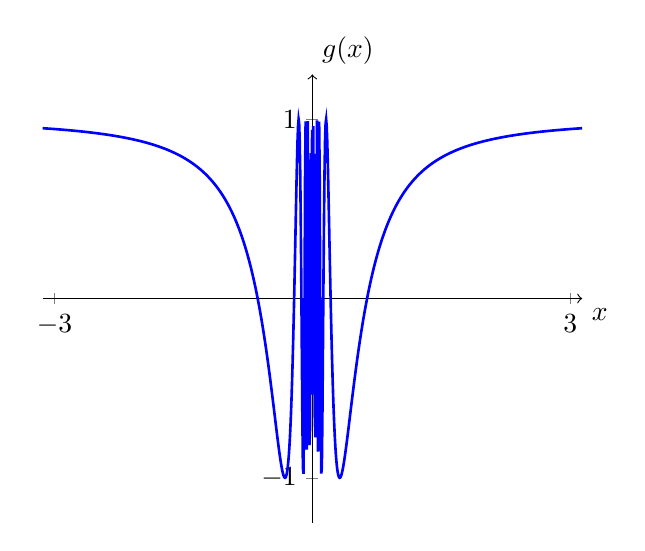
\begin{tikzpicture}
              \begin{axis}[
                axis lines=center,
                axis line style={->},
                xmin=-3.14, xmax=3.14,
                ymin=-1.25, ymax=1.25,
                xtick={-3,3},
                ytick={-1,1},
                ticklabel style={fill=white},
                xlabel=$x$, xlabel style={at={(ticklabel* cs:1)},anchor=north west},
                ylabel=$g(x)$, ylabel style={at={(ticklabel* cs:1)},anchor=south west},                every axis plot/.append style={line width=0.95pt}
                ]
              \addplot[-] expression[domain=-3.14:3.14, samples=1000, blue] {cos(deg 1/x)};
              \end{axis}
            \end{tikzpicture}
          \end{flushright}
        \end{minipage}
      \end{ex*}
      \vspace*{\stretch{1}}
      \begin{ex*}
        Graph an example with the following characteristics:
          $$\lim_{x\to-2^-} f(x)=-4\qquad 
            \lim_{x\to-2^+} f(x)= 2\qquad
            f(-2)=0\qquad$$
          $$\lim_{x\to4} f(x) = 2\qquad
            f(4) \textbf{ DNE}$$
          $$\lim_{x\to8} f(x) =-2\qquad
            f(8)=-2
            $$
        \begin{center}
          \begin{tikzpicture}
            \begin{axis}[
              axis lines=center,
              axis line style={->},
              height=2in, width=8in,
              xmin=-10, xmax=10,
              ymin=-6, ymax=6,
              xtick={-10,-8,...,10},
              ytick={-5,5},
              ticklabel style={fill=white},
              enlargelimits={abs=0.75},
              ]
            \end{axis}
          \end{tikzpicture}
        \end{center}
      \end{ex*}
      \pagebreak
\end{document}

  \documentclass[answers]{exam}
\usepackage{texPreamble}
\usepackage{relsize}
\usepackage{tabularx}
\extraheadheight{0.25in}
\extrafootheight{1.0in}
\extrawidth{1in}
% ----------------------------------------------------------------

\begin{document}
  \section{2.3: Techniques for Computing Limits}
    \begin{ex*}\ 
    
      \begin{tasks}(2)
        \task $\ds\lim_{x\to 3} \frac{1}{2}x-7$
        \task $\ds\lim_{x\to 2} 6$
      \end{tasks}
      \vspace*{\stretch{1}}
    \end{ex*}
    \begin{defn*}[Briggs]
      \textbf{Limit Laws:} Assume $\ds\lim_{x\to a} f(x)$ and $\ds\lim_{x\to a} g(x)$ exist. The following properties hold, where $c$ is a real number, and $n>0$ is an integer.
      
    \begin{center}
      \def\arraystretch{2.5}
      \begin{tabular}{llL}
        1.&\textbf{Sum:}
          &\ds\lim_{x\to a}\parens{f(x)+g(x)}=\lim_{x\to a}f(x)+\lim_{x\to a}g(x)\\
        2.&\textbf{Difference:}
          &\ds\lim_{x\to a}\parens{f(x)-g(x)}=\lim_{x\to a}f(x)-\lim_{x\to a}g(x)\\
        3.&\textbf{Constant multiple:}
          &\ds\lim_{x\to a}{cf(x)}=c\lim_{x\to a}f(x)\\
        4.&\textbf{Product:}
          &\ds\lim_{x\to a}{f(x)g(x)}=\parens{\lim_{x\to a}f(x)}\parens{\lim_{x\to a}g(x)}\\
        5.&\textbf{Quotient:}
          &\ds\lim_{x\to a}{\frac{f(x)}{g(x)}}=\frac{\lim_{x\to a}f(x)}{\lim_{x\to a}g(x)}, \text{ provided} \lim_{x\to a} g(x)\neq 0\\
        6.&\textbf{Power:}
          &\lim_{x\to a}\parens{f(x)}^n=\parens{\lim_{x\to a}f(x)}^n\\
        7.&\textbf{Root:}
          & \lim_{x\to a}\parens{f(x)}^{\sfrac{1}{n}}=\parens{\lim_{x\to a} f(x)}^{\sfrac{1}{n}}
       \end{tabular}
     \end{center}
    \end{defn*}
    \pagebreak
    \begin{ex*}
      Suppose $\ds \lim_{x\to 2} f(x)=4, \lim_{x\to 2} g(x)=5$ and $\ds\lim_{x\to 2}h(x)=8$. 
      \begin{tasks}(1)
        \task $\ds\lim_{x\to 2} \frac{f(x)-g(x)}{h(x)}$\\[15pt]
        \task $\ds\lim_{x\to 2} \parens{6f(x)g(x)+h(x)}$\\[15pt]
        \task $\ds\lim_{x\to 2} \parens{g(x)}^3$
      \end{tasks}
      \vspace*{\stretch{1}}
    \end{ex*}
    \begin{ex*}
      For $g(x)=\dfrac{x+6}{x^2-36}$, find
      \begin{enumerate}
        \item $\ds\lim_{x\to 0} g(x)$\\[25pt]
        \item $\ds\lim_{x\to -6} g(x)$
      \end{enumerate}
      \vspace*{\stretch{1}}
    \end{ex*}
    \pagebreak
    \begin{ex*}
      $\ds\lim_{x\to 2} \frac{\sqrt{2x^3+9}+3x-1}{4x+1}$
      \vspace*{\stretch{1}}
    \end{ex*}
    \begin{ex*}
      $\ds\lim_{x\to 1} f(x)$ where $f(x)=\begin{cases}
        -2x+4& \text{if }x\leq 1\\
        \sqrt{x-1}& \text{if } x>1
      \end{cases}$
      \vspace*{\stretch{1}}
    \end{ex*}
    \pagebreak
    \begin{ex*}
      $\ds\lim_{x\to 2} \frac{x^2-6x+8}{x^2-4}$
      \vspace*{\stretch{1}}
    \end{ex*}
    \begin{ex*}
      $\ds\lim_{x\to 1} \frac{\sqrt x-1}{x-1}$
      \vspace*{\stretch{1}}
    \end{ex*}
    \begin{ex*}
      $\ds\lim_{x\to -4} \sqrt{16-x^2}$
      \vspace*{\stretch{1}}
    \end{ex*}
    \pagebreak
    \begin{ex*}
      $\ds\lim_{x\to 2}\frac{x^3-6x^2+8x}{\sqrt{x-2}}$
      \vspace*{\stretch{1}}
    \end{ex*}
    \begin{ex*}
      $\ds\lim_{y\to a} \frac{\parens{y-a}^{12}+6y-6a}{y-a}$
      \vspace*{\stretch{1}}
    \end{ex*}
    \pagebreak
    
    \noindent
    \textbf{The Squeeze Theorem:} Assume the functions $f,g$ and $h$ satisfy $f(x)\leq g(x)\leq h(x)$ for all values of $x$ near $a$, except possibly at $a$. If $\lim_{x\to a}f(x)= \lim_{x\to a}h(x)=L$, then $\lim_{x\to a} g(x)=L$.
    \begin{ex*}
      Consider the function $f(x)=x^2 \sin\parens{\sfrac{1}{x}}$. What is $\ds\lim_{x\to 0}f(x)$?
      \vspace*{\stretch{1}}
    \end{ex*}
    \begin{ex*}
      Use the squeeze theorem on $-\abs x\leq x\sin \frac{1}{x}\leq \abs x$.
      \vspace*{\stretch{1}}
    \end{ex*}
    \pagebreak
    \begin{ex*}
      $\ds\lim_{x\to 0} \frac{\sin^2 x}{1-\cos x}$
      \vspace*{\stretch{1}}
    \end{ex*}
    \begin{ex*}
      $\ds\lim_{x\to 0} \frac{1-\cos 2x}{\sin x}$
      \vspace*{\stretch{1}}
    \end{ex*}
    \pagebreak
\end{document}

  \documentclass[answers]{exam}
\usepackage{texPreamble}
\usepackage{relsize}
\usepackage{tabularx}
\extraheadheight{0.25in}
\extrafootheight{1.0in}
\extrawidth{1in}
% ----------------------------------------------------------------
\begin{document}
%\relscale{1.4}
  \section{2.4: Infinite Limits}
    An infinite limit occurs when function values increase or decrease without bound near a point.
        
    Limits which have an infinite value are called \textbf{infinite limits}. They are a special case of limits that do not exist, but we indicate that they approach infinity.
    \begin{ex*}\ 
      Consider the function\\
        $f(x)=\dfrac{1}{x}$
      \begin{tasks}[after-item-skip=\stretch{0.25}](2)
        \task[] $\ds\lim_{x \to 0^+} f(x)$
        \task[] $\ds\lim_{x \to 0^-} f(x)$
        \task[] $\ds\lim_{x \to \infty} f(x)$
        \task[] $\ds\lim_{x \to -\infty} f(x)$
      \end{tasks}
      \vspace*{\stretch{0.25}}
    \end{ex*}
      
      \begin{minipage}{0.5\linewidth}
        Consider $f(x)=\dfrac{1}{(x-2)^2}$. 
        
        Find $\ds\lim_{x \to 2} f(x)$.
      \end{minipage}%
      \begin{minipage}{0.5\linewidth}
        Consider $g(x)=\dfrac{1}{x+1}$. 
        
        Find $\ds\lim_{x \to -1} g(x)$.
      \end{minipage}
      \vspace*{\stretch{1}}
      
      \begin{minipage}{0.5\linewidth}
        Consider $h(x)=\ds-\frac{1}{\parens{x+3}^4}$. 
        
        Find $\ds\lim_{x \to -3} h(x)$.
      \end{minipage}
      \vspace*{\stretch{1}}
      \pagebreak

        \begin{defn*}
          \textbf{Infinite Limits} 
          
          Suppose $f$ is defined for all $x$ near $a$. If $f(x)$ grows arbitrarily large for all $x$ sufficiently close (but not equal) to $a$, we write
            $$\lim_{x \to a} f(x)=\infty$$
          and say the limit of $f(x)$ as $x$ approaches $a$ is infinity.
          \paragraph{}
          If $f(x)$  is negative and grows arbitrarily large in magnitude for all $x$ sufficiently close (but not equal) to $a$, we write
            $$\lim_{x \to a} f(x)=-\infty$$
          and say the limit of $f(x)$ as $x$ approaches $a$ is negative infinity. 
          
          \textit{In both cases, the limit does not exist.}
        \end{defn*}

      \begin{center}
%        \begin{tikzpicture}[scale=0.9]
%          \begin{axis}[
%            axis lines=center,
%            axis line style={->},
%            xmin=-1, xmax=6,
%            ymin=-0.5, ymax=5,
%            xtick={3},
%            xticklabels={$a$},
%            ymajorticks=false,
%            ticklabel style={inner sep=0.5pt,fill=white},
%            xlabel=$x$, xlabel style={at={(ticklabel* cs:1)},anchor=north west},
%            ylabel=$y$, ylabel style={at={(ticklabel* cs:1)},anchor=south west},
%            every axis plot/.append style={line width=0.95pt, blue}
%            ]
%            \addplot[<->] expression[domain=-1:6, restrict y to domain*=-0.5:5.5, samples=700] {1/(x-3)^2};
%            \draw[dashed,red] (3,0) -- (3,5.5);
%          \end{axis}
%        \end{tikzpicture}
%        \begin{tikzpicture}[scale=0.9]
%          \begin{axis}[
%            axis lines=center,
%            axis line style={->},
%            xmin=-1, xmax=6,
%            ymin=-5, ymax=0.5,
%            xtick={3},
%            xticklabels={$a$},
%            ymajorticks=false,
%            ticklabel style={inner sep=0.75pt, fill=white},
%            xlabel=$x$, xlabel style={at={(ticklabel* cs:1)},anchor=north west},
%            ylabel=$y$, ylabel style={at={(ticklabel* cs:1)},anchor=south west},
%            every axis plot/.append style={line width=0.95pt, blue}
%            ]
%            \addplot[<->] expression[domain=-1:6, restrict y to domain*=-5.5:0.5, samples=700] {-1/(x-3)^2};
%            \draw[dashed,red] (3,-0.6) -- (3,-5.5);
%          \end{axis}
%        \end{tikzpicture}
        \begin{tikzpicture}[scale=0.875]
          \begin{groupplot}[
            group style={group size=2 by 1, horizontal sep=1cm},
            axis lines=center,
            axis line style={->},
            xmin=-1, xmax=6,
            xtick={3},
            xticklabels={$a$},
            ymajorticks=false,
            ticklabel style={inner sep=0.75pt, fill=white},
            xlabel=$x$, xlabel style={at={(ticklabel* cs:1)},anchor=north west},
            ylabel=$y$, ylabel style={at={(ticklabel* cs:1)},anchor=south west},
            every axis plot/.append style={line width=0.95pt, blue}
            ]
            \nextgroupplot[ymin=-0.5, ymax=5]
              \addplot[<->] expression[domain=-1:6, restrict y to domain*=-0.5:5.5, samples=700] {1/(x-3)^2};
              \draw[dashed,red] (3,0) -- (3,5.5);
            \nextgroupplot[ymin=-5, ymax=0.5]
              \addplot[<->] expression[domain=-1:6, restrict y to domain*=-5.5:0.5, samples=700] {-1/(x-3)^2};
              \draw[dashed,red] (3,-0.6) -- (3,-5.5);
          \end{groupplot}
        \end{tikzpicture}        
      \end{center}

        \begin{defn*}
          \textbf{Vertical Asymptote} 
            
          If $\ds\lim_{x \to a} f(x)=\pm\infty, \lim_{x \to a^+} f(x)=\pm\infty$ or $\ds\lim_{x \to a^-} f(x)=\pm\infty$, the line $x=a$ is called a \textbf{vertical asymptote} of $f$.
        \end{defn*}
      \pagebreak
      
      \begin{ex*}
        The graph of $\ell(x)$ has vertical asymptotes $x=2$ and $x=4$. Find the following limits:
        
        \begin{minipage}[t]{0.45\linewidth}\ 

          \begin{tikzpicture}
            \begin{axis}[
              axis lines=center,
              axis line style={->},
              xmin=-1, xmax=6.5,
              ymin=-5, ymax=5,
              ymajorticks=false,
              ticklabel style={font=\normalsize,inner sep=0.5pt,fill=white,opacity=1.0, text opacity=1},
              xlabel=$x$, xlabel style={at={(ticklabel* cs:1)},anchor=north west},
              ylabel=$y$, ylabel style={at={(ticklabel* cs:1)},anchor=south west},
              every axis plot/.append style={line width=0.95pt}
              ]
              \addplot[<->] expression[domain=-1:1.999, restrict y to domain*=-5.5:5.5, blue, samples=500, unbounded coords=jump] {-1/((x-2)*(x-4)^2)};
              \addplot[<->] expression[domain=2.001:6.5, restrict y to domain*=-5.5:5.5, blue, samples=500, unbounded coords=jump] {-1/((x-2)*(x-4)^2)};
              \draw[dashed,red] (2,-5) -- (2,5);
              \draw[dashed,red] (4,-5) -- (4,5);
            \end{axis}
          \end{tikzpicture}
        \end{minipage}%
        \begin{minipage}[t]{0.55\linewidth}\ 

          \begin{enumerate}
            \item $\ds\lim_{x \to 2^-} \ell(x)$
            \item $\ds\lim_{x \to 2^+} \ell(x)$
            \item $\ds\lim_{x \to 2}   \ell(x)$
            \item $\ds\lim_{x \to 4^-} \ell(x)$
            \item $\ds\lim_{x \to 4^-} \ell(x)$
            \item $\ds\lim_{x \to 4}   \ell(x)$
          \end{enumerate}
        \end{minipage}
      \end{ex*}
      \vspace*{\stretch{1}}
      \begin{ex*}
        The graph of $p(x)$ has vertical asymptotes $x=-2$ and $x=3$. Find the following limits:
        
        \begin{minipage}[t]{0.45\linewidth}\ 

          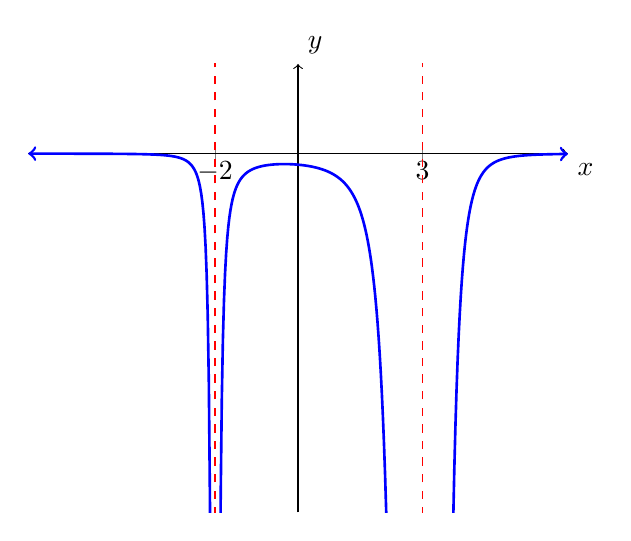
\begin{tikzpicture}
            \begin{axis}[
              axis lines=center,
              axis line style={->},
              xmin=-6.5, xmax=6.5,
              ymin=-4, ymax=1,
              xtick={-2,3},
              ymajorticks=false,
              ticklabel style={font=\normalsize,inner sep=0.5pt,fill=white,opacity=1.0, text opacity=1},
              xlabel=$x$, xlabel style={at={(ticklabel* cs:1)},anchor=north west},
              ylabel=$y$, ylabel style={at={(ticklabel* cs:1)},anchor=south west},
              every axis plot/.append style={line width=0.95pt}
              ]
              \addplot[<->] expression[domain=-6.5:6.5, restrict y to domain*=-7.5:1, blue, samples=500, unbounded coords=jump] {-40/((x+2)^2*(x-3)^4)};
              \draw[dashed,red] (-2,-7) -- (-2,5);
              \draw[dashed,red] (3,-7) -- (3,5);
            \end{axis}
          \end{tikzpicture}
        \end{minipage}%
        \begin{minipage}[t]{0.55\linewidth}\ 

          \begin{enumerate}
            \item $\ds\lim_{x \to -2^-} p(x)$
            \item $\ds\lim_{x \to -2^+} p(x)$
            \item $\ds\lim_{x \to -2}   p(x)$
            \item $\ds\lim_{x \to 3^-}  p(x)$
            \item $\ds\lim_{x \to 3^+}  p(x)$
            \item $\ds\lim_{x \to 3}    p(x)$
          \end{enumerate}
        \end{minipage}
      \end{ex*}
      \vspace*{\stretch{1}}
      \pagebreak
      
      \textit{Note:} When computing the limit, $\ds\lim_{x \to a} f(x)$ we can try to evaluate $f(a)$. 
      
      If $f(a)$ is of the form $\dfrac{0}{0}$, try factoring, conjugates, etc. (Section 2.3)\\
      
      If $f(a)$ is of the form $\dfrac{c}{0}$ where $c\neq 0$, the limit is infinite. Here, we must consider the signs of the numerator and the denominator.
      
      \begin{center}
        \begin{minipage}{0.4\linewidth}
          \begin{align*}
            \lim_{x \to 3^+} \frac{\overbrace{2-5x}^{-13}}{\underbrace{x-3}_{\text{small pos}}}=-\infty
          \end{align*}
        \end{minipage}%
        \begin{minipage}{0.4\linewidth}
          \begin{align*}
            \lim_{x \to 3^-} \frac{\overbrace{2-5x}^{-13}}{\underbrace{x-3}_{\text{small neg}}}=\infty
          \end{align*}
        \end{minipage}
      \end{center}
      
      \begin{ex*}
        Evaluate:
        \begin{tasks}(3)
          \task $\ds\lim_{x \to 3^-} \dfrac{2}{\parens{x-3}^3}$
          \task $\ds\lim_{x \to 3^+} \dfrac{2}{\parens{x-3}^3}$
          \task $\ds\lim_{x \to 3}   \dfrac{2}{\parens{x-3}^3}$
        \end{tasks}
        \vspace*{\stretch{1}}
      \end{ex*}
      
      \begin{ex*}
        For $h(t)=\dfrac{t^2-4t+3}{t^2-1}$, find $\ds\lim_{t \to 1} h(t)$ and $\ds\lim_{t \to -1} h(t)$.
        
        \vspace*{\stretch{1}}
        
        Are these infinite limits or limits at infinity?
      \end{ex*}
      \pagebreak
      
      \begin{ex*}
        Evaluate $\ds\lim_{\nu \to 7} \dfrac{4}{\parens{\nu-7}^2}$.
        \vspace*{\stretch{1}}
      \end{ex*}
      \begin{ex*}
        Evaluate $\ds\lim_{r \to 1} \dfrac{r}{\abs{r-1}}$.
        \vspace*{\stretch{1}}
      \end{ex*}
      \pagebreak
      
      \begin{ex*} Evaluate \end{ex*}
      \noindent
      \begin{minipage}{0.5\linewidth}
        \begin{itemize}
          \item $\ds\lim_{x \to \pi/2^-}  \tan x$
          \item $\ds\lim_{x \to \pi/2^+}  \tan x$
          \item $\ds\lim_{x \to -\pi/2^-} \tan x$
          \item $\ds\lim_{x \to -\pi/2^+} \tan x$
        \end{itemize}
      \end{minipage}
      \begin{minipage}{0.5\linewidth}
        \begin{flushright}
          \begin{tikzpicture}
            \begin{axis}[
              axis lines=center,
              axis line style={->},
              xmin=-1.25*pi, xmax=1.25*pi,
              ymin=-6, ymax=6,
              xtick={-3.14159265359, -1.570796326795, ..., 3.14159265359},
              xticklabels={$-\pi$, $-\frac{\pi}{2}$,, $\frac{\pi}{2}$, $\pi$},
              ymajorticks=false,
              ]
            \end{axis}
          \end{tikzpicture}
        \end{flushright}
      \end{minipage}

      \begin{ex*}
        Below is the graph of $\ln(x)$. Use this to evaluate the following limits:
      \end{ex*}  
      \noindent
      \begin{minipage}{0.3\linewidth}
        \begin{itemize}
          \item $\ds\lim_{x \to 0^+} \ln(x)$\\[15pt]
          \item $\ds\lim_{x \to \infty} \ln(x)$
        \end{itemize}
        \vspace*{50pt}
      \end{minipage}%
      \begin{minipage}{0.7\linewidth}
        \begin{flushright}
          \begin{tikzpicture}
            \begin{axis}[
              axis lines=center, 
              axis line style={->},
              xmin=-0.5, xmax=8.5,
              ymin=-4, ymax=4,
              ymajorticks=false,
              every axis plot/.append style={line width=0.95pt}
              ]
              \addplot[<->] expression[domain=0.018:8, samples=500, blue] {ln(x)};
            \end{axis}
          \end{tikzpicture}
        \end{flushright}
      \end{minipage}

      \begin{ex*}
        Find all vertical asymptotes, $x=a$, for $f(x)=\dfrac{\cos x}{x^2+2x}$.
      \end{ex*}
      \vspace*{\stretch{1}}
      \pagebreak
\end{document}

  \documentclass[answers]{exam}
\usepackage{texPreamble}
\usepackage{relsize}
\usepackage{tabularx}
\extraheadheight{0.25in}
\extrafootheight{1.0in}
\extrawidth{1in}
% ----------------------------------------------------------------
\makeatletter
\title{Fall 2018 Class notes}
\author{\thefname\ \thelname}

\pagestyle{headandfoot}

\firstpageheader{\@title\\\@date}{}{Math 1040}
\firstpageheadrule
%} %TODO 
\newcommand{\currentname}{\@currentlabelname}

\runningfootrule
\runningfooter{\currentname}{\thepage}{\@title}
\makeatother
\begin{document}
%\relscale{1.4}
\section{2.5: Limits at Infinity} 
      \begin{defn*}
        \textbf{Limits at Infinity and Horizontal Asymptotes} 

          If $f(x)$ becomes arbitrarily close to a finite number $L$ for all sufficiently large and positive $x$, then we write
            $$\lim_{x \to \infty} f(x)=L$$
          We say the limit of $f(x)$ as $x$ approaches infinity is $L$. In this case, the line $y=L$ is a \textbf{horizontal asymptote} of $f$. The limit at negative infinity, 
            $$\lim_{x \to -\infty} f(x)=M$$
          is defined analogously. When this limit exists, $y=M$ is a horizontal asymptote.
      \end{defn*}
      \begin{enumerate}[label=]
        \item\textit{Note:} The function \textit{can} cross it's horizontal asymptote (consider $\frac{\sin x}{x}$).
        \item\textit{Note:} A function can have 0, 1 or 2 horizontal asymptotes.
      \end{enumerate}
      
      \begin{ex*}
        For each of the following functions, find $\ds\lim_{x \to \infty} f(x)$ and $\ds\lim_{x \to -\infty} f(x)$.
      \end{ex*}
      \begin{tasks}(2)
        \task $f(x)=\dfrac{1}{x^2}$
        \task $f(x)=\dfrac{1}{x^3}$
      \end{tasks}
        \pagebreak
      \begin{tasks}[resume, after-item-skip=\stretch{1}](2)
        \task $f(x)=2+\dfrac{10}{x^2}$
        \task $f(x)=5+\dfrac{\sin x}{\sqrt x}$
        \task $f(x)=\parens{5+\dfrac{1}{x}+\dfrac{10}{x^2}}$
        \task $f(x)=\parens{3x^{12}-9x^7}$
        \task $f(x)=\sin(x)$
        \task $f(x)=\dfrac{\sin x}{x}$
      \end{tasks}
      \vspace*{\stretch{1}}
      \pagebreak
      %\def\currentname{2.5 Limits at Infinity} 
      \begin{defn*}
        \textbf{Infinite Limits at Infinity}
        If $f(x)$ becomes arbitrarily large as $x$ becomes arbitrarily large, then we write
          $$\lim_{x \to \infty} f(x)=\infty$$
        The limits $\ds\lim_{x \to \infty}=-\infty,\ds\lim_{x \to -\infty}=\infty$ and $\ds\lim_{x \to -\infty}=-\infty$ are defined similarly.
      \end{defn*}
      \begin{center}
        \begin{tikzpicture}[scale=0.9]
          \begin{groupplot}[
            group style={group size=2 by 2, horizontal sep=2cm, vertical sep=2.2cm},
            axis lines=center, 
            axis line style={->},
            xmin=-4.5, xmax=4.5,
            ymin=-5, ymax=40,
            ymajorticks=false,
            every axis plot/.append style={line width=0.95pt},
            ylabel=Even functions, ylabel style={at={(ticklabel* cs:1.1)},anchor=south},
            ]
          \nextgroupplot
            \addplot[<->] expression[domain=-4.5:4.5, blue, samples=50] {x^2};
            \addplot[<->] expression[domain=-2.52:2.52, red, samples=50] {x^4};
            \addplot[<->] expression[domain=-1.85:1.85, black, samples=50] {x^6};
          \nextgroupplot[
            ymin=-40, ymax=40,
            ylabel=Odd functions
            ]
            \addplot[<->] expression[domain=-3.4:3.4, blue, samples=50] {x^3};
            \addplot[<->] expression[domain=-2.09:2.09, red, samples=50] {x^5};
            \addplot[<->] expression[domain=-1.69:1.69, black, samples=50] {x^7};
          \nextgroupplot[
            ymin=-5, ymax=40,
            ylabel=$1/x^n:\ n$ Even
            ]
            \addplot[<->] expression[domain=-4.5:-0.158, blue, samples=50] {x^(-2)};
            \addplot[<->] expression[domain=0.158:4.5, blue, samples=50] {x^(-2)};
            \addplot[<->] expression[domain=-4.5:-0.3976, red, samples=50] {x^(-4)};
            \addplot[<->] expression[domain=0.3976:4.5, red, samples=50] {x^(-4)};
            \addplot[<->] expression[domain=-4.5:-0.541, black, samples=50] {x^(-6)};
            \addplot[<->] expression[domain=0.541:4.5, black, samples=50] {x^(-6)};
          \nextgroupplot[
            ymin=-40, ymax=40,
            ylabel=$1/x^n:\ n$ Odd
            ]
            \addplot[<->] expression[domain=-4.5:-0.2924, blue, samples=50] {x^(-3)};
            \addplot[<->] expression[domain=0.2924:4.5, blue, samples=50] {x^(-3)};
              \addlegendentry{$1/x^3$};
            \addplot[<->] expression[domain=-4.5:-0.4782, red, samples=50] {x^(-5)};
            \addplot[<->] expression[domain=0.4782:4.5, red, samples=50] {x^(-5)};
              \addlegendentry{$1/x^5$};
            \addplot[<->] expression[domain=-4.5:-0.5904, black, samples=50] {x^(-7)};
            \addplot[<->] expression[domain=0.5904:4.5, black, samples=50] {x^(-7)};
              \addlegendentry{$1/x^7$};
          \end{groupplot}
        \end{tikzpicture}
      \end{center}
      \pagebreak
       
      \begin{center}
        \fbox{\parbox{0.9\linewidth}{
        \begin{Thm*}
          \textbf{Limits at Infinity of Powers and Polynomials}
          
          Let $n$ be a positive integer and let $p$ be the polynomial 
            $$p(x)=a_nx^n+a_\nmo x^\nmo+\cdots+a_2x^2+a_1x+a_0, \text{ where } a_n\neq 0.$$
          \begin{enumerate}
            \item $\ds\lim_{x \to \pm \infty} x^n=\infty$ when $n$ is even.
            \item $\ds\lim_{x \to \infty} x^n=\infty$ and $\ds\lim_{x \to -\infty} x^n=-\infty$ when $n$ is odd.
            \item $\ds\lim_{x \to \pm\infty} \dfrac{1}{x^n}=\ds\lim_{x \to \pm\infty}x\inv[n]=0$.
            \item $\ds\lim_{x \to \pm\infty} p(x)=\lim_{x \to \pm\infty} a_nx^n=\pm\infty$, depending on the degree of the polynomial and the sign of the leading coefficient $a_n$.
          \end{enumerate}
        \end{Thm*}}}
      \end{center}
      \begin{enumerate}[label=]
        \item \textit{Note:} All previous limit laws still apply (e.g. constant multiplier rule)
        \item \textit{Note:} This theorem \textit{ONLY} applies for $x\to\pm\infty$. When $x\to a, \abs{a}<\infty$, we compute the left and right limits and use sm+/sm- (as done in section 2.4).
      \end{enumerate}
      \begin{ex*}
        For the following, find the limits as $x\to-\infty$ and $x\to \infty$:
        \begin{tasks}[after-item-skip=\stretch{1}](2)
          \task[] $f(x)=2x\inv[8]$
          \task[] $g(x)=-12x\inv[5]$
          \task[] $h(x)=3x^{12}-9x^7$
          \task[] $\ell(x)=2x\inv[8]+4x^3$
        \end{tasks}
        \vspace*{\stretch{1}}
      \end{ex*}
      \pagebreak 
      
      When finding the limit as $x\to\pm\infty$ of a rational function, $\frac{p(x)}{q(x)}$, where $p(x)$ and $q(x)$ are polynomial functions, we multiply the function by $\dfrac{\sfrac{1}{x^n}}{\sfrac{1}{x^n}}$, where $n$ is the highest degree in the denominator $q(x)$.
      
      \textit{Note:} To receive full credit for questions of this type, you must show all the fractions in your intermediate steps.
      \begin{ex*}\ 
      
        \begin{tasks}(1)
          \task $\ds\lim_{x \to \infty}\dfrac{1-x}{2x}$\\[50pt]
          \task $\ds\lim_{x \to \infty}\dfrac{1-x}{x^2}$\\[50pt]
          \task $\ds\lim_{x \to \infty}\dfrac{1-x^2}{2x}$
        \end{tasks}
      \end{ex*}
      \pagebreak
      
      \begin{center}
      \fbox{\parbox{0.95\linewidth}{
        \begin{Thm*}
          \textbf{End Behavior and Asymptotes of Rational Functions}
          
          Suppose $f(x)=\dfrac{p(x)}{q(x)}$ is a rational function, where 
            \begin{align*}
              p(x)&= a_mx^m+a_\mmo x^\mmo+\cdots+a_2x^2+a_1x+a_0\\
              q(x)&= b_nx^n+b_\nmo x^\nmo+\cdots+b_2x^2+b_1x+b_0
            \end{align*}
          with $a_m\neq0$ and $b_n\neq 0$.
          \begin{enumerate}
            \item \textbf{Degree of numerator less than degree of denominator}
            
            If $m<n$, then $\lim_{x \to \pm\infty} f(x)=0$ and $y=0$ is a horizontal asymptote of $f$.
            \item \textbf{Degree of numerator equals degree of denominator}
            
            If $m=n$, then $\lim_{x \to \pm\infty} f(x)=a_m/b_n$ and $y=a_m/b_n$ is a horizontal asymptote of $f$.
            \item \textbf{Degree of numerator greater than degree of denominator}
            
            If $m>n$, then $\lim_{x \to \pm\infty} f(x)=\infty$ or $-\infty$ and $f$ has no horizontal asymptote.
            \item \textbf{Slant Asymptote}
            
            If $m=n+1$, then $\lim_{x \to \pm \infty}f(x)=\infty$ or $-\infty$, and $f$ has no horizontal asymptote, but $f$ has a slant asymptote.
            \item \textbf{Vertical asymptotes}
            
            Assuming $f$ is in reduced form ($p$ and $q$ share no common factors), vertical asymptotes occur at the zeros of $q$.
          \end{enumerate}
        \end{Thm*}}}
      \end{center}
      \pagebreak
      
      \begin{ex*}
        Evaluate the limits of the following as $x\to-\infty$ and $x\to\infty$. State the equation of the horizontal asymptote.
        \begin{enumerate}
          \item $f(x)=\dfrac{2x^3+7}{x^3-x^2+x+7}$
            \vspace*{\stretch{1}}
          \item $g(x)=\dfrac{1}{x^3-4x+1}$
            \vspace*{\stretch{1}}
          \item $h(x)=\dfrac{3x^5+2x^2-2}{4x^4-3x}$
            \vspace*{\stretch{1}}
          \item $j(x)=\dfrac{4x^2-2x+3}{7x^2-1}$
            \vspace*{\stretch{1}}
          \item $\ell(x)=\dfrac{1-x^2}{3+2x-x^3}$
            \vspace*{\stretch{1}}
        \end{enumerate}
      \end{ex*}
      \pagebreak
      
      \begin{defn*}
      When the degree of the numerator, $m$, is greater than the degree of the denominator, $n$, the function has an oblique asymptote:
        $$f(x)=\dfrac{p(x)}{q(x)}=a(x)+\dfrac{r(x)}{q(x)}$$
      where $a(x)$ is the resulting polynomial that we get from polynomial long division and $r(x)$ is the remainder. We are interested in the special case where $m=n+1$, and $f(x)$ has a \textbf{slant asymptote}.
      \end{defn*}
      \begin{ex*}
        For the following functions, find the vertical asymptotes and the slant asymptotes:
      \end{ex*}
      \begin{enumerate}[itemsep=\stretch{1}]
        \item $y=\dfrac{2x^3+x^2+x+3}{x^2+2x}$
        \item $f(x)=\dfrac{x^2-1}{x+2}$
      \end{enumerate}
      \vspace*{\stretch{1}}
      \pagebreak
      \begin{enumerate}[itemsep=\stretch{1}]
        \setcounter{enumi}{2}
        \item $g(t)=\dfrac{t^2-1}{2t+4}$
        \item $h(u)=\dfrac{u^2}{u-1}$
      \end{enumerate}
      \vspace*{\stretch{1}}
      \pagebreak
      If the denominator has a square root, we need to change our work depending on if $x\to-\infty$ or $x\to\infty$:\\
      
      \begin{ex*}
        For the following, find the equation of the horizontal asymptotes:
        
      \noindent
      \begin{minipage}[t]{0.5\linewidth}
          \vspace*{20pt}
          \begin{tasks}[after-item-skip=0.10\paperheight](1)
            \task $\ds\lim_{x \to \infty}\dfrac{x}{\sqrt{x^2+3}}$
            \task $\ds\lim_{x \to-\infty}\dfrac{x}{\sqrt{x^2+3}}$
            \task $\ds\lim_{x \to \infty}\dfrac{x}{\sqrt{x^2+x}}$
            \task $\ds\lim_{x \to-\infty}\dfrac{x}{\sqrt{x^2+x}}$
          \end{tasks}
      \end{minipage}%
      \begin{minipage}[t]{0.5\linewidth}\ 
      
        \begin{flushright}
          \begin{tikzpicture}
            \begin{axis}[
              axis lines=center,
              axis line style={->},
              xmin=-6.5, xmax=6.5,
              ymin=-2.25, ymax=2.25,
              ticklabel style={font=\tiny,inner sep=0.75pt,fill=white},
              xlabel=$x$, xlabel style={at={(ticklabel* cs:1)},anchor=north west},
              ylabel=$y$, ylabel style={at={(ticklabel* cs:1)},anchor=south west},
              every axis plot/.append style={line width=0.95pt},
              legend style={at={(axis cs:1.25,-1.5)},draw=none,anchor=south west},
              ]
              \addplot[<->] expression[domain=-6:6, blue] {x/(sqrt(x^2+3)};
                \addlegendentry{$\frac{x}{\sqrt{x^2+3}}$};
            \end{axis}
          \end{tikzpicture}
        \end{flushright}
      \end{minipage}%
      \end{ex*}
      \vspace*{\stretch{1}}
      \pagebreak
      \begin{tasks}[resume, after-item-skip=0.2\paperheight](1)
        \task $\dfrac{7x^3-2}{-x^3+\sqrt{25x^6+4}}$
        \task $\dfrac{\sqrt[3]{x^6+8}}{4x^2+\sqrt{3x^4+1}}$
        \task $\dfrac{2x}{\sqrt{x^2-x-2}}$
      \end{tasks}
      \pagebreak
      
      \begin{ex*}
        For the following, sketch a graph with the following properties:
        
        \noindent
        \begin{minipage}[t]{0.35\linewidth}\ 
        
          \begin{enumerate}
            \item 
              \begin{enumerate}[label=]
                \itemsep10pt 
                \item $\ds\lim_{x \to 0} f(x)=-\infty$
                \item $\ds\lim_{x \to 2} f(x)=\dfrac{5}{4}$
                \item $\ds\lim_{x \to \pm\infty} f(x)=1$
                \item $f(2)$ DNE
                \item $f(1)=1$
                \item $f(-1)=-1$
              \end{enumerate}
          \end{enumerate}
          
        \end{minipage}%
        \begin{minipage}[t]{0.65\linewidth}\ 
          \begin{flushright}
            \begin{tikzpicture}[scale=1.3]
              \begin{axis}[
                grid=both,
                grid style={line width=0.35pt, draw=gray!75},
                axis lines=center,
                axis line style={->},
                xmin=-5, xmax=5,
                ymin=-5, ymax=5,
                xtick={-5,-4,...,5},
                ytick={-5,-4,...,6},
                enlargelimits={abs=0.75},
                ticklabel style={font=\tiny,inner sep=0.75pt,fill=white},
                xlabel=$x$, xlabel style={at={(ticklabel* cs:1)},anchor=north west},
                ylabel=$y$, ylabel style={at={(ticklabel* cs:1)},anchor=south west},
                every axis plot/.append style={line width=0.95pt}
                ]
              \end{axis}
            \end{tikzpicture}
          \end{flushright}
        \end{minipage}
        
        \vspace*{\stretch{1}}
        \noindent
        \begin{minipage}[t]{0.35\linewidth}\ 
        
          \begin{enumerate}
            \setcounter{enumi}{1}
            \item 
              \begin{enumerate}[label=]
                \itemsep10pt 
                \item $\ds\lim_{x \to -1^-} f(x)=\infty$
                \item $\ds\lim_{x \to -1^+} f(x)=-\infty$
                \item $\ds\lim_{x \to \pm\infty} f(x)=2$
                \item $f(0)=-2$
                \item $f(1)=1$
                \item $f(-2)=4$
              \end{enumerate}
          \end{enumerate}
          
        \end{minipage}%
        \begin{minipage}[t]{0.65\linewidth}\ 
        
          \begin{flushright}
            \begin{tikzpicture}[scale=1.3]
              \begin{axis}[
                grid=both,
                grid style={line width=0.35pt, draw=gray!75},
                axis lines=center,
                axis line style={->},
                xmin=-5, xmax=5,
                ymin=-5, ymax=5,
                xtick={-5,-4,...,5},
                ytick={-5,-4,...,6},
                enlargelimits={abs=0.75},
                ticklabel style={font=\tiny,inner sep=0.75pt,fill=white},
                xlabel=$x$, xlabel style={at={(ticklabel* cs:1)},anchor=north west},
                ylabel=$y$, ylabel style={at={(ticklabel* cs:1)},anchor=south west},
                every axis plot/.append style={line width=0.95pt}
                ]
              \end{axis}
            \end{tikzpicture}
          \end{flushright}
        \end{minipage}
      \end{ex*}
      \pagebreak
      
      \begin{ex*}
        Find \textit{all} asymptotes (vertical, horizontal, slant)
        \begin{enumerate}
          \item $\dfrac{x^3-10x^2+16x}{x^2-8x}$
            \vspace*{\stretch{1}}
          \item $\dfrac{\cos x+2\sqrt x}{\sqrt x}$
            \vspace*{\stretch{1}}
        \end{enumerate}
      \end{ex*}
      \def\currentname{2.5 Limits at Infinity}
      \pagebreak
      \def\currentname{2.5 Limits at Infinity}
      
      Other function end behavior to consider include $e^x, e\inv[x], \ln(x)$ and $\tan\inv(x)$:
      \begin{center}
        \begin{tikzpicture}
          \begin{groupplot}[
            group style={group size=2 by 2, horizontal sep=2cm, vertical sep=2cm},
            axis lines=center,
            axis line style={->},
            xmin=-6.5, xmax=6.5,
            ymin=-2.25, ymax=6.5,
            ticklabel style={font=\tiny,inner sep=0.75pt,fill=white},
            xlabel=$x$, xlabel style={at={(ticklabel* cs:1)},anchor=north west},
            ylabel=$y$, ylabel style={at={(ticklabel* cs:1)},anchor=south west},
            every axis plot/.append style={line width=0.95pt},
            legend style={at={(axis cs:6,-2)},anchor=south east},
            ]
          \nextgroupplot
            \addplot[<->] expression[domain=-6:1.8, blue, samples=100] {e^x};
              \addlegendentry{$e^x$};
          \nextgroupplot
            \addplot[<->] expression[domain=-1.8:6, blue, samples=100] {e^(-x)};
              \addlegendentry{$e\inv[x]$};
          \nextgroupplot[
            xmin=-0.5, xmax=8.5,
            ymin=-4.5, ymax=4.5,
            legend style={at={(axis cs:8,-4)},anchor=south east},
            ]
            \addplot[<->] expression[domain=0.0111:8, samples=500, blue] {ln(x)};
              \addlegendentry{$\ln(x)$};
          \nextgroupplot[
            xmin=-6.5, xmax=6.5,
            ymin=-2.25, ymax=2.25,
            legend style={at={(axis cs:6,-2)},anchor=south east},
            ]
            \addplot[<->] expression[domain=-6.45:6.45, samples=500, blue] {rad(atan(x))};
              \addlegendentry{$\tan\inv(x)$};
          \end{groupplot}
        \end{tikzpicture}
      \end{center}
      \def\currentname{2.5 Limits at Infinity}
      \vspace*{\stretch{0.2}}
      \begin{tasks}[after-item-skip=\stretch{1}](2)
        \task $\ds\lim_{x \to -\infty}\sin x$
        \task $\ds\lim_{x \to \infty}\sin x$
        \task $\ds\lim_{x \to -\infty}\cos x$
        \task $\ds\lim_{x \to \infty}\cos x$
      \end{tasks}
      \vspace*{\stretch{1}}
      \pagebreak
      \def\currentname{2.5 Limits at Infinity}
\end{document}

  \documentclass[mathNotesPreamble]{subfiles}
\begin{document}
%\relscale{1.4}
\section{JIT 6.1: The Family of Exponential Functions}
  \begin{defn*}
    An \textbf{exponential function} has the form $f(x)=a^x$, where $a>0$. The number $a$ is called the \textbf{base}.
  \end{defn*}
  \begin{ex*}\ 
  
    \noindent
    \begin{minipage}{0.5\linewidth}
      \begin{center}
        \begin{tabular}{@{}R@{\hspace*{35pt}}L@{\ =\,}L@{}}\toprule
          x& \multicolumn{2}{C}{f(x)}\\\midrule
          -1& 2\inv&\sfrac12\\
          0& 2^0&1\\
          \sfrac12& 2^{\sfrac{1}{2}}&\sqrt2\\
          2& 2^2&4\\
          3.2& 2^3\cdot2^{\sfrac{1}{5}}&8\sqrt[5]{2}\\\bottomrule
        \end{tabular}
      \end{center}
    \end{minipage}%
    \begin{minipage}{0.5\linewidth}
      \begin{center}
        \begin{tikzpicture}
          \begin{axis}[
            grid=both,
            grid style={line width=0.35pt, draw=gray!75},
            axis lines=center,
            axis line style={->},
            xmin=-4, xmax=4,
            ymin=-2, ymax=6,
            xtick={-4,-3,...,4},
            ytick={-2,-1,...,6},
            enlargelimits={abs=0.75},
            ticklabel style={font=\tiny, inner sep=0.75pt,fill=white},
            xlabel=$x$, xlabel style={at={(ticklabel* cs:1)},anchor=north west},
            ylabel=$y$, ylabel style={at={(ticklabel* cs:1)},anchor=south west},
            every axis plot/.append style={line width=0.95pt}
            ]
            \addplot[<->] expression[domain=-4.75:2.75, blue] {2^x} node[inner sep=0.75pt, right, black, fill=white, pos=0.9, xshift=5pt] {$2^x$};
          \end{axis}
        \end{tikzpicture}
      \end{center}
    \end{minipage}%
  \end{ex*}
  \vfill
  The base $a$ determines if $a^x$ increases with exponential growth or decreases with exponential decay:
  
  \noindent
  \begin{minipage}{0.5\linewidth}
    \begin{center}
      $$a>1$$
      
        \begin{tikzpicture}
          \begin{axis}[
            grid=both,
            grid style={line width=0.35pt, draw=gray!75},
            axis lines=center,
            axis line style={->},
            xmin=-4, xmax=4,
            ymin=-2, ymax=6,
            xtick={-4,-3,...,4},
            ytick={-2,-1,...,6},
            enlargelimits={abs=0.75},
            ticklabel style={font=\tiny, inner sep=0.75pt,fill=white},
            xlabel=$x$, xlabel style={at={(ticklabel* cs:1)},anchor=north west},
            ylabel=$y$, ylabel style={at={(ticklabel* cs:1)},anchor=south west},
            every axis plot/.append style={line width=0.95pt}
            ]
            \addplot[<->] expression[domain=-4.75:2.75, blue] {2^x} node[inner sep=0.75pt,right, black, fill=white, pos=0.9, xshift=5pt] {$2^x$};
          \end{axis}
        \end{tikzpicture}
      \end{center}
  \end{minipage}%
  \begin{minipage}{0.5\linewidth}
    \begin{center}
      $$0<a<1$$
      
        \begin{tikzpicture}
          \begin{axis}[
            grid=both,
            grid style={line width=0.35pt, draw=gray!75},
            axis lines=center,
            axis line style={->},
            xmin=-4, xmax=4,
            ymin=-2, ymax=6,
            xtick={-4,-3,...,4},
            ytick={-2,-1,...,6},
            enlargelimits={abs=0.75},
            ticklabel style={font=\tiny, inner sep=0.75pt,fill=white},
            xlabel=$x$, xlabel style={at={(ticklabel* cs:1)},anchor=north west},
            ylabel=$y$, ylabel style={at={(ticklabel* cs:1)},anchor=south west},
            every axis plot/.append style={line width=0.95pt}
            ]
            \addplot[<->] expression[domain=-2.75:4.75, blue] {0.5^x} node[inner sep=0.75pt,left, black, fill=white, pos=0.1, xshift=-5pt] {$\sfrac{1}{2}^x$};
          \end{axis}
        \end{tikzpicture}
      \end{center}
  \end{minipage}%
  \pagebreak
  
  \begin{ex*}
    Graph $3^x$ and $5^x$ on the axes provided below:
    \begin{center}
      \begin{tikzpicture}[scale=1.4]
        \begin{axis}[
          grid=both,
          grid style={line width=0.35pt, draw=gray!75},
          axis lines=center,
          axis line style={->},
          xmin=-4, xmax=4,
          ymin=-2, ymax=6,
          xtick={-4,-3,...,4},
          ytick={-2,-1,...,6},
          enlargelimits={abs=0.75},
          ticklabel style={font=\tiny, inner sep=0.75pt,fill=white},
          every axis plot/.append style={line width=0.95pt}
          ]
        \end{axis}
      \end{tikzpicture}
    \end{center}
  \end{ex*}
  
  \vspace*{\stretch{1}}
  \begin{ex*}
    Graph $\parens{\dfrac{1}{3}}^x$ and $\parens{\dfrac{1}{5}}^x$ on the axes provided below:
    \begin{center}
      \begin{tikzpicture}[scale=1.4]
        \begin{axis}[
          grid=both,
          grid style={line width=0.35pt, draw=gray!75},
          axis lines=center,
          axis line style={->},
          xmin=-4, xmax=4,
          ymin=-2, ymax=6,
          xtick={-4,-3,...,4},
          ytick={-2,-1,...,6},
          enlargelimits={abs=0.75},
          ticklabel style={font=\tiny, inner sep=0.75pt,fill=white},
          every axis plot/.append style={line width=0.95pt}
          ]
        \end{axis}
      \end{tikzpicture}
    \end{center}
  \end{ex*}
  
  \pagebreak
  \begin{ex*}
    Graph $\parens{\dfrac{6}{7}}^x$ and $\parens{\dfrac{7}{6}}^x$:
    \begin{center}
      \begin{tikzpicture}[scale=1.4]
        \begin{axis}[
          grid=both,
          grid style={line width=0.35pt, draw=gray!75},
          axis lines=center,
          axis line style={->},
          xmin=-4, xmax=4,
          ymin=-2, ymax=6,
          xtick={-4,-3,...,4},
          ytick={-2,-1,...,6},
          enlargelimits={abs=0.75},
          ticklabel style={font=\tiny, inner sep=0.75pt,fill=white},
          every axis plot/.append style={line width=0.95pt}
          ]
        \end{axis}
      \end{tikzpicture}
    \end{center}
  \end{ex*}
  \vspace*{\stretch{1}}
  
\section{JIT 6.2: The Function $e^x$}
  \currentname
  
  The number $e$ is an irrational number whose exact form is
    $$e=\lim_{n \to \infty}\parens{1+\dfrac{1}{n}}^n\approx2.718281828459045\dots$$
    $$e^x=1+x+\frac{x^2}{2!}+\frac{x^3}{3!}+\frac{x^4}{4!}+\dots=\sum\nto[0]^\infty \dfrac{x^n}{n!}$$
  This exponential function has a $45^\circ$ tangent at $x=0$. This function shows in many applications, and each function $a^x$ can be written as $e^{kx}$.
  
  \pagebreak
  
  \begin{ex*}
    Graph $2^x, e^x$ and $3^x$:
  \end{ex*}
  \begin{center}
    \begin{tikzpicture}[scale=1.375]
      \begin{axis}[
        grid=both,
        grid style={line width=0.35pt, draw=gray!75},
        axis lines=center,
        axis line style={->},
        xmin=-4, xmax=4,
        ymin=-2, ymax=6,
        xtick={-4,-3,...,4},
        ytick={-2,-1,...,6},
        enlargelimits={abs=0.75},
        ticklabel style={font=\tiny, inner sep=0.75pt,fill=white},
        every axis plot/.append style={line width=0.95pt}
        ]
      \end{axis}
    \end{tikzpicture}
  \end{center}
  \vspace*{\stretch{1}}

  \noindent
  All exponential functions follow the all the typical rules when performing transformation of functions:
  \begin{ex*}
    Graph $y=3^x,\ y=3^{x-1},\ y=3^{x+3},\ y=3^x+2,\ y=-3^x,\ y=3\inv[x]$
  \end{ex*}
  \begin{center}
    \begin{tikzpicture}[scale=1.375]
      \begin{axis}[
        grid=both,
        grid style={line width=0.35pt, draw=gray!75},
        axis lines=center,
        axis line style={->},
        xmin=-4, xmax=4,
        ymin=-2, ymax=6,
        xtick={-4,-3,...,4},
        ytick={-2,-1,...,6},
        enlargelimits={abs=0.75},
        ticklabel style={font=\tiny, inner sep=0.75pt,fill=white},
        every axis plot/.append style={line width=0.95pt}
        ]
      \end{axis}
    \end{tikzpicture}
  \end{center}

  
  \pagebreak
  \begin{ex*}\ 
  
  \noindent
  \begin{minipage}[t]{0.625\linewidth}
    
    Solve:
    \begin{tasks}[after-item-skip=0.125\paperheight](1)
      \task $2^{x-3}=64$
      \task $4^{2x-3}=64$
    \end{tasks}
  \end{minipage}%
  \begin{minipage}[t]{0.375\linewidth}\ 
  
    \flushright
    \fbox{\parbox{0.85\linewidth}{
    \underline{Properties of exponents}
    \begin{enumerate}
      \item $a^m\cdot a^n=a^{m+n}$
      \item $\dfrac{a^m}{a^n}=a^{m-n}$
      \item $\parens{a^m}^n=a^{mn}$
      \item $\parens{ab}^n=a^nb^n$
      \item $\parens{\dfrac{a}{b}}^n=\dfrac{a^n}{b^n}, b\neq 0$
      \item $a\inv[n]=\frac{1}{a^n}, a\neq 0$
      \item $a^0=1, a\neq 0$
    \end{enumerate}
  }}
  \end{minipage}%
  \begin{tasks}[resume, after-item-skip=0.075\paperheight](3)
    \task $10^{\sin x}=1$
    \task $5^{x^2+2x}=125$
    \task $\parens{\dfrac{1}{4}}^{2-x}=16^x$
  \end{tasks}
  \end{ex*}
  \vspace*{\stretch{1}}
  
  \begin{ex*}
    Simplify:
    \begin{tasks}(3)
      \task $\parens{e^x}^3$
      \task $\dfrac{e^{2x}}{e^x}$
      \task $\dfrac{e^{2x}-1}{e^x-1}$
    \end{tasks}
  \end{ex*}
  \vspace*{\stretch{1}}
  
  \pagebreak
  
  \section{JIT 7.1: Composition and Inverse Functions}
  
  \begin{defn*}
    Given two functions $f$ and $g$, the composite function $f\circ g$ is defined by $(f\circ g)(x)=f\parens{g(x)}$. It is evaluated in two steps: $y=f(u)$, where $u=g(x)$. The domain of $f\circ g$ consists of all $x$ in the domain of $g$ such that $u=g(x)$ is in the domain of $f$.
  \end{defn*}
  \begin{ex*}
    Given $f(x)=x^2+2x+\pi$ and $g(x)=x^2$, find
    \begin{itemize}[label=, itemsep=\stretch{1}]
      \item $f\parens{g(x)}$
      \item $g\parens{f(x)}$
    \end{itemize}
  \end{ex*}
  \vspace*{\stretch{1}}
  \begin{ex*}
    Given $f(x)=\dfrac{1}{x+2}$ and $g(x)=x^2-1$, find
    \begin{itemize}[label=, itemsep=\stretch{1}]
      \item $f\parens{g(x)}$
      \item $g\parens{f(x)}$
    \end{itemize}
  \end{ex*}
  \vspace*{\stretch{1}}
  \begin{ex*}
    Given $f(x)=x^2, g(x)=\sin(x)$ and $h(x)=2x+1$, find 
    \begin{itemize}[label=, itemsep=\stretch{1}]
      \item $f(g(h(x)))$
    \end{itemize}
  \end{ex*}
  \vspace*{\stretch{1}}
  
  \pagebreak
  
  \begin{ex*}
    Given $f(x)=x^3, g(x)=\cos(x)$, find
    \begin{tasks}[after-item-skip=\stretch{1}](4)
      \task[] $f(0)$ 
      \task[] $f(1)$
      \task[] $g(0)$ 
      \task[] $(f\circ g)(0)$
      \task[] $(f\circ g)(x)$
      \task[] $(g\circ f)(x)$
      \task[] $(f\circ f)(x)$
      \task[] $(g\circ g)(x)$
    \end{tasks}
  \end{ex*}
  
  \vspace*{\stretch{1}}
  \begin{ex*}
    Evaluate or explain why the functions value is undefined:
  \end{ex*}
  \noindent
  \begin{minipage}[t]{0.5\linewidth}\ 
    
    \begin{enumerate}[label=,itemsep=15pt]
      \item $f\parens{g(2)}$
      \item $g\parens{f(2)}$
      \item $\parens{f\circ g}(0)$
      \item $\parens{g\circ f}(6)$
      \item $\parens{g\circ g}(-2)$
      \item $\parens{f\circ f}(4)$
    \end{enumerate}
    \vspace*{15pt}
  \end{minipage}%
  \begin{minipage}[t]{0.5\linewidth}\ 
  
    \begin{flushright}
      \begin{tikzpicture}
        \begin{axis}[
          grid=both,
          grid style={line width=0.35pt, draw=gray!75},
          axis lines=center,
          axis line style={->},
          xmin=-4, xmax=6,
          ymin=-2, ymax=6,
          xtick={-4,-3,...,6},
          ytick={-2,-1,...,6},
          enlargelimits={abs=0.75},
          ticklabel style={font=\tiny, inner sep=0.75pt,fill=white},
          every axis plot/.append style={line width=0.95pt}
          ]
          \addplot[-] expression[domain=-4:0, blue] {(0.5*(x+2))^2+2};
          \addplot[-] expression[domain=0:2, blue] {x+3};
          \addplot[-] expression[domain=2:4, blue] {sqrt(4-(x-2)^2)+3} node[inner sep=0.75pt, above, black, pos=0.15, fill=white, yshift=3pt] {$g(x)$};
          %
          \addplot[-] expression[domain=0:2, red] {-x};
          \addplot[-] expression[domain=2:6, red] {2*x-6} node[inner sep=0.75pt, right, black, pos=0.6, fill=white, xshift=4pt] {$f(x)$};
        \end{axis}
      \end{tikzpicture}
    \end{flushright}
  \end{minipage}
  \begin{description}
    \item[Note:] $f\parens{g(x)}$ is not necessarily the same as $g\parens{f(x)}$.
    \item[Note:] If $f\parens{g(x)}=x$ and $g\parens{f(x)}=x$, then $f(x)$ and $g(x)$ are inverse functions.
  \end{description}
  \pagebreak
  
\end{document}

  \documentclass[answers]{exam}
\usepackage{texPreamble}
\usepackage{relsize}
\usepackage{tabularx}
\usepackage{scrextend}
\extraheadheight{0.25in}
\extrafootheight{1.0in}
\extrawidth{1in}
% ----------------------------------------------------------------

\begin{document}
%\relscale{1.4}
\section{JIT 7.2: The Ideas of Inverses}
  \begin{defn*}[Inverse function]
    Given a function $f$, its inverse (if it exists) is a function $f\inv$ such that whenever $y=f(x)$, then $f\inv(y)=x$.
  \end{defn*}
  \vfill
  %\begin{addmargin}[30pt]{0pt}
    \begin{description}
      \item[Note:] $f$ and $g$ are inverses if $f\parens{g(x)}=x$ \textit{and} $g\parens{f(x)}=x$.
      \item[Note:] The domain of $f(x)$ must be the range of $g(x)$.
      \item[Note:] The domain of $g(x)$ must be the range of $f(x)$.
      \item[Note:] The inverse, $f\inv(x)$, should \textbf{not} be confused with $\sbrkt{f(x)}\inv=\dfrac{1}{f(x)}$.
    \end{description}
  %\end{addmargin}
  \pagebreak
  \begin{ex*}
    For the following, verify that $f(x)$ and $g(x)$ are inverses:
    \begin{enumerate}[label=,itemsep=25pt]
      \item $f(x)=x^2,\ x>0\\ g(x)=\sqrt x$
      \item $f(x)=\sfrac{1}{x}\\ g(x)=\sfrac{1}{x}$
      \item $f(x)=3x+2\\ g(x)=\dfrac{1}{3}(x-2)$
    \end{enumerate}
  \end{ex*}
  \vfill
  \begin{defn*}[One-to-One Functions and the Horizontal Line Test]
    A function $f$ is \textbf{one-to-one} on a domain $D$ if each value of $f(x)$ corresponds to exactly one value of $x$ in $D$. More precisely, $f$ is one-to-one on $D$ if $f(x_1)\neq f(x_2)$ whenever $x_1\neq x_2$, for $x_1$ and $x_2$ in $D$. 
    
    The \textbf{horizontal line test} says that every horizontal line intercepts the graph of a one-to-one function at most once.
  \end{defn*}
  \vfill
  \begin{center}
    \begin{tikzpicture}
      \begin{groupplot}[
        group style={group size=2 by 1, horizontal sep=2cm},
        axis lines=center,
        axis line style={->},
        xmin=-0.5, xmax=4,
        ymin=-0.125, ymax=2.5,
        xmajorticks=false,
        ymajorticks=false,
        enlargelimits={abs=0.75},
        ticklabel style={font=\tiny, inner sep=0.75pt,fill=white},
        every axis plot/.append style={line width=0.95pt}
        ]
      \nextgroupplot
        \addplot[->] expression[domain=0:4.5, blue, samples=50] {sqrt(x)};
      \nextgroupplot[
        xmin=-4.5, xmax=4.5,
        ymin=-64, ymax=64,
        ]
        \addplot[<->] expression[domain=-4:4, blue, samples=50] {x^3};
      \end{groupplot}
    \end{tikzpicture}
  \end{center}
  \vfill
  \pagebreak
  \noindent
  \begin{center}
    \begin{tikzpicture}
      \begin{groupplot}[
        group style={group size=2 by 1, horizontal sep=2cm},
        axis lines=center,
        axis line style={->},
        xmin=-6.5, xmax=6.5,
        xmajorticks=false,
        ymajorticks=false,
        enlargelimits={abs=0.75},
        ticklabel style={font=\tiny, inner sep=0.75pt,fill=white},
        every axis plot/.append style={line width=0.95pt}
        ]
      \nextgroupplot
        \addplot[<->] expression[domain=-2.3*pi:2.3*pi, blue, samples=100] {sin(\x r)};
      \nextgroupplot[
        xmin=-4, xmax=4,
        ymin=-2, ymax=16,
        ]
        \addplot[<->] expression[domain=-4:4, blue, samples=50] {x^2};
      \end{groupplot}
    \end{tikzpicture}
  \end{center}
  \vfill
  \begin{center}
    \fbox{\parbox{0.9\linewidth}{ \textbf{Existence of Inverse Functions}
    
    Let $f$ be a one-to-one function on a domain $D$ with a range $R$. Then $f$ has a unique inverse $f\inv$ with domain $R$ and range $D$ such that
      $$f\inv\parens{f(x)}=x\hspace*{50pt}\text{ and }\hspace*{50pt}f\parens{f\inv(y)}=y$$
    where $x$ is in $D$ and $y$ is in $R$.
    }}
  \end{center}
  \vfill
  \begin{ex*}
    Using the table below, solve the following:
    \vspace*{10pt}    
    
    \noindent
    \begin{minipage}{0.5\linewidth}
      \begin{enumerate}[label=,itemsep=12.5pt]
        \item $\parens{f\circ f}(-1)$
        \item $f\inv(2)$
        \item $f\inv(6)$
        \item $f\parens{f\inv(6)}$
        \item $f\inv\parens{f\inv(6)}$
      \end{enumerate}
    \end{minipage}%
    \begin{minipage}{0.5\linewidth}
      \begin{flushright}
        \begin{tabular}{@{}R@{\hspace*{15pt}}R@{}}\toprule
          x& f(x)\\\midrule
          -2&-8\\
          -1&-2\\
          0&0\\
          1&2\\
          2&6\\\bottomrule
        \end{tabular}
      \end{flushright}
    \end{minipage}%
  \end{ex*}
  \pagebreak
\section{JIT 7.3: Finding the Inverse of $f$ Given a Graph}
  \textit{Note:} A function is symmetric with it's inverse with respect to $y=x$.
  \vfill
  
  \begin{center}
    \begin{tabularx}{\linewidth}{*{3}{>{\centering\arraybackslash}X}}
      \begin{tabular}{@{}R@{\ =\ }L@{}}
        f(x)&\sqrt x\\
        f\inv(x)& x^2,\ x>0
      \end{tabular}&
      \begin{tabular}{@{}R@{\ =\ }L@{}}
        f(x)&x^3\\
        f\inv(x)& \sqrt[3]{x}=x^{\sfrac{1}{3}}
      \end{tabular}&  
      \begin{tabular}{@{}R@{\ =\ }L@{}}
        f(x)&\sin x \text{ on } \sbrkt{-\sfrac{\pi}{2},\sfrac{\pi}{2}}\\
        f\inv(x)& \sin\inv x
      \end{tabular}\\
    \end{tabularx}
    \begin{tikzpicture}[scale=0.75]
      \begin{groupplot}[
        group style={group size=3 by 1, horizontal sep=1.5cm},
        axis lines=center,
        axis line style={->},
        axis equal,
        xmin=-1, xmax=3,
        ymin=-1, ymax=3,
        xtick={-4,-3,...,4},
        ytick={-2,-1,...,6},
        enlargelimits={abs=0.75},
        ticklabel style={font=\tiny, inner sep=0.75pt,fill=white},
        xlabel=$x$, xlabel style={at={(ticklabel* cs:1)},anchor=north west},
        ylabel=$y$, ylabel style={at={(ticklabel* cs:1)},anchor=south west},
        every axis plot/.append style={line width=0.95pt}
        ]
      \nextgroupplot
        \addplot[->] expression[domain=0:4, blue, samples=50] {sqrt(x)};
        \addplot[->] expression[domain=0:1.9, red, samples=50] {x^2};
        \addplot[dashed] expression[domain=-2.5:4.5, black!50] {x};
      \nextgroupplot[
        xmin=-3, xmax=3,
        ymin=-3, ymax=3,
        ytick={-6,-5,...,6},
        ]
        \addplot[<->] expression[domain=-1.55:1.55, blue, samples=50] {x^3};
        \addplot[<->] expression[domain=-4.25:4.25, red, samples=100] {x/abs(x)*abs(x)^(1/3)};
        \addplot[dashed] expression[domain=-2.5:4.5, black!50] {x};
      \nextgroupplot[
        xmin=-0.45*pi, xmax=0.45*pi,
        ymin=-0.45*pi, ymax=0.45*pi,
        ]
        \addplot[<->] expression[domain=-0.5*pi:0.5*pi, blue, samples=50] {sin(\x r)};
        \addplot[<->] expression[domain=-1:1, red, samples=100] {rad(asin(x))};
        \addplot[dashed] expression[domain=-3:3, black!50] {x};
      \end{groupplot}
    \end{tikzpicture}
  \end{center}
  \vspace*{\stretch{1}}
  \begin{ex*}
    Draw the function's inverse:
    
    \noindent
    \begin{minipage}{0.5\linewidth}
      \begin{center}
        $$f(x)=2^x$$
        \begin{tikzpicture}[scale=1.25]
          \begin{axis}[
            axis lines=center,
            axis line style={->},
            xmin=-5, xmax=5,
            ymin=-5, ymax=5,
            xmajorticks=false,
            ymajorticks=false
            ]
          \end{axis}
        \end{tikzpicture}
      \end{center}
    \end{minipage}%
    \begin{minipage}{0.5\linewidth}
      \begin{center}
        $$f(x)=\sqrt{x+1}-2$$
        \begin{tikzpicture}[scale=1.25]
          \begin{axis}[
            axis lines=center,
            axis line style={->},
            xmin=-5, xmax=5,
            ymin=-5, ymax=5,
            xmajorticks=false,
            ymajorticks=false
            ]
          \end{axis}
        \end{tikzpicture}
      \end{center}
    \end{minipage}%
  \end{ex*}
  \pagebreak
\section{JIT 7.4: Finding the Inverse of $f$ Given by an Expression}
  {\centering\fbox{\parbox{0.95\linewidth}{
    \textbf{Finding an Inverse Function}
    
    Suppose $f$ is one-to-one on an interval $I$. To find $f\inv$, use the following steps:
    \begin{enumerate}
      \item Solve $y=f(x)$ for $x$. If necessary, choose the function that corresponds to $I$.
      \item Interchange $x$ and $y$ and write $y=f\inv(x)$.
    \end{enumerate}
  }}}
  \begin{ex*}
    Find $f\inv(x)$:
    \begin{enumerate}[label=, itemsep=50pt]
      \item $f(x)=x^2-2x+1,\ x\geq 1$
      \item $g(x)=\dfrac{x}{2}-\dfrac{7}{2}$
      \item $h(x)=\sqrt[3]{5x+1}$
      \item $j(x)=\dfrac{2x}{1-x}$
      \item $k(x)=e^x$
    \end{enumerate}
  \end{ex*}
  \pagebreak
  
  \begin{ex*}
    Find the inverse of $f(x)=\parens{x-1}^4$ (on a restricted domain) and graph $f(x)$ and $f\inv(x)$.
    \begin{flushright}
      \begin{tikzpicture}
        \begin{axis}[
          axis lines=center,
          axis line style={->},
          xmin=-4, xmax=4,
          ymin=-4, ymax=4,
          xmajorticks=false,
          ymajorticks=false,
          ]
        \end{axis}
      \end{tikzpicture}
    \end{flushright}
  \end{ex*}
  \vspace*{\stretch{1}}
  \pagebreak
\end{document}

  \documentclass[mathNotesPreamble]{subfiles}
\begin{document}
%\relscale{1.4}
\section{JIT 8.1: Definitions of Logarithms}
  \begin{defn*}[Logarithmic Function Base $b$]
    For any base $b>0$, with $b\neq 1$, the \textbf{logarithmic function base $b$}, denoted $y~=~\log_b(x)$, is the inverse of the exponential function $y=b^x$. The inverse of the natural exponential function with base $b=e$ is the \textbf{natural logarithm function}, denoted $y=\ln(x)$.
  \end{defn*}
  
  \noindent
  \begin{minipage}{0.5\linewidth}
    \begin{center}
      \begin{tikzpicture}
        \begin{axis}[
          axis lines=center,
          axis line style={->},
          axis equal,
          xmin=-4.25, xmax=4.25,
          ymin=-4.25, ymax=4.25,
          xmajorticks=false,
          ymajorticks=false,
          ticklabel style={font=\tiny,inner sep=0.75pt,fill=white},
          xlabel=$x$, xlabel style={at={(ticklabel* cs:1)},anchor=north west},
          ylabel=$y$, ylabel style={at={(ticklabel* cs:1)},anchor=south west},
          every axis plot/.append style={line width=1.25pt}
          ]
          \addplot[<->] expression[domain=-5.125:1.45, ClemsonPurple, samples=100] {e^x} node[black, right, pos=0.95, fill=white, xshift=3pt] {$a^x$};
          \addplot[<->] expression[domain=0.0142:5.1, ClemsonOrange,  samples=100] {ln(x)} node[black, above, pos=0.875, fill=white, yshift=5pt] {$\log_a(x)$};
          \addplot[dashed] expression[domain=-5.5:5.5, black!50] {x};
        \end{axis}
      \end{tikzpicture}
    \end{center}
  \end{minipage}%
  \begin{minipage}{0.5\linewidth}
    \textit{Note:}
    \begin{center}
      \begin{tabular}{@{}lCC@{}}\toprule
        & a^x& \log_a(x)\\\midrule
        Domain:& (-\infty,\infty)& (0,\infty)\\
        Range: & (0,\infty)& (-\infty,\infty)\\\bottomrule
      \end{tabular}
    \end{center}
    \vspace*{55pt}
  \end{minipage}%
  
  \begin{center}
    \fbox{\parbox{0.37\linewidth}{
    \centering $y=b^x\quad\iff\quad\log_b(y)=x$
    
    Think ``the base stays the base''
    }}
  \end{center}
  \begin{ex*}
    Evaluate:
    \begin{extasks}(2)
      \task $\log_9(81)$
      \task $\log_3(\sqrt3)$\\
      \task $\log_{\frac{1}{2}}(8)$
      \task $\parens{\log_5(5\inv[3])}^2$\\
    \end{extasks}
  \end{ex*}
  \pagebreak
  
  \textit{Note:} In this course, the \textbf{common logarithm} is $\log_{10}(x)$ and is denoted by $\log(x)$. 
  
  -- Sometimes other disciplines use $\log(x)$ to represent other bases.
  \begin{ex*}
    Evaluate:
    \begin{extasks}(2)
      \task $\log 100000$
      \task $\log \frac{1}{1000}$\\
    \end{extasks}
  \end{ex*}
\section{JIT 8.2: Logs as Inverses of Exponential Functions}
  Recall that for a function $f$ and its inverse $g$:
  \begin{tasks}[style=itemize](2)
    \task $f\parens{g(x)}=x$
    \task Domain of $f$=Range of $g$
    \task $g\parens{f(x)}=x$
    \task Domain of $g$=Range of $f$\\
  \end{tasks}
  \begin{center}
    \fbox{\parbox{0.9\linewidth}{\textbf{Inverse Relations for Exponential and Logarithmic Functions}
    
    For any base $b>0$, with $b\neq 1$, the following inverse relations hold:
      $$b^{\log_bx}=x \hspace*{0.2\linewidth}\log_b(b^x)=x,\text{ for all real values of }x$$
    }}
  \end{center}
  \begin{ex*}
    Evaluate:
    \begin{extasks}(3)
      \task $2^{\log_28}$
      \task $\log_bb^\pi$
      \task $\log10^3$
    \end{extasks}
  \end{ex*}
  \vfill
  \pagebreak
  
\section{JIT 8.3: Laws of Logarithms}
  \begin{ex*}
    Write each expression in terms of one logarithm:\\
    
    \noindent
    \begin{minipage}{0.6\linewidth}
      \begin{itemize}
        \item[] $\log_2 6-\log_2 15+\log_2 20$\\[50pt]
        \item[] $\log_3 100-\parens{\log_3 18+\log_3 50}$\\[50pt]
      \end{itemize}
    \end{minipage}%
    \begin{minipage}{0.4\linewidth}
      \begin{flushright}
        \fbox{\parbox{0.9\linewidth}{\textbf{Laws of Logarithms}
      
          For $x,y>0$:
            \begin{enumerate}
              \item $\log_a(xy)=\log_a(x)+\log_a(y)$
              \item $\log_a\parens{\frac{x}{y}}=\log_a(x)-\log_a(y)$
              \item $\log_a(x^r)=r\log_a(x)$
              \item $\log_a(1)=0$
              \item $\log_a(x)=\dfrac{\log_b(x)}{\log_b(a)}$
            \end{enumerate}
          }}
      \end{flushright}
    \end{minipage}
  \end{ex*}
  \pagebreak
  \begin{ex*}
    Solve each equation checking for extraneous solutions:
    \begin{enumerate}[label=, itemsep=\stretch{1}]
      \item $\log_{64}x^2=\frac{1}{3}$
      \item $\log(3x+2)+\log(x-1)=2$
      \item $\log_2 x^2-\log_2(3x-8)=2$
      \item $\log_4 x-\log_4(x-1)=\frac{1}{2}$
      \item $\log_3(x+6)-\log_3(x-6)=2$
      \item $\log_3(x^2-5)=2$
    \end{enumerate}
  \end{ex*}
  \vspace*{\stretch{1}}
  \pagebreak
\section{JIT 8.4: The Natural Logarithm}
  \noindent
  \begin{minipage}{0.725\linewidth}
    \begin{defn*}
      The \textbf{Natural Logarithmic Function} uses base $e$ and is denoted $\ln(x)=\log_e x$.
    \end{defn*}
    \begin{center}
      \textit{Note:} The natural log is the inverse of $e^x$:
      $$\ln(x)=y\ \iff\ e^y=x$$
    \end{center}
    \vspace*{5pt}
  \end{minipage}%
  \begin{minipage}{0.275\linewidth}
    \begin{flushright}
      \begin{tikzpicture}[scale=0.65]
        \begin{axis}[
          axis lines=center,
          axis line style={->},
          axis equal,
          xmin=-4.25, xmax=4.25,
          ymin=-4.25, ymax=4.25,
          xmajorticks=false,
          ymajorticks=false,
          ticklabel style={font=\tiny,inner sep=0.75pt,fill=white},
          xlabel=$x$, xlabel style={at={(ticklabel* cs:1)},anchor=north west},
          ylabel=$y$, ylabel style={at={(ticklabel* cs:1)},anchor=south west},
          every axis plot/.append style={line width=1.25pt}
          ]
          \addplot[<->] expression[domain=-5.125:1.45, ClemsonPurple, samples=100] {e^x} node[black, right, pos=0.95, fill=white, xshift=3pt] {$e^x$};
          \addplot[<->] expression[domain=0.0142:5.1, ClemsonOrange,  samples=100] {ln(x)} node[black, above, pos=0.875, fill=white, yshift=5pt] {$\ln(x)$};
          \addplot[dashed] expression[domain=-5.5:5.5, black!50] {x};
        \end{axis}
      \end{tikzpicture}
    \end{flushright}
  \end{minipage}
  \begin{center}
    \fbox{\parbox{0.9\linewidth}{\textbf{Inverse Properties for $a^x$ and $\log_a x$}
      \begin{center}
        \begin{tabular}{l@{\quad}*{2}{R@{\ =\ }L@{\qquad}}L}
          Base $a$:& a^{\log_a x}&x,& \log_a a^x&x,& a>0, a\neq 1, x>0\\
          Base $e$:& e^{\ln x}&x,   & \ln e^x   &x,& x>0
        \end{tabular}
      \end{center}
    }}
  \end{center}
  
  \begin{ex*}
    Graph the following functions:
    
  \end{ex*}
  \uplevel{\centering
    \begin{tikzpicture}[scale=0.74]
      \begin{groupplot}[
        group style={group size=3 by 2, horizontal sep=2cm, vertical sep=5cm},
        axis lines=center,
        axis line style={->},
        axis equal,
        xmin=-4.25, xmax=4.25,
        ymin=-4.25, ymax=4.25,
        xmajorticks=false,
        ymajorticks=false,
        ticklabel style={font=\tiny,inner sep=0.75pt,fill=white},
        xlabel=$x$, xlabel style={at={(ticklabel* cs:1)},anchor=north west},
        ylabel style={at={(ticklabel* cs:1.05), font=\Huge},anchor=south},
        every axis plot/.append style={line width=1.25pt}
        ]
        \nextgroupplot[ylabel=$e^{x+2}$]
        \nextgroupplot[ylabel=$e^x+2$]
        \nextgroupplot[ylabel=$e^{x-1}+2$] 
        \nextgroupplot[ylabel=$\ln(x+2)$]
        \nextgroupplot[ylabel=$\ln x+2$]
        \nextgroupplot[ylabel=$\ln(x+1)-2$]
      \end{groupplot}
    \end{tikzpicture}}
  \pagebreak
  \begin{ex*}
    Simplify
    \begin{extasks}(2)
      \task $e\inv[\ln 0.3]$
      \task $e^{\ln \pi x-\ln 2}$\\[20pt]
      \task $\ln\parens{\frac{1}{e}}$
      \task $e^{4\ln x}$\\[20pt]  
    \end{extasks}
  \end{ex*}
  \begin{ex*}
    Write each expression in terms of one logarithm:\\
    
    \noindent
    \begin{minipage}{0.55\linewidth}
      \begin{extasks}(1)
        \task $\ln(a+b)+\ln(a-b)-2\ln c$\\[70pt]
        \task $\frac{1}{3}\ln(x+2)^3 +\frac{1}{2}\sbrkt{\ln x-\ln(x^2+3x+2)^2}$\\[30pt]
      \end{extasks}
    \end{minipage}%
    \begin{minipage}{0.45\linewidth}
      \begin{flushright}
        \fbox{\parbox{0.9\linewidth}{\textbf{Laws of the Natural Logarithm}
      
          For $x,y>0$:
            \begin{enumerate}
              \item $\ln(xy)=\ln(x)+\ln(y)$
              \item $\ln\parens{\frac{x}{y}}=\ln(x)-\ln(y)$
              \item $\ln(x^r)=r\ln(x)$
              \item $\ln(1)=0$
              \item $\log_a(x)=\dfrac{\ln(x)}{\ln(a)}$
            \end{enumerate}
          }}
      \end{flushright}
    \end{minipage}
    \vspace*{\stretch{1}}
  \end{ex*}
  \begin{center}
    \fbox{\parbox{0.9\linewidth}{
      \textit{Note:} Many common mistakes come from using the logarithm rules incorrectly:
      $$\ln A-\ln B\neq \dfrac{\ln A}{\ln B}\qquad \ln(A+B)\neq\ln(A)\ln(B)$$
    }}
  \end{center}
  \pagebreak
  \begin{ex*}
    Solve:
    \begin{extasks}(2)
      \task $2^x=55$
      \task $5^{3x}=29$\\[40pt]
      \task $e^{2x}-5e^x-14=0$
      \task $4e^{2x}-7e^x=15$\\[40pt]
    \end{extasks}
  \end{ex*}
  \begin{ex*}
    Solve for $y$ in terms of $x$:
    \begin{extasks}(2)
      \task $\ln(y-40)=5x$
      \task $\ln(y^2-1)-\ln(y+1)=\ln(\sin x)$
    \end{extasks}
  \end{ex*}
  \vfill
  \begin{ex*}
    Solve:
    \begin{tasks}[after-item-skip=\stretch{1}](2)
      \task[] $\ln(t)+\ln(t^2)=6$
      \task[] $e^{x^2+2x-3}=1$
      \task[] $\ln x=-1$
      \task[] $e\inv[0.3t]=27$
    \end{tasks}
  \end{ex*}
  \vspace*{\stretch{1}}
  \pagebreak
  
\end{document}

  \documentclass[answers]{exam}
\usepackage{texPreamble}
\usepackage{relsize}
\usepackage{tabularx}
\extraheadheight{0.25in}
\extrafootheight{1.0in}
\extrawidth{1in}
% ----------------------------------------------------------------
\makeatletter
\title{Fall 2018 Class notes}
\author{\thefname\ \thelname}

\pagestyle{headandfoot}

\firstpageheader{\@title\\\@date}{}{Math 1040}
\firstpageheadrule

\newcommand{\currentname}{\@currentlabelname}

\runningfootrule
\runningfooter{\currentname}{\thepage}{\@title}
\makeatother
\begin{document}
%\relscale{1.4}

\section{2.6: Continuity}
  \begin{defn*}[Continuity at a point]
    A function $f$ is \textbf{continuous} at $a$ if $\ds\lim_{x \to a}f(x)=f(a)$.
  \end{defn*}
  
  \begin{center}
    \fbox{\parbox{0.9\linewidth}{\textbf{Continuity Checklist:}
    
    In order for $f$ to be continuous at $a$, the following three conditions must hold:
    \begin{enumerate}
      \item $f(a)$ is defined ($a$ is in the domain of $f$),
      \item $\ds\lim_{x \to a} f(x)$ exists,
      \item $\ds\lim_{x \to a} f(x)=f(a)$ (the value of $f$ equals the limit of $f$ at $a$).
    \end{enumerate}
    }}
  \end{center}
  \vspace*{\stretch{1}}
  
  \textbf{Graphically:}
  \uplevel{\centering
  \begin{tikzpicture}[scale=0.65]
    \begin{groupplot}[
      group style={group size=4 by 1, horizontal sep=0.65cm},
      axis lines=center,
      axis line style={->},
      xmin=-4, xmax=4,
      ymin=-4, ymax=4,
      xmajorticks=false,
      ymajorticks=false,
      xlabel=$x$, xlabel style={at={(ticklabel* cs:1)},anchor=north west},
      ylabel=$y$, ylabel style={at={(ticklabel* cs:1)},anchor=south west},
      every axis plot/.append style={line width=0.95pt}
      ]
    \nextgroupplot
      \addplot[<->] expression[domain=-4:4,blue] {3/2*x};
    \nextgroupplot[
        ymin=-1.5, ymax=1.5,
        ]
        \addplot[<->] expression[domain=-4:4,blue, samples=100] {-sin(\x r)};
    \nextgroupplot[
      ymin=-6, ymax=6,
      ]
      \addplot[<-] expression[domain=-3.5:-2,blue] {8-x^2};
      \addplot[-]  expression[domain=-2:2,blue] {x^2};
      \addplot[->] expression[domain=2:3.5,blue] {8-x^2};
    \nextgroupplot[
      ymin=-4, ymax=4,
      ]
      \addplot[<-] expression[domain=-4:1.5,blue] {1.5};
      \addplot[->] expression[domain=1.5:4,blue] {x};
    \end{groupplot}
  \end{tikzpicture}}
  \vspace*{\stretch{1}}
  \textbf{Types of discontinuity:}
  
  \uplevel{\centering
  \begin{tikzpicture}[scale=0.65]
    \begin{groupplot}[
      group style={group size=4 by 1, horizontal sep=0.65cm},
      axis lines=center,
      axis line style={->},
      xmin=-0.5, xmax=5.5,
      ymin=-0.5, ymax=2.5,
      xmajorticks=false,
      ymajorticks=false,
      xlabel=$x$, xlabel style={at={(ticklabel* cs:1)},anchor=north west},
      ylabel=$y$, ylabel style={at={(ticklabel* cs:1)},anchor=south west},
      every axis plot/.append style={line width=0.95pt}
      ]
    \nextgroupplot
      \addplot[<->] expression[domain=-0.45:4.85,blue, samples=101] {-(x-0.5)^2/8+2};
      \addplot[holdot] coordinates{(2.5,1.5)} node[above right, black, yshift=-5pt] {$\parens{\frac{5}{2},\frac{3}{2}}$};
      \node[align=left, anchor=south west] at (axis cs: 0.25,0.25) [draw, rectangle, rounded corners] {Removable\\ discontinuity};
    \nextgroupplot
      \addplot[<->] expression[domain=-0.45:4.85,blue, samples=101] {-(x-0.5)^2/8+2};
      \addplot[holdot] coordinates{(2.5,1.5)} node[above right, black, yshift=-5pt] {$\parens{\frac{5}{2},\frac{3}{2}}$};
      \addplot[soldot] coordinates{(2.5,2)} node[above right, black] {$\parens{\frac{5}{2},2}$};
      \node[align=left, anchor=south west] at (axis cs: 0.25,0.25) [draw, rectangle, rounded corners] {Removable\\ discontinuity};
    \nextgroupplot
      \addplot[<-] expression[domain=-0.45:2.5,blue, samples=101] {-(x-0.5)^2/8+2};
      \addplot[->] expression[domain=2.5:4.85,blue, samples=101] {-(x-0.5)^2/8+2.5};
      \addplot[holdot] coordinates{(2.5,1.5)} node[below left, black, yshift=5pt] {$\parens{\frac{5}{2},\frac{3}{2}}$};
      \addplot[soldot] coordinates{(2.5,2)} node[above right, black] {$\parens{\frac{5}{2},2}$};
      \node[align=left, anchor=south west] at (axis cs: 0.25,0.25) [draw, rectangle, rounded corners] {Jump\\ discontinuity};
    \nextgroupplot[
      xmin=-0.5, xmax=3.5,
      ymin=-7, ymax=35,
      ]
      \addplot[<->] expression[unbounded coords=jump, domain=-0.5:3.5,blue, samples=99] {(x-2.5)^-2};
      \node[align=left, anchor=south west] at (axis cs: 3.5/22,3.5) [draw, rectangle, rounded corners] {Infinite\\ discontinuity};
    \end{groupplot}
  \end{tikzpicture}}
  %
  
  \pagebreak
  \begin{defn*}\ 
    \begin{enumerate}[label=,itemsep=\stretch{1}]
      \item A \textbf{removable discontinuity} at $x=a$ is one that disappears when the function becomes continuous after defining $f(a)=\ds\lim_{x \to a} f(x)$.
      \item A \textbf{jump discontinuity} is one that occurs whenever $\ds\lim_{x \to a^-} f(x)$ and $\ds\lim_{x \to a^+} f(x)$ both exist, but $\ds\lim_{x \to a^-} f(x)\neq\lim_{x \to a^+} f(x)$.
      \item A \textbf{vertical discontinuity} occurs whenever $f(x)$ has a vertical asymptote.
    \end{enumerate}
  \end{defn*}
  \vspace*{\stretch{1}}
  \uplevel{\centering
    \begin{tikzpicture}[scale=0.65]
      \begin{groupplot}[
        group style={group size=3 by 2, horizontal sep=2cm, vertical sep=2cm},
        axis lines=center,
        axis line style={->},
        xmin=-4, xmax=4,
        ymin=-4, ymax=4,
        xmajorticks=false,
        ymajorticks=false,
        xlabel=$x$, xlabel style={at={(ticklabel* cs:1)},anchor=north west},
        ylabel=$y$, ylabel style={at={(ticklabel* cs:1)},anchor=south west},
        every axis plot/.append style={line width=0.95pt}
        ]
      \nextgroupplot
        \addplot[<->] expression[domain=-4:2, blue] {x+2};
        \addplot[holdot] coordinates{(0,2)};
      \nextgroupplot[
        xmin=-4, xmax=4,
        ymin=-4, ymax=4,
        ]
        \addplot[<->] expression[domain=-4:2, blue] {x+2};
        \addplot[holdot] coordinates{(0,2)};
        \addplot[soldot] coordinates{(0,2.5)};
      \nextgroupplot[
        xmin=-1.5, xmax=2.5,
        ymin=-4, ymax=4,
        ]
        \addplot[-] expression[domain=-1:0, blue] {-3*x-3};
        \addplot[-] expression[domain=0:2, blue] {-2*x+3};
        \addplot[holdot] coordinates{(-1,0)(0,3)};
        \addplot[soldot] coordinates{(0,-3)(2,-1)};
      \nextgroupplot[
        xmin=-4, xmax=4,
        ymin=-1.95, ymax=1.95,
        ]
        \addplot[<-] expression[domain=-4:0, blue] {-1};
        \addplot[->] expression[domain=0:4, blue] {1};
        \node at(axis cs: 2.5,-0.90) {$\dfrac{\abs{x}}{x}$};
        \addplot[holdot] coordinates{(0,-1)(0,1)};
      \nextgroupplot[
        xmin=-4, xmax=4,
        ymin=-4, ymax=4,
        ]
        \foreach \n in {-3, ..., 3}{
          \addplot[-] expression[domain=\n:\n+1, blue]{\n};
          \addplot[holdot] coordinates{(\n,\n)};
          \addplot[soldot] coordinates{(\n+1,\n)};
        }
        \node at(axis cs: 2.5,-1.75) {$\floor{x}$};
      \nextgroupplot[
        xmin=-2, xmax=6,
        ymin=-0.5, ymax=4,
        ]
        \addplot[<->] expression[domain=-2:6, blue, samples=101] {(x-2)^-2};
        \node at(axis cs: 5,2) {$\dfrac{1}{(x-2)^2}$};
      \end{groupplot}
    \end{tikzpicture}}
  \pagebreak
  \vspace*{-1cm}
  \uplevel{\centering
    \begin{tikzpicture}[scale=0.65]
      \begin{groupplot}[
        group style={group size=3 by 2, horizontal sep=2cm, vertical sep=0.5cm},
        axis lines=center,
        axis line style={->},
        xmin=-4, xmax=4,
        ymin=-4, ymax=4,
        xmajorticks=false,
        ymajorticks=false,
        xlabel=$x$, xlabel style={at={(ticklabel* cs:1)},anchor=north west},
        ylabel=$y$, ylabel style={at={(ticklabel* cs:1)},anchor=south west},
        every axis plot/.append style={line width=0.95pt}
        ]
      \nextgroupplot
        \addplot[-] expression[domain=-4:-1.05, blue, samples=51, unbounded coords=jump] {(x+1)^-1};
        \addplot[-] expression[domain=-0.95:4, blue, samples=51, unbounded coords=jump] {(x+1)^-1};
        \node at(axis cs: 2,-2) {$\dfrac{1}{x+1}$};
      \nextgroupplot[
        xmin=-0.75, xmax=0.75,
        ymin=-2, ymax=2,
        ]
        \def\n{3}
        \addplot[-] expression[domain=-4:-2/pi, blue, samples=50] {cos(deg 1/x)};
        \addplot[-] expression[domain=2/pi:4, blue, samples=50] {cos(deg 1/x)};
        %% Draw 1000 points on finer intervals
        \foreach \k in {1, ...,\n}{
          \addplot[-] expression[domain=-2/(\k*pi):-1/(\k*pi), blue, samples=1000] {cos(deg 1/x)};
          \addplot[-] expression[domain=1/(\k*pi):2/(\k*pi), blue, samples=1000] {cos(deg 1/x)};
        }
        %% Fudge the middle because resolution
        \addplot[-] expression[domain=-1/(\n*pi):1/(\n*pi), blue, samples=1000] {cos(deg 1/x)};
        \node at(axis cs: 0.5,-1.25) {$\cos\parens{\dfrac{1}{x}}$};
      \nextgroupplot[
        xmin=-4, xmax=4,
        ymin=-4, ymax=4,
        ]
        \addplot[-] expression[unbounded coords=jump, domain=-4:-0.01, blue, samples=99] {(x+2)/x};
        \addplot[-] expression[unbounded coords=jump, domain=0.01:4, blue, samples=99] {(x+2)/x};
        \addplot[holdot] coordinates{(1,3)};
        \node at(axis cs: 2.5,-1.75) {$\dfrac{x^2+x-2}{x^2-x}$};
      \nextgroupplot[
        xmin=-4, xmax=4,
        ymin=-2/3, ymax=4,
        ]
        \addplot[-] expression[domain=-2:-1, blue] {-3*x-3};
        \addplot[-] expression[domain=-1:0, blue] {3*x+3};
        \addplot[-] expression[domain=0:3, blue] {-4/3*(x^2-3*x)};
        \addplot[holdot] coordinates{(0,3)(2,8/3)};
        \addplot[soldot] coordinates{(-2,3)(0,0)(2,1)(3,0)};
      \nextgroupplot[
        xmin=-1, xmax=6,
        ymin=-1, ymax=6,
        ]
        \addplot[-] expression[domain=0:1, blue] {2*x+1};
        \addplot[-] expression[domain=1:2, blue] {4-x};
        \addplot[-] expression[domain=2:2.9, blue] {-(x-3)^-2+5};
        \addplot[-] expression[domain=3.1:4, blue] {-(x-3)^-2+5};
        \addplot[-] expression[domain=4:5, blue] {-4*x+20};
        \addplot[holdot] coordinates{(2,4)(4,4)};
        \addplot[soldot] coordinates{(0,1)(2,2)(4,2)(5,0)};
      \nextgroupplot[
        xmin=-1, xmax=6,
        ymin=-5/6, ymax=5,
        ]
        \addplot[-] expression[domain=0:1, blue] {x+2};
        \addplot[-] expression[domain=1:2, blue] {4-x};
        \addplot[-] expression[domain=2:3, blue] {(x-2)^2+3};
        \addplot[-] expression[domain=3:5, blue] {-3/4*(x-3)^2+4};
        \addplot[holdot] coordinates{(0,2)(1,3)(2,3)(3,4)(5,1)};
        \addplot[soldot] coordinates{(1,4)(2,2)};
      \end{groupplot}
    \end{tikzpicture}}
  \vspace*{\stretch{1}}
  \begin{defn*}[Continuity at Endpoints]
    A function $f$ is
      \begin{itemize}
        \item 
          \textbf{continuous from the right} (or \textbf{right-continuous}) at $a$ if $\ds\lim_{x \to a^+} f(x)=f(a)$.
        \item 
          \textbf{continuous from the left} (or \textbf{left-continuous}) at $b$ if $\ds\lim_{x \to b^-} f(x)=f(b)$.
      \end{itemize}
  \end{defn*}
  \vspace*{\stretch{1}}
  \begin{defn*}[Continuity on an Interval]
    A function $f$ is \textbf{continuous on an open interval $I$} if it is continuous at all points in $I$.
    \begin{itemize}
        \item If $f$ is also left-continuous at $b$, then we say $f$ is \textbf{continuous on $(a,b]$}.
        \item If $f$ is also right-continuous at $a$, then we say $f$ is \textbf{continuous on $[a,b)$}.
        \item If $f$ is also left- and right-continuous at $b$ and $a$, respectively, then we say $f$ is \textbf{continuous on $[a,b]$}.
    \end{itemize}
  \end{defn*}
  
  \pagebreak
  
  \uplevel{
  \centering
  \begin{tabularx}{\linewidth}{YYY}
    Continuous on $[a,b)$&
    Continuous on $(a,b]$&
    Continuous on $(a,b)$
  \end{tabularx}
  \begin{tikzpicture}[scale=0.8]
    \begin{groupplot}[
      group style={group size=3 by 1, horizontal sep=1.25cm},
      axis lines=center,
      axis line style={->},
      xmin=-0.5, xmax=3,
      ymin=-0.5, ymax=2.5,
      xmajorticks=false,
      ymajorticks=false,
      xlabel=$x$, xlabel style={at={(ticklabel* cs:1)},anchor=north west},
      ylabel=$y$, ylabel style={at={(ticklabel* cs:1)},anchor=south west},
      every axis plot/.append style={line width=0.95pt}
      ]
    \nextgroupplot
      \addplot[-] expression[domain=0.5:2.5, blue] {-((x-0.5)/2)^2+2};
      \addplot[soldot] coordinates{(0.5,2)};
      \addplot[holdot] coordinates{(2.5,1)};
    \nextgroupplot
      \addplot[-] expression[domain=0.5:2.5, blue] {-((x-0.5)/2)^2+2};
      \addplot[holdot] coordinates{(0.5,2)};
      \addplot[soldot] coordinates{(2.5,1)};
    \nextgroupplot
      \addplot[-] expression[domain=0.5:2.5, blue] {-((x-0.5)/2)^2+2};
      \addplot[holdot] coordinates{(0.5,2)};
      \addplot[holdot] coordinates{(2.5,1)};
    \end{groupplot}
  \end{tikzpicture}}
  \vspace*{\stretch{1}}
  \begin{ex*}
    Determine the interval of continuity for the following:
    
    \noindent
    \begin{minipage}[t]{0.5\linewidth}\ 
    
      $$f(x)=\begin{cases}
        x^2+1,& x\leq 0\\
        3x+5,& x>0
      \end{cases}$$
    \end{minipage}%
    \begin{minipage}[t]{0.5\linewidth}\ 
    
      \begin{flushright}
        \begin{tikzpicture}
          \begin{axis}[
            axis lines=center,
            axis line style={->},
            xmin=-4.25, xmax=4.25,
            ymin=-2.25, ymax=10.5,
            xlabel=$x$, xlabel style={at={(ticklabel* cs:1)},anchor=north west},
            ylabel=$y$, ylabel style={at={(ticklabel* cs:1)},anchor=south west},
            every axis plot/.append style={line width=0.95pt}
            ]
            \addplot[-] expression[domain=-4:0] {x^2+1};
            \addplot[-] expression[domain=0:4] {3*x+5};
            \addplot[holdot] coordinates{(0,5)};
            \addplot[soldot] coordinates{(0,1)};
          \end{axis}
        \end{tikzpicture}
      \end{flushright}
    \end{minipage}%
  \end{ex*}
  
  
  
  \uplevel{\centering
    \begin{tikzpicture}[scale=0.8]
      \begin{groupplot}[
        group style={group size=3 by 1, horizontal sep=1.25cm},
        axis lines=center,
        axis line style={->},
        xmin=-4, xmax=4,
        ymin=-4/5, ymax=4,
        xtick={-4,-3,...,4},
        ytick={0,1,...,6},
        enlargelimits={abs=0.75},
        xlabel=$x$, xlabel style={at={(ticklabel* cs:1)},anchor=north west},
        ylabel=$y$, ylabel style={at={(ticklabel* cs:1)},anchor=south west},
        every axis plot/.append style={line width=0.95pt}
        ]
      \nextgroupplot
        \addplot[-] expression[domain=-2:-1, blue] {-3*x-3};
        \addplot[-] expression[domain=-1:0, blue] {3*x+3};
        \addplot[-] expression[domain=0:3, blue] {-4/3*(x^2-3*x)};
        \addplot[holdot] coordinates{(0,3)(2,8/3)};
        \addplot[soldot] coordinates{(-2,3)(0,0)(2,1)(3,0)};
      \nextgroupplot[xmin=-0.5, xmax=4]
        \addplot[-] expression[domain=0:1, blue] {2*x+1};
        \addplot[-] expression[domain=1:2, blue] {4-x};
        \addplot[-] expression[domain=2:2.9, blue] {-(x-3)^-2+5};
        \addplot[-] expression[domain=3.1:4, blue] {-(x-3)^-2+5};
        \addplot[-] expression[domain=4:5, blue] {-4*x+20};
        \addplot[holdot] coordinates{(2,4)(4,4)};
        \addplot[soldot] coordinates{(0,1)(2,2)(4,2)(5,0)};
      \nextgroupplot[xmin=-0.5, xmax=4]
        \addplot[-] expression[domain=0:1, blue] {x+2};
        \addplot[-] expression[domain=1:2, blue] {4-x};
        \addplot[-] expression[domain=2:3, blue] {(x-2)^2+3};
        \addplot[-] expression[domain=3:5, blue] {-3/4*(x-3)^2+4};
        \addplot[holdot] coordinates{(0,2)(1,3)(2,3)(3,4)(5,1)};
        \addplot[soldot] coordinates{(1,4)(2,2)};
      \end{groupplot}
    \end{tikzpicture}}
  \pagebreak
  \begin{ex*}
    Determine whether the following are continuous at $a$:
    \begin{enumerate}[label=,itemsep=\stretch{1}]
      \item $f(x)=x^2+\sqrt{7-x},\ a=4$
      \item $g(x)=\dfrac{1}{x-3},\ a=3$
      \item 
        $h(x)=\begin{cases}
          \dfrac{x^2+x}{x+1}, &x\neq -1\\
          0,& x=-1
        \end{cases},\ a=-1$
      \item 
        $j(x)=\abs{x}=\begin{cases}
          x,& x\geq 0\\
          -x& x<0
        \end{cases},\ a=0$
      \item 
        $k(x)=\begin{cases}
          \dfrac{x^2+x-6}{x^2-x},& x\neq 2\\
          -1,& x=2
        \end{cases},\ a=2$
    \end{enumerate}
  \end{ex*}
  \vspace*{\stretch{1}}
  \pagebreak

  \begin{center}
    \fbox{\parbox{0.9\linewidth}{
    \textbf{Theorem 2.9: Continuity Rules}
    
    If $f$ and $g$ are continuous at $a$, then the following functions are also continuous at $a$. Assume $c$ is a constant and $n>0$ is an integer.
    \begin{tasks}(2)
      \task $f+g$
      \task $f-g$
      \task $cf$
      \task $fg$
      \task $f/g$, provided that $g(a)\neq 0$.
      \task $\parens{f(x)}^n$
    \end{tasks}
    }}
    \vfill
    \fbox{\parbox{0.9\linewidth}{
    \textbf{Theorem 2.10: Polynomial and Rational Functions}
    
    \begin{enumerate}[label=\alph*)]
      \item A polynomial function is continuous for all $x$.
      \item A rational function (a function of the form $\frac{p}{q}$, where $p$ and $q$ are polynomials) is continuous for all $x$ for which $q(x)\neq 0$.
    \end{enumerate}
    }}
    \vfill
    \fbox{\parbox{0.9\linewidth}{
    \textbf{Theorem 2.11: Continuity of Composite Functions at a Point}
    
    If $g$ is continuous at $a$ and $f$ is continuous at $g(a)$, then the composite function $f\circ g$ is continuous at $a$.
    }}  
    \vfill
    \fbox{\parbox{0.9\linewidth}{
    \textbf{Theorem 2.12: Limits of Composite Functions}
    \begin{enumerate}
      \item If $g$ is continuous at $a$ and $f$ is continuous at $g(a)$, then
        $$\lim_{x \to a} f\parens{g(x)}=f\parens{\lim_{x \to a} g(x)}=f\parens{g(a)}.$$
      \item If $\ds\lim_{x \to a} g(x)=L$ and $f$ is continuous at $L$, then
        $$\lim_{x \to a} f\parens{g(x)}=f\parens{\lim_{x \to a}g(x)}=f\parens{L}.$$
    \end{enumerate}
    }}
    \pagebreak

    \fbox{\parbox{0.9\linewidth}{
    \textbf{Theorem 2.13: Continuity of Functions with Roots}
    
      Assume $n$ is a positive integer. If $n$ is an odd integer, then $\parens{f(x)}^{\sfrac{1}{n}}$ is continuous at all points at which $f$ is continuous.
      
      If $n$ is even, then $\parens{f(x)}^{\sfrac{1}{n}}$ is continuous at all points $a$ at which $f$ is continuous at $f(a)>0$.
    }}
    
    \vspace*{15pt}
    
    \fbox{\parbox{0.9\linewidth}{
    \textbf{Theorem 2.14: Continuity of Inverse Functions}
      
      If a function $f$ is continuous on an interval $I$ and has an inverse on $I$, then its inverse $f\inv$ is also continuous (on the interval consisting of the points $f(x)$, where $x$ is in $I$).
    }}
    
    \vspace*{15pt}
    \fbox{\parbox{0.9\linewidth}{
    \textbf{Theorem 2.15: Continuity of Transcendental Functions}
    
    The following functions are continuous at all points of their domains.
    
    {\begin{tabularx}{\linewidth}{*{6}{X}}
      \multicolumn{2}{L}{\textbf{Trigonometric}}& 
      \multicolumn{2}{L}{\textbf{Inverse Trigonometric}}& 
      \multicolumn{2}{L}{\textbf{Exponential}}\\
      $\sin x$& $\cos x$& $\sin\inv x$& $\cos\inv x$& $b^x$& $e^x$\\
      $\tan x$& $\cot x$& $\tan\inv x$& $\cot\inv x$& 
      \multicolumn{2}{L}{\textbf{Logarithmic}}\\
      $\sec x$& $\csc x$& $\sec\inv x$& $\csc\inv x$& $\log_b x$& $\ln x$
    \end{tabularx}
    }}}
  \end{center}
  
  \begin{ex*}
    Determine the intervals of continuity for the following functions:
  \end{ex*}
  \begin{tasks}[after-item-skip=\stretch{1}](2)
    \task $g(x)=\dfrac{3x^2-6x+7}{x^2+x+1}$
    \task $h(x)=\dfrac{3x^2-6x+7}{x^2-x-1}$
    \task $s(x)=\dfrac{x^2-4x+3}{x^2-1}$
    \task $t(x)=\dfrac{x^2-4x+3}{x^2+1}$
  \end{tasks}
  \vspace*{\stretch{1}}
  \pagebreak
  
  \begin{tasks}[resume,after-item-skip=\stretch{1}](2)
    \task $q(x)=\sqrt[3]{x^2-2x-3}$
    \task $r(x)=\sqrt{x^2-2x-3}$
    \task $a(x)=\sec x$
    \task $b(x)=\sqrt{\sin x}$
    \task 
      $\ell(x)=\begin{cases}
        x^3+4x+1,& x\leq 0\\
        2x^3,& x>0
      \end{cases}$
    \task 
      $m(x)=\begin{cases}
        \sin x,& x<\frac{\pi}{4}\\
        \cos x,& x\geq \frac{\pi}{4}
      \end{cases}$
  \end{tasks}
  \vspace*{\stretch{1}}
  \pagebreak
  \begin{ex*}
    Sketch a function that:
    
    \uplevel{\centering
      \begin{tabularx}{\linewidth}{YY}
        Is defined, but not continuous at $x=1$,&
        Has a limit, but not continuous at $x=1$.\\
      \end{tabularx}
      \begin{tikzpicture}
        \begin{groupplot}[
          group style={group size=2 by 1, horizontal sep=3cm},
          axis lines=center,
          axis line style={->},
          xmin=-0.5, xmax=4,
          ymin=-0.5, ymax=4,
          xtick={-4,-3,...,4},
          ytick={-2,-1,...,6},
          xmajorticks=false,
          ymajorticks=false,
          enlargelimits={abs=0.75},
          ticklabel style={font=\tiny, inner sep=0.75pt,fill=white},
          xlabel=$x$, xlabel style={at={(ticklabel* cs:1)},anchor=north west},
          ylabel=$y$, ylabel style={at={(ticklabel* cs:1)},anchor=south west},
          every axis plot/.append style={line width=0.95pt}
          ]
        \nextgroupplot
        \nextgroupplot
        \end{groupplot}
      \end{tikzpicture}}
  \end{ex*}
  \begin{ex*}
    Determine the value of $a$ for which $f(x)$ is continuous:
  \end{ex*}
    \begin{enumerate}[itemsep=\stretch{1}]
      \item 
        $f(x)=\begin{cases}
          \dfrac{x^3-1}{x-1},& x\neq 1\\
          a,& x=1
        \end{cases}$
      \item 
        $f(t)=\begin{cases}
          \dfrac{t^2+3t-10}{t-2},& t\neq2\\
          a,& t=2
        \end{cases}$
      \vspace*{\stretch{1}}
    \pagebreak

      \item 
        $f(x)=\begin{cases}
          \dfrac{x^2-4}{x-2},& x<2\\
          ax^2-bx+3,& 2\leq x<3\\
          2x-a+b,& x\geq 3
        \end{cases}$
    \end{enumerate}
  \vspace*{\stretch{1}}
  \begin{ex*}
    Redefine the following functions so that they are continuous everywhere:
    \begin{enumerate}[itemsep=\stretch{1}]
      \item $g(x)=\dfrac{x^3-x^2-2x}{x-2}$
      \item $g(x)=\dfrac{x^2+x-6}{x-2}$
    \end{enumerate}
  \end{ex*}
  \vspace*{\stretch{1}}
  \pagebreak
  
  \fbox{\parbox{0.9\linewidth}{
  \textbf{Theorem 2.16: Intermediate Value Theorem}
  
  Suppose $f$ is continuous on the interval $\sbrkt{a,b}$ and $L$ is a number strictly between $f(a)$ and $f(b)$. Then there exists at least one number $c$ in $(a,b)$ satisfying $f(c)=L$.
  }}
  
  \begin{center}
    \begin{tikzpicture}
      \begin{groupplot}[
        group style={group size=2 by 1, horizontal sep=2.75cm},
        axis lines=center,
        axis line style={->},
        xmin=-0.0625, xmax=3,
        ymin=-0.0625, ymax=2, 
        enlargelimits={abs=0.75},
        xlabel=$x$, xlabel style={at={(ticklabel* cs:1)},anchor=north west},
        ylabel=$y$, ylabel style={at={(ticklabel* cs:1)},anchor=south west},
        every axis plot/.append style={line width=0.95pt}
        ]
      \nextgroupplot[
        xtick={1,2.414,3},
        xticklabels={$a$,$c$,$b$},
        ytick={0.5,1.5,2.5},
        yticklabels={$f(a)$,$L$,$f(b)$},
        ]
          \addplot[-] expression[domain=1:3] {(x-1)^2/2+0.5};
          \addplot[soldot] coordinates{(1,0.5)};
          \addplot[soldot] coordinates{(3,2.5)};
          \draw[dashed] (axis cs:0,1.5) to (axis cs:4,1.5);
          \draw[dashed] (axis cs:2.414,0) to (axis cs:2.414, 1.5);
      \nextgroupplot[
        xtick={0.5,1,2,3,3.5},
        xticklabels={$a$,$c_1$,$c_2$,$c_3$,$b$},
        ytick={0.5625,1.5,2.4375},
        yticklabels={$f(b)$,$L$,$f(a)$},
        ]
          \addplot[-] expression[domain=0.5:3.5, samples=50] {-0.5*(x-1)*(x-2)*(x-3)+1.5};
          \addplot[soldot] coordinates{(0.5,2.4375)};
          \addplot[soldot] coordinates{(3.5,0.5625)};
          \draw[dashed] (axis cs:0,1.5) to (axis cs:4,1.5);
          \draw[dashed] (axis cs:1,0) to (axis cs:1, 1.5);
          \draw[dashed] (axis cs:2,0) to (axis cs:2, 1.5);
          \draw[dashed] (axis cs:3,0) to (axis cs:3, 1.5);
      \end{groupplot}
    \end{tikzpicture}
  \end{center}
  
  \vspace*{\stretch{1}}
  \textit{Note:} It is important that the function be continuous on the interval $[a,b]$:
  \begin{center}
    \begin{tikzpicture}
      \begin{axis}[
        axis lines=center,
        axis line style={->},
        xmin=-0.5, xmax=3.5,
        ymin=-0.5, ymax=3.5,
        xtick={0.5,4},
        xticklabels={$a$,$b$},
        ytick={0.53125,1.5,3.5},
        yticklabels={$f(a)$,$L$,$f(b)$},
        enlargelimits={abs=0.75},
        xlabel=$x$, xlabel style={at={(ticklabel* cs:1)},anchor=north west},
        ylabel=$y$, ylabel style={at={(ticklabel* cs:1)},anchor=south west},
        every axis plot/.append style={line width=0.95pt}
        ]
        \addplot[-] expression[domain=0.5:2] {x^2/8+0.5};
        \addplot[-] expression[domain=2:4] {x^2/8+1.5};
        \addplot[soldot] coordinates{(0.5,0.53125)(2,2)(4,3.5)};
        \addplot[holdot] coordinates{(2,1)};
        \draw[dashed] (axis cs:0,1.5) to (axis cs: 5,1.5);
      \end{axis}
    \end{tikzpicture}
  \end{center}
  \pagebreak
  
  \begin{ex*}
    Show that $f(x)$ has a root using the IVT:\ $f(x)=x^3+4x+4$
      \vspace*{\stretch{1}}
  \end{ex*}
  \begin{ex*}
    Show that $\sqrt{x^4+25x^3+10}=5$ on the interval $(0,1)$.
    \vspace*{\stretch{1}}
  \end{ex*}
  \begin{ex*}
    Show that $-x^5-4x^2+2\sqrt x+5=0$ on $(0,3)$.
    \vspace*{\stretch{1}}
  \end{ex*}
  \pagebreak
\end{document}
  \documentclass[answers]{exam}
\usepackage{texPreamble}
\usepackage{relsize}
\usepackage{tabularx}
\extraheadheight{0.25in}
\extrafootheight{1.0in}
\extrawidth{1in}
% ----------------------------------------------------------------

\begin{document}
%\relscale{1.4}
\section{2.7: Precise Definition of Limits}

\begin{defn*}[Limit of a Function]
  Assume $f(x)$ is defined for all $x$ in some open interval containing $a$, except possibly at $a  $. We say \textbf{the limit of $\bm{f(x)}$ as $\bm x$ approaches $\bm a$ is $\bm L$}, written 
    $$\lim_{x \to a} f(x)=L$$
  if for \textit{any} number $\eps>0$ there is a corresponding number $\delta>0$ such that
  {\setlength{\belowdisplayskip}{0pt}
    $$\abs{f(x)-L}<\eps\text{ whenever } 0<\abs{x-a}<\delta$$}
  \vspace*{-20pt}
\end{defn*}

\noindent
  If we know $L$ and $\eps>0$ is given, we can draw horizontal lines $L-\eps$ and $L+\eps$. Using the intersections of the graph and the horizontal lines, we can solve for $\delta>0$ such that for values of $x$ in the interval $(a-\delta,a+\delta),\ x\neq a$, we have $L-\eps\leq f(x)\leq L+\eps$.
\vspace*{-5pt}

\begin{center}
  \begin{tikzpicture}[scale=0.77]
    \begin{groupplot}[
      group style={group size=3 by 1, horizontal sep=1.25cm},
      axis lines=center,
      axis line style={->},
      xmin=0, xmax=4,
      ymin=0, ymax=4,
      xtick={2.675},
      ytick={2.9429},
      xticklabels={$a$},
      yticklabels={$L$},
      enlargelimits={abs=0.65},
      ticklabel style={font=\large, inner sep=0.75pt,fill=white},
      every axis plot/.append style={line width=0.95pt}
      ]
    \nextgroupplot
      \addplot[-] expression[domain=1.575:3.865, blue] {cot(deg(x-pi/3))+3)};
      \draw[dashed, line width=0.75pt] (axis cs: 0,2.9429) -- (axis cs: 2.675,2.9429) -- (axis cs:2.675,0);
    \nextgroupplot[
      xtick={2.675},
      ytick={1.7853,2.9429,3.9658},
      xticklabels={$a$},
      yticklabels={$L-\eps$,$L$,$L+\eps$},
      ]
      \fill[fill=ClemsonPurple, opacity=0.25] (axis cs:0,1.7853) rectangle ++(6,2.1805);
      \addplot[-] expression[domain=1.575:3.865, blue] {cot(deg(x-pi/3))+3)};
      \draw[dashed, line width=0.5pt] (axis cs: 0,1.7853) -- (axis cs: 6,1.7853);
      \draw[dashed, line width=0.5pt] (axis cs: 0,3.9658) -- (axis cs: 6,3.9658);
      \draw[dashed, line width=0.75pt] (axis cs: 0,2.9429) -- (axis cs: 2.675,2.9429) -- (axis cs:2.675,0);
    \nextgroupplot[
      xtick={1.85,2.675,3.5},
      ytick={1.7853,2.9429,3.9658},
      xticklabels={$a-\delta$,$a$,$a+\delta$},
      yticklabels={$L-\eps$,$L$,$L+\eps$},
      ]
      \fill[fill=ClemsonOrange, opacity=0.25] (axis cs:1.85,0) rectangle ++(1.65,6);
      \fill[fill=ClemsonPurple, opacity=0.25] (axis cs:0,1.7853) rectangle ++(6,2.1805);
      \addplot[-] expression[domain=1.575:3.865, blue] {cot(deg(x-pi/3))+3)};
      \draw[dashed, line width=0.5pt] (axis cs: 1.85,0) -- (axis cs: 1.85,6);
      \draw[dashed, line width=0.5pt] (axis cs: 3.5,0) -- (axis cs: 3.5,6);
      \draw[dashed, line width=0.5pt] (axis cs: 0,1.7853) -- (axis cs: 6,1.7853);
      \draw[dashed, line width=0.5pt] (axis cs: 0,3.9658) -- (axis cs: 6,3.9658);
      \draw[dashed, line width=0.75pt] (axis cs: 0,2.9429) -- (axis cs: 2.675,2.9429) -- (axis cs:2.675,0);
    \end{groupplot}
  \end{tikzpicture}
  
  \textit{Note:} As $\eps$ becomes smaller, $\delta$ will become smaller as well.
\end{center}
\vspace*{-15pt}
\hrulefill

\begin{ex*}
  Use the graph of $f$ below to find a number $\delta$ such that if $0<\abs{x-2.25}<\delta$ then $\abs{f(x)-2.159}<1$.
\end{ex*}  
\vspace*{-20pt}
\begin{flushright}
  \begin{tikzpicture}[scale=0.725]
    \begin{axis}[
      axis lines=center,
      axis line style={->},
      xmin=-0.5, xmax=3.25,
      ymin=-0.5, ymax=4,
      xtick={1.409,2.25,2.991},
      xticklabels={1.409,2.250,2.991},
      ytick={1.159,2.159,3.159},
      yticklabels={1.159,2.159,3.159},
      xticklabel style={font=\large, rotate=-25, yshift=5pt},
      yticklabel style={font=\large},
      every axis plot/.append style={line width=0.95pt}
      ]
      \addplot[-] expression[domain=-1.25:5, blue] {5/(1+3^(2.5-x))};
      \draw[dashed] (axis cs: 0,1.159) -- (axis cs: 1.409,1.159) -- (axis cs: 1.409,0);
      \draw[dashed] (axis cs: 0,3.159) -- (axis cs: 2.991,3.159) -- (axis cs: 2.991,0);
      \draw[loosely dotted, line width=1.25pt] (axis cs: 0,2.159) -- (axis cs: 2.25,2.159) -- (axis cs: 2.25,0);
    \end{axis}
  \end{tikzpicture}
\end{flushright}
\vspace*{-15pt}
\pagebreak
\begin{ex*}
  Use the graph of $g(x)=\sqrt x+1$ to help find a number $\delta$ such that if $\abs{x-4}<\delta$ then $\ds\abs{\parens{\sqrt x+1}-3}<\frac{1}{2}$.
  \vspace*{-25pt}
  \begin{flushright}
    \begin{tikzpicture}
      \begin{axis}[
        axis lines=center,
        axis line style={->},
        xmin=-0.25, xmax=7.25,
        ymin=-0.25, ymax=4.5,
        xtick={2.25,4,6.25},
        xticklabels={$x_1$,4,$x_2$},
        ytick={2.5,3,3.5},
        ticklabel style={font=\large, inner sep=0.75pt},
        every axis plot/.append style={line width=0.95pt}
        ]
        \addplot[-] expression[blue, samples at={0,0.05,...,7.25}] {sqrt(x)+1};
        \draw[dashed] (axis cs: 0,2.5) -- (axis cs: 2.25,2.5) -- (axis cs: 2.25,0);
        \draw[dashed] (axis cs: 0,3.5) -- (axis cs: 6.25,3.5) -- (axis cs: 6.25,0);
        \draw[loosely dotted, line width=1.25pt] (axis cs: 0,3) -- (axis cs: 4,3) -- (axis cs: 4,0);
      \end{axis}
    \end{tikzpicture}
  \end{flushright}
\end{ex*}
\vspace{\stretch{1}}
\begin{ex*}
  Use the graph of the following linear function where $\ds\lim_{x \to 3} h(x)=5$ to find $\delta>0$ such that $\abs{h(x)-5}<1$ whenever $0<\abs{x-3}<\delta$.
  \begin{flushright}
    \begin{tikzpicture}
      \begin{axis}[
        axis lines=center,
        axis line style={->},
        grid=both,
        grid style={line width=0.35pt, draw=gray!75},
        xmin=-0.25, xmax=7.25,
        ymin=-0.25, ymax=7.25,
        xtick={0,1,...,7},
        ytick={0,1,...,7},
        ticklabel style={font=\large, inner sep=0.75pt},
        every axis plot/.append style={line width=0.95pt}
        ]
        \fill[color=ClemsonOrange, opacity=0.25] (axis cs:0,4) rectangle (axis cs: 8,6);
        \draw[dashed] (axis cs: 0,4) -- (axis cs: 8,4);
        \draw[dashed] (axis cs: 0,6) -- (axis cs: 8,6);
        \addplot[-] expression[blue, domain=-0.25:7.25] {0.5*x+3.5};
      \end{axis}
    \end{tikzpicture}
  \end{flushright}
\end{ex*}
\pagebreak
\noindent
\fbox{\parbox{\linewidth}{\textbf{Steps for proving that $\ds\lim_{x \to a} f(x)=L$}
  \begin{enumerate}
    \item \textbf{Find }$\bm \delta.$ Let $\eps$ be an arbitrary positive number. Use the inequality $\abs{f(x)-L}<\eps$ to find a condition of the form $\abs{x-a}<\delta$, where $\delta$ depends only on the value of $\eps$.
    \item \textbf{Write a proof.} For any $\eps>0$, assume $0<\abs{x-a}<\delta$ and use the relationship between $\eps$ and $\delta$ found in Step 1 to prove that $\abs{f(x)-L}<\eps$.
  \end{enumerate}
  }}
  
  \begin{ex*}
    Use the $\eps-\delta$ definition of a limit to prove $\ds\lim_{x \to 4}(2x-5)=3$.
    \vspace*{\stretch{1}}
  \end{ex*}
  \begin{ex*}
    Use the $\eps-\delta$ definition of a limit to prove $\ds\lim_{x \to 2}\dfrac{x}{5}=\dfrac{2}{5}$.
    \vspace*{\stretch{1}}
  \end{ex*}
  \pagebreak
  \begin{ex*}
    Use the $\eps-\delta$ definition of a limit to prove $\ds\lim_{x \to 2}\dfrac{x^2+x-6}{x-2}=5$.
    \vspace*{\stretch{1}}
  \end{ex*}
  \begin{ex*}
    Use the $\eps-\delta$ definition of a limit to prove $\ds\lim_{x \to 3}\dfrac{x^2+2x-15}{2x-6}=4$.
    \vspace*{\stretch{1}}
  \end{ex*}
  \pagebreak
\end{document}

  \documentclass[answers]{exam}
\usepackage{texPreamble}
\usepackage{relsize}
\usepackage{tabularx}
\extraheadheight{0.25in}
\extrafootheight{1.0in}
\extrawidth{1in}
% ----------------------------------------------------------------

\begin{document}
%\relscale{1.4}
\section{JIT 11.1: Working with Difference Quotients}
\begin{defn*}
  Given a function $f(x)$, the \textbf{difference quotient} is
    $$\frac{f(x+h)-f(x)}{h}$$
\end{defn*}
\begin{ex*}
  Find and simplify the difference quotient for the following:
  \begin{tasks}[after-item-skip=\stretch{1}](2)
    \task[] $f(x)=2x^2-8x$
    \task[] $f(x)=\sqrt{x+1}$
    \task[] $f(x)=x^2+\dfrac{1}{x}$
    \task[] $f(x)=\dfrac{x-1}{x+1}$
  \end{tasks}
  \vspace*{\stretch{1}}
\end{ex*}

\pagebreak
\end{document}

  \documentclass[answers]{exam}
\usepackage{texPreamble}
\usepackage{relsize}
\usepackage{tabularx}
\extraheadheight{0.25in}
\extrafootheight{1.0in}
\extrawidth{1in}
% ----------------------------------------------------------------

\begin{document}
%\relscale{1.4}
\section{3.1: Introducing the Derivative:}
  Recall that when given a distance function $s(t)$, the average velocity over the interval $\sbrkt{a,t}$ is
    $$v_\text{avg}=\dfrac{s(t)-s(a)}{t-a}$$
  and the instantaneous velocity is the limit of the average velocities as $t\to a$:
    $$v_\text{inst}=\lim_{t \to a}\dfrac{s(t)-s(a)}{t-a}$$
  Furthermore, the average velocity is the slope of the secant line through the points $\parens{a,s(a)}$ and $\parens{t,s(t)}$ and the instantaneous velocity is the slope of the tangent line at the point $\parens{a,s(a)}$.\hfill   
\textcolor{blue}{\underline{\url{https://www.desmos.com/calculator/08syaijrdo}}}

\vspace*{\stretch{1}}
\noindent
\begin{defn*}[Rate of Change and the Slope of the Tangent Line]\ 

  The \textbf{average rate of change} in $f$ on the interval $\sbrkt{a,x}$ is the slope of the corresponding secant line:
    $$m_\text{sec}=\frac{f(x)-f(a)}{x-a}$$
  The \textbf{instantaneous rate of change} in $f$ at $a$ is 
    $$m_\text{tan}=\lim_{x \to a} \frac{f(x)-f(a)}{x-a}$$
  which is also the \textbf{slope of the tangent line} at $(a,f(a))$, provided this limit exists. This \textbf{tangent line} is the unique line through $(a,f(a))$ with slope $m_\text{tan}$. Its equation is 
    $$y-f(a)=m_\text{tan}(x-a)$$
\end{defn*}
\pagebreak
\begin{ex*}
  Find an equation of the line tangent to the graph of $f(x)=\dfrac{3}{x}$ at $\parens{2,\dfrac{3}{2}}$.
  \vspace*{\stretch{1}}
\end{ex*}
\noindent
\begin{defn*}[Rate of Change and the Slope of the Tangent Line]\ 
  
  The \textbf{average rate of change} in $f$ on the interval $\sbrkt{a,a+h}$ is the slope of the corresponding secant line:
    $$m_\text{sec}=\frac{f(a+h)-f(a)}{h}.$$
  The \textbf{instantaneous rate of change} in $f$ at $a$ is
    $$m_\text{tan}=\lim_{h \to 0}\frac{f(a+h)-f(a)}{h},$$
  which is also the \textbf{slope of the tangent line} at $\parens{a,f(a)}$, provided this limit exists.
\end{defn*}

\pagebreak
\begin{ex*}
  Find an equation of the line tangent to the graph of $f(x)=x^3+4x$ at $(1,5)$.
  \vspace*{\stretch{1}}
\end{ex*}

\noindent
\begin{defn*}[The Derivative of a Function at a Point]\ 
  
  The \textbf{derivative of $f$ at $a$}, denoted $f'(a)$, is given by either of the two following limits, provided the limits exist and $a$ is in the domain of $f$:
    $$f'(a)=\lim_{x \to a}\frac{f(x)-f(a)}{x-a}\quad \text{(1) \ \ or } f'(a)=\lim_{h \to 0} \frac{f(a+h)-f(a)}{h}\quad \text{(2)}$$
  If $f'(a)$ exists, we say that $f$ is \textbf{differentiable at $a$}.
\end{defn*}

\pagebreak
\begin{ex*}
  Find an equation of the line tangent to the graph of $f(x)=\dfrac{8}{x^2}$ at $(2,2)$.
  \vspace*{\stretch{1}}
\end{ex*}
\begin{ex*}
  An equation of the line tangent to the graph of $f$ at the $(2,7)$ is $y=4x-1$. Find $f(2)$ and $f'(2)$.
  \vspace*{\stretch{1}}
\end{ex*}

\pagebreak
\begin{ex*}
  An equation of the line tangent to the graph of $g$ at $x=3$ is $y=5x+4$. Find $g(3)$ and $g'(3)$.
  \vspace*{\stretch{1}}
\end{ex*}
\begin{ex*}
  If $h(1)=2$ and $h'(1)=3$, find an equation of the line tangent to the graph of $h$ at $x=1$.
  \vspace*{\stretch{1}}
\end{ex*}
\begin{ex*}
  If $f'(-2)=7$, find an equation of the line tangent to the graph of $f$ at the point $(-2,4)$.
  \vspace*{\stretch{1}}
\end{ex*}
\pagebreak
\end{document}

  \documentclass[answers]{exam}
\usepackage{texPreamble}
\usepackage{relsize}
\usepackage{tabularx}
\extraheadheight{0.25in}
\extrafootheight{1.0in}
\extrawidth{1in}
% ----------------------------------------------------------------

\begin{document}
%\relscale{1.4}
\section{3.2: The Derivative as a Function}
\begin{defn*}[The Derivative Function]\ 

  The \textbf{derivative} of $f$ is the function
    $$f'(x)=\lim_{h \to 0} \frac{f(x+h)-f(x)}{h}$$
  provided the limit exists and $x$ is in the domain of $f$. If $f'(x)$ exists, we say that $f$ is \textbf{differentiable} at $x$. If $f$ is differentiable at every point on an open interval $I$, we say that $f$ is differentiable on $I$.
\end{defn*}
\vspace*{10pt}

\textit{Note:} The derivative of $f$ has several notations:
\begin{quote}
  \begin{tasks}(4)
    \task[] $f'(x)$
    \task[] $\dfrac{d}{dx}\parens{f(x)}$
    \task[] $D_x\parens{f(x)}$
    \task[] $y'(x)$
  \end{tasks}
\end{quote}

\textit{Note:} The derivative of $f$ evaluated at $a$ has several notations:
\begin{quote}
  \begin{tasks}(4)
    \task[] $f'(a)$
    \task[] $\left.\dfrac{d}{dx} f(x)\right|_{x=a}$
    \task[] $\left.\dfrac{df}{dx}\right|_{x=a}$
    \task[] $y'(a)$
  \end{tasks}
\end{quote}
\vspace*{2.5pt}
\begin{ex*}
  Use the limit definition of a derivative to find the derivative function $f'(x)$ for the function $f(x)=5x^2-6x+1$.
\end{ex*}

\begin{flushright}
\vspace*{\stretch{1}}
  \begin{tikzpicture}
    \begin{axis}[
      axis lines=center,
      axis line style={->},
      xmin=-1, xmax=2,
      ymin=-6, ymax=6,
      xtick={-4,-3,...,4},
      ytick={-7,-5,...,7},
      minor x tick num=4,
      minor y tick num=1,
      enlargelimits={abs=0.5},
      ticklabel style={font=\normalsize, inner sep=0.75pt,fill=white},
      every axis plot/.append style={line width=0.95pt}
      ]
      \addplot[<->] expression[domain=-0.6:1.8, blue, samples=50] {5*x^2-6*x+1};
    \end{axis}
  \end{tikzpicture}
\end{flushright}
\vspace*{-35pt}
\pagebreak

\begin{ex*}
  Find the derivative of the following functions. If a point is specified, find the tangent line at that point.\\
  
  $f(w)=\sqrt{4w-3},\ w=3$
  \vspace*{\stretch{1}}
  
  $g(v)=\dfrac{v}{v+2}, v=0$
  \vspace*{\stretch{1}}
\end{ex*}
\pagebreak
  
  $h(m)=1+\sqrt m,\ m=\sfrac{1}{4},\ m=1$
  \vspace*{\stretch{1}}
  
  $\dfrac{d}{dx}\parens{\sqrt{ax+b}}$. \hfill Then find $\dfrac{d}{dx}\parens{f(x)}$ where $f(x)=\sqrt{5x+9}$ and find $f'(-1)$.
  \vspace*{\stretch{1}}
  \pagebreak
  
  $\dfrac{d}{dx}\parens{ax^2+bx+c}$
  \vspace*{\stretch{1}}

\noindent
\begin{minipage}{0.5\linewidth}
  \begin{tikzpicture}
    \begin{axis}[
      grid=both,
      grid style={line width=0.35pt, draw=gray!75},
      axis lines=center,
      axis equal,
      axis line style={->},
      xmin=-5.75, xmax=5.5,
      ymin=-2.25, ymax=6.25,
      xtick={-6,-4,...,8},
      ytick={-4,-1,2,5,8},
      minor x tick num=1,
      minor y tick num=2,
      ticklabel style={font=\normalsize, inner sep=0.75pt,fill=white,opacity=0.65, text opacity=1},
      xlabel=$x$, xlabel style={at={(ticklabel* cs:1)},anchor=north west},
      ylabel=$y$, ylabel style={at={(ticklabel* cs:1)},anchor=south west},
      every axis plot/.append style={line width=0.95pt}
      ]
      \addplot[-] expression[domain=-5:-2,blue] {-x};
      \addplot[-] expression[domain=-2:0,blue] {x+4};
      \addplot[-] expression[domain=0:5,blue] {-0.5*x+4};
      \addplot[-] expression[domain=-5:-2,red!80] {-1};
      \addplot[-] expression[domain=-2:0,red!80] {1};
      \addplot[-] expression[domain=0:5,red!80] {-0.5} node[below, black, pos=0.6, fill=white, yshift=-5pt, opacity=0.65, text opacity=1] {$y=f'(x)$};
      \addplot[holdot, draw=red!80] coordinates{(-2,-1)(-2,1)(0,1)(0,-0.5)};
    \end{axis}
  \end{tikzpicture}
\end{minipage}%
\begin{minipage}{0.5\linewidth}
  \renewcommand{\arraystretch}{1.25}
  \begin{flushright}
    \begin{tabular}{@{}l@{\hspace*{0.35in}}l@{}}\toprule
      Function& Derivative\\\midrule
      Increasing\\
      Decreasing\\
      Smooth Min/Max\\
      Constant\\
      Linear\\
      Quadratic\\\bottomrule
    \end{tabular}
  \end{flushright}
\end{minipage}
\pagebreak

\begin{ex*}
  Graph the slope graph of the following function
  \vspace*{\stretch{0.15}}
  
\begin{tikzpicture} [scale=1.25]
  \begin{groupplot}[
    group style={group size=1 by 2}, 
    axis lines=center,
    axis equal,
    axis line style={->},
    xmin=-4.5, xmax=2.5,
    ymin=-3, ymax=4,
    xtick={-6,-4,...,8},
    minor x tick num=1,
    ymajorticks=false,
    ticklabel style={font=\normalsize, inner sep=0.75pt,fill=white,opacity=0.65, text opacity=1},
    every axis plot/.append style={line width=0.95pt}
    ] 
    \nextgroupplot 
      \addplot[<->] expression[domain=-4:2, blue, samples=100] {-0.10*(x+4)*(x+2)*(x)*(x-2)+2};
    \nextgroupplot 
  \end{groupplot} 
\end{tikzpicture}
\vspace*{\stretch{1}}
\end{ex*}
\pagebreak

\begin{ex*}
  Graph the slope graph of the following functions
  \vspace*{\stretch{1}}
  
\noindent
\begin{minipage}{0.5\linewidth}
  \begin{center}
    \begin{tikzpicture}[scale=1.2]
      \begin{groupplot}[
        group style={group size=1 by 2}, 
        axis lines=center,
        axis equal,
        axis line style={->},
        xmin=-5.5, xmax=4.5,
        ymin=-3, ymax=3.25,
        xtick={-6,-4,...,8},
        minor x tick num=1,
        ymajorticks=false,
        ticklabel style={font=\normalsize, inner sep=0.75pt,fill=white,opacity=0.65, text opacity=1},
        every axis plot/.append style={line width=0.95pt}
        ] 
        \nextgroupplot 
          \addplot[<-] expression[domain=-5.5:-3, blue, samples=100] {1.5*x+7.5};
          \addplot[-] expression[domain=-3:-1, blue, samples=100] {3-sqrt(4-(x+1)^2};
          \addplot[-] expression[domain=-1:1,blue] {-x};
          \addplot[-] expression[domain=1:3,blue] {-1};
          \addplot[->] expression[domain=3:4.5,blue] {3*ln(x-2)-1};
        \nextgroupplot 
      \end{groupplot} 
    \end{tikzpicture}
  \end{center}
\end{minipage}%
\begin{minipage}{0.5\linewidth}
  \begin{center}
    \begin{tikzpicture}[scale=1.2]
      \begin{groupplot}[
        group style={group size=1 by 2}, 
        axis lines=center,
        axis line style={->},
        xmin=-2.25*pi, xmax=2.25*pi,
        ymin=-1.25, ymax=1.25,
        xtick={-6,-4,...,8},
        %minor x tick num=1,
        xmajorticks=false,
        ymajorticks=false,
        ticklabel style={font=\normalsize, inner sep=0.75pt,fill=white,opacity=0.65, text opacity=1},
        every axis plot/.append style={line width=0.95pt}
        ] 
        \nextgroupplot 
          \addplot[-] expression[domain=-2*pi:2*pi, blue, samples=1000] {sin(\x r)};
        \nextgroupplot 
      \end{groupplot} 
    \end{tikzpicture}
  \end{center}
\end{minipage}%

\vspace*{\stretch{1}}
\end{ex*}
\pagebreak

\noindent
\fbox{\parbox{\linewidth}{
  \textbf{When is a Function Not Differentiable at a Point?}
  
  A function $f$ is \textit{not} differentiable at $a$ if at least one of the following conditions holds:
    \begin{enumerate}
      \item $f$ is not continuous at $a$
      \item $f$ has a corner at $a$
      \item $f$ has a vertical tangent at $a$
    \end{enumerate}
}}

\begin{center}
  \begin{tikzpicture}[scale=0.85]
    \begin{groupplot}[
      group style={group size=3 by 1}, 
      axis lines=center,
      axis equal,
      axis line style={->},
      xmin=-0.5, xmax=4.5,
      ymin=-4, ymax=4,
      xmajorticks=false,
      ymajorticks=false,
      ticklabel style={font=\normalsize, inner sep=0.75pt,fill=white,opacity=0.65, text opacity=1},
      every axis plot/.append style={line width=0.95pt, blue}
      ]
      \nextgroupplot
        \addplot[<-] expression[domain=-10:2,samples=100]{(x+4)^0.5-1};
        \addplot[->] expression[domain=2:6.5,samples=100]{(x+4)^0.5};
        \addplot[holdot] coordinates{(2,1.4495)(2,2.4495)};
      \nextgroupplot
        \addplot[<->] expression[domain=-2.75:6.5,samples=200]{1.75*abs(x-3)^(2/3)-2};
      \nextgroupplot
        \addplot[<->] expression[domain=-2.75:6.5,samples=200]{1.5*(x-3)/abs(x-3)*abs(x-3)^(1/3)};
    \end{groupplot}
  \end{tikzpicture}
\end{center}

\begin{center}

  \fbox{\parbox{0.75\linewidth}{
    \textbf{Theorem: Differentiable Implies Continuous}
  
    If $f$ is differentiable at $a$, then $f$ is continuous at $a$.
  }}\\[15pt]
  \fbox{\parbox{0.75\linewidth}{
    \textbf{Theorem: Not Continuous Implies Not Differentiable}
    
    If $f$ is not continuous at $a$, then $f$ is not differentiable at $a$.
    }}
\end{center}

\begin{center}
  \begin{tikzpicture}[scale=1.125]
    \begin{groupplot}[
      group style={group size=2 by 1}, 
      axis lines=center,
      axis line style={->},
      xmin=-4.5, xmax=4.5,
      ymin=-4, ymax=4,
      xmajorticks=false,
      ymajorticks=false,
      ticklabel style={font=\normalsize, inner sep=0.75pt,fill=white,opacity=0.65, text opacity=1},
      every axis plot/.append style={line width=0.95pt, blue}
      ]
      \nextgroupplot
        \addplot[->] expression[domain=0:4.5, samples=200] {sqrt(x)};
      \nextgroupplot
        \addplot[<->] expression[domain=-4.5:-1.125, samples=200] {-1/((x+1)*(x-1))};
        \addplot[<->] expression[domain=-0.8762:0.8835, samples=200] {-x/((x+1)*(x-1))};
        \addplot[<->] expression[domain=1.125:4.5, samples=200] {-1/((x+1)*(x-1))};
    \end{groupplot}
  \end{tikzpicture}
\end{center}
\pagebreak
\begin{defn*}
  The \textbf{normal} line at $(a,f(a))$ is the line perpendicular to the tangent line that crosses the point $(a,f(a))$.
\end{defn*}

\begin{ex*}
  Find the derivative of $g(x)=\sqrt{x-2}$. Use your result to find the tangent line and the normal line at $x=11$.
\end{ex*}
\pagebreak
\begin{ex*}
  Find the tangent line and normal line of $h(x)=\dfrac{2}{\sqrt{x^2+x-2}}$ at $x=4$.
\end{ex*}
\pagebreak
\end{document}

  \documentclass[answers]{exam}
\usepackage{texPreamble}
\usepackage{relsize}
\usepackage{tabularx}
\extraheadheight{0.25in}
\extrafootheight{1.0in}
\extrawidth{1in}
% ----------------------------------------------------------------

\begin{document}
%\relscale{1.4}
\section{3.3: Rules of Differentiation}
\begin{center}
  \fbox{\parbox{0.95\linewidth}{
    \textbf{Theorem 3.2} Constant Rule

    If $c$ is a real number, then $\dfrac{d}{dx}(c)=0$.
    }} 
\end{center}
\begin{ex*}
  Find the derivatives of
  \begin{tasks}(3)
    \task[] $f(x)=3$ \task[] $g(x)=\pi$ \task[] $h(x)=e^\pi$
  \end{tasks}
\end{ex*}
\vspace*{\stretch{1}}
\begin{center}
  \fbox{\parbox{0.95\linewidth}{
    \textbf{Theorem 3.3} Power Rule
    
    If $n$ is a nonnegative integer, then $\dfrac{d}{dx}\parens{x^n}=nx^{n-1}$
  }}
\end{center}
\begin{ex*}
  Find the derivative of 
  \begin{tasks}(3)
    \task[] $j(x)=x^3$
    \task[] $\ell(x)=x^\pi$
    \task[] $m(x)=\pi^{42\cos(e)}$
  \end{tasks}
\end{ex*}
\vspace*{\stretch{1}}
\pagebreak

\begin{proof}(Briggs, p153)

  Let $f(x)=x^n$ and use the definition of the derivative in the form
    $$f'(a)=\lim_{x\to a}\dfrac{f(x)-f(a)}{x-a}$$

  With $n=1$ and $f(x)=x$, we have
    $$f'(a)=\lim_{x\to a} \dfrac{f(x)-f(a)}{x-a}=\lim_{x\to a} \dfrac{x-a}{x-a}=1$$

  as given by the Power Rule.
 
  With $n\geq 2$ and $f(x)=x^n$, note that $f(x)-f(a)=x^n-a^n$. A factoring formula gives
    $$x^n-a^n=(x-a)(x^\nmo+x^\nmo[2]a+\dots+xa^\nmo[2]+a^\nmo).$$

  Therefore,
    \begin{align*}
      f'(a)&=\lim_{x\to a} \dfrac{x^n-a^n}{x-a}\\
        &=\lim_{x\to a} \dfrac{(x-a)(x^\nmo+x^\nmo[2]a+\dots+xa^\nmo[2]+a^\nmo)}{x-a}\\
        &=\lim_{x\to a} (x^\nmo+x^\nmo[2]a+\dots+xa^\nmo[2]+a^\nmo)\\
        &=\underbrace{a^\nmo+a^\nmo[2]\cdot a+\dots+a\cdot a^\nmo[2]+a^\nmo}_{n \text{ terms}}=na^\nmo
    \end{align*}
\end{proof}
\pagebreak

\begin{center}
  \fbox{\parbox{0.95\linewidth}{
  \textbf{Theorem 3.4} Constant Multiple Rule
  
  If $f$ is differentiable at $x$ and $c$ is a constant, then
    $$\dfrac{d}{dx}\parens{cf(x)}=cf'(x)$$
  }}
\end{center}
\begin{ex*}\ 

  \begin{tasks}(3)
    \task[] $\dfrac{d}{dx}\parens{-4x^9}$
    \task[] $\dfrac{d}{dx}\parens{-\dfrac{7x^{11}}{8}}$
    \task[] $\dfrac{d}{dx}\parens{\frac{1}{3}x^3}$
  \end{tasks}
\end{ex*}
\vspace*{\stretch{1}}
\begin{center}
  \fbox{\parbox{0.95\linewidth}{
    \textbf{Theorem 3.5} Sum Rule
    
    If $f$ and $g$ are differentiable at $x$, then 
      $$\dfrac{d}{dx}\parens{f(x)+g(x)}=f'(x)+g'(x)$$
  }}
\end{center}
\begin{ex*}
  Find the derivative of the following:
  
  \begin{tasks}(2)
    \task[] $p(x)=3x^{100}+4x^e-17x+24-\pi^{\cos(e)}$
    \task[] $t(w)=2w^3+9w^2-6w+4$
  \end{tasks}
\end{ex*}
\vspace*{\stretch{1}}
\pagebreak
\begin{defn*}(The Number $e$)

  The number $e=2.718281828459\dots$ satisfies
    $$\lim_{h\to 0} \dfrac{e^h-1}{h}=1$$

  It is the base of the natural exponential function $f(x)=e^x$
\end{defn*}
\textit{Note:} One way to show the above result is to recall that $\ds\lim_{n\to \infty} \parens{1+\dfrac{1}{n}}^n=e$.
\vspace*{30pt}
\begin{center}
  \fbox{\parbox{0.95\linewidth}{
  \textbf{Theorem 3.6} The Derivative of $e^x$
  
  The function $f(x)=e^x$ is differentiable for all real numbers $x$, and 
    $$\dfrac{d}{dx}\parens{e^x}=e^x$$
  }}
\end{center}
\vspace*{20pt}
\begin{proof}
  $$\dfrac{d}{dx}\parens{e^x}
      =\lim_{h\to 0}\dfrac{e^{x+h}-e^x}{h}
      =\lim_{h\to 0} \dfrac{e^x\cdot e^h-e^x}{h}
      =e^x\cdot\lim_{h\to 0} \dfrac{e^h-1}{h}
      =e^x\cdot 1=e^x$$
\end{proof}
\vspace*{20pt}
\begin{ex*}
  Find the derivatives of the following
  \begin{tasks}(3)
    \task[] $e^x$
    \task[] $42e^x$
    \task[] $7e^x-14x^e$
  \end{tasks}
\end{ex*}
\pagebreak
\begin{ex*}
  \textit{Note:} Simplify the expression before taking the derivative
  \begin{tasks}[after-item-skip=\stretch{0.5}](2)
    \task $\dfrac{d}{ds}\parens{\dfrac{12s^3-8s^2+12s}{4s}}$
    \task $h(x)=\dfrac{x^3-6x^2+8x}{x^2-2x}$
    \task $\dfrac{d}{dx}\parens{\dfrac{x-a}{\sqrt x-\sqrt a}}$
    \task $g(w)=\begin{cases}
      w+5e^w,& \text{if }w\leq 1\\
      2w^3+4w+5,& \text{if } w>1
    \end{cases}$
    \task[]
  \end{tasks}
\end{ex*}
\pagebreak
\begin{ex*}
  Use the table to find the following derivatives:
  \begin{center}
  
    \begin{tabular}{@{}L@{\hspace*{15pt}}*{5}{@{\hspace*{25pt}}l}@{}}
      \toprule
      x& 1& 2& 3& 4& 5\\\midrule
      f'(x)& 3& 4& 2& 1& 4\\
      g'(x)& 2& 4& 3& 1& 5\\\bottomrule
    \end{tabular}
  \end{center}
  \vspace*{15pt}
  \begin{tasks}(3)
    \task $\left. \dfrac{d}{dx}\sbrkt{f(x)+g(x)}\right\rvert_{x=1}$
    \task $\left. \dfrac{d}{dx}\sbrkt{1.5f(x)}\right\rvert_{x=2}$
    \task $\left. \dfrac{d}{dx}\sbrkt{2x-3g(x)}\right\rvert_{x=4}$
  \end{tasks}
\end{ex*}
\vspace*{75pt}
\begin{ex*}
  Find the equation of the tangent line to $y=x^3-4x^2+2x-1$ at $a=2$
  \vspace*{\stretch{1}}
\end{ex*}
\begin{ex*}
  Find the equation of the tangent line to $y=\dfrac{e^x}{4}-x$ at $a=0$.
  \vspace*{\stretch{1}}
\end{ex*}
\pagebreak
\begin{ex*}
  Find the equation of the normal line to $f(x)=1-x^2$ at $x=2$.
  \vspace*{\stretch{1}}
\end{ex*}
\begin{ex*}
  Find the equations of the tangent line and normal line to $y=\dfrac{1}{2}x^4$ at $a=2$.
  \vspace*{\stretch{1}}
\end{ex*}
\begin{ex*}
  At what $x$-values does $f(x)=x-2x^2$ have horizontal tangents?
  \vspace*{\stretch{1}}
\end{ex*}
\pagebreak
\begin{ex*}
  Find an equation of the line having slope $\dfrac{1}{4}$ that is tangent to the curve $y=\sqrt x$.
  \vspace*{\stretch{1}}
\end{ex*}
\begin{ex*}\ 

  \noindent
  \begin{minipage}{0.45\linewidth}
    \begin{tikzpicture}
      \begin{axis}[
        grid=both,
        grid style={line width=0.35pt, draw=gray!75},
        axis lines=center,
        axis line style={->},
        xmin=0, xmax=7.5,
        ymin=0, ymax=7.5,
        xtick={0,1,...,7},
        ytick={0,1,...,7},
        ticklabel style={font=\normalsize, inner sep=0.75pt,fill=white,opacity=0.65, text opacity=1},
        xlabel=$x$, xlabel style={at={(ticklabel* cs:1)},anchor=north west},
        ylabel=$y$, ylabel style={at={(ticklabel* cs:1)},anchor=south west},
        every axis plot/.append style={line width=0.95pt}
        ]
        \addplot[-] expression[domain=0:3, red]{x+1};
        \addplot[-] expression[domain=3:7, red]{-x+7} node[above right, black, pos=0.575,  fill=white, opacity=0.65, text opacity=1] {$y=g(x)$};
        \addplot[-] expression[domain=1:3]{-3*x+10} node[above right, black, pos=0.175,  fill=white, opacity=0.65, text opacity=1] {$y=f(x)$};
        \addplot[-] expression[domain=3:7]{x-2};
      \end{axis}
    \end{tikzpicture}
  \end{minipage}%
  \begin{minipage}{0.55\linewidth}
    \begin{tasks}[after-item-skip=25pt](1)
      \task $f'(2)$
      \task $g'(2)$
      \task $f'(5)$
      \task $g'(5)$
    \end{tasks}
  \end{minipage}
\end{ex*}
\pagebreak
\begin{ex*}
  The line tangent to the graph of $f$ at $x=5$ is $y=\dfrac{1}{10}x-2$. Find $\left.\dfrac{d}{dx}\parens{4f(x)}\right\rvert_{x=5}$
  \vspace*{\stretch{1}}
\end{ex*}
\begin{ex*}
  At what point on the curve $y=1+2e^x-3x$ is the tangent line parallel to the line $3x-y=5$.
  \vspace*{\stretch{1}}
\end{ex*}
\begin{ex*}
  Find equations of both lines that are tangent to the curve $y=1+x^3$ and parallel to the line $12x-y=1$.
  \vspace*{\stretch{1}}
\end{ex*}
\pagebreak
\begin{defn*} Higher-Order Derivatives

  Assuming $y=f(x)$ can be differentiated as often as necessary, the \textbf{second derivative} of $f$ is
    $$f''(x)=\dfrac{d}{dx}\parens{f'(x)}$$
    
  For integers $n\geq 1$, the \textbf{$\bm n$th derivative} of $f$ is
    $$f^\parens{n}(x)=\dfrac{d}{dx}\parens{f^\parens{\nmo}(x)}$$
\end{defn*}
\vspace*{20pt}
\begin{ex*}
  Find all the derivatives of $y=\dfrac{x^5}{120}$
  \vspace*{\stretch{1}}
\end{ex*}
\begin{ex*}
  Find the first, second and third derivatives of $f(x)=5x^4+10x^3+3x+6$
  \vspace*{\stretch{1}}
\end{ex*}
\begin{ex*}
  Find the first, second and third derivatives of $f(x)=x^2\parens{2+x\inv[3]}$.
  \vspace*{\stretch{1}}
\end{ex*}
\pagebreak
\end{document}

  \documentclass[answers]{exam}
\usepackage{texPreamble}
\usepackage{relsize}
\usepackage{tabularx}
\extraheadheight{0.25in}
\extrafootheight{1.0in}
\extrawidth{1in}
% ----------------------------------------------------------------

\begin{document}
%\relscale{1.4} 
\section{3.4: The Product and Quotient Rule}
\begin{center}
\fbox{\parbox{0.95\linewidth}{
  \textbf{Theorem 3.7:} Product Rule
  
  If $f$ and $g$ are differentiable at $x$, then 
    $$\dfrac{d}{dx}\parens{f(x)g(x)}=f'(x)g(x)+f(x)g'(x).$$
  \textit{Note:} This can also be denoted 
    $$\dfrac{d}{dx}\parens{f(x)g(x)}=\dfrac{d}{dx}\sbrkt{f(x)}g(x)+f(x)\dfrac{d}{dx}\sbrkt{g(x)}.$$
}}  
\end{center}
  
\begin{ex*}
  For $f(x)=\parens{3x^2}\parens{2x}$, find $f'(x)$ first by using the product rule and then by expanding before taking the derivative.
  \vspace*{\stretch{0.65}}
\end{ex*}
\begin{ex*}
  For $g(x)=\parens{x+\dfrac{1}{x}}\parens{x-\dfrac{1}{x}+1}$, find $g'(x)$.
  \vspace*{\stretch{1}}
\end{ex*}
\begin{ex*}
  For $h(x)=\parens{x-1}\parens{x^2+x+1}$, find $h'(x)$.
  \vspace*{\stretch{0.7}}
\end{ex*}
\pagebreak

\begin{ex*}
  Use the product rule to find the derivative of $1-e^{2t}$.
  \vspace*{\stretch{1}}
\end{ex*}

\fbox{\parbox{0.95\linewidth}{
  \textbf{Theorem 3.8} Quotient Rule
  
  If $f$ and $g$ are differentiable at $x$ and $g(x)\neq 0$, then the derivative of $f/g$ at $x$ exists and 
    $$\dfrac{d}{dx}\parens{\dfrac{f(x)}{g(x)}}=\dfrac{g(x)f'(x)-f(x)g'(x)}{\sbrkt{g(x)}^2}.$$
  
  \textit{Note:} A common phrase for the quotient rule is
  
  {\centering ``Lo De Hi minus Hi De Lo over Lo squared'' \par}
}}

\begin{ex*}
  Find the derivative of $y=\dfrac{t^2+1}{3t^2-2t+1}$.
  \vspace*{\stretch{1}}
\end{ex*}
\pagebreak

\begin{ex*}
  Find the derivatives of the following functions:
  \begin{tasks}[after-item-skip=\stretch{1}](2)
    \task[] $f(t)=\dfrac{2t}{4+t^2}$
    \task[] $w=\parens{2x-7}\inv\parens{x+5}$
    \task[] $y=\dfrac{e^x}{1-e^x}$
    \task[] $h(w)=\dfrac{w^2-1}{w^2+1}$
  \end{tasks}
  \vspace*{\stretch{1}}
\end{ex*}
\pagebreak

\begin{ex*}
  Find the derivative of the following functions. Is using the quotient rule recommended here?
  \begin{tasks}(2)
    \task[] $w(z)=\dfrac{4}{z^3}$
    \task[] $f(x)=\dfrac{x^2-2ax+a^2}{x-a}$
  \end{tasks}
  \vspace*{\stretch{1}}
\end{ex*}

\begin{ex*}
  Find the second derivative of the following functions.
  \begin{tasks}(2)
    \task[] $f(x)=x^{\frac{5}{2}}e^x$
    \task[] $y(t)=\dfrac{t}{t+2}$
  \end{tasks}
  \vspace*{\stretch{1}}
\end{ex*}
\pagebreak

\begin{ex*}
  Use the table below to evaluate the following
  
  \begin{tabular}{@{}R@{\quad}*{5}{@{\hspace*{15pt}}c}@{}}\toprule
    x&1&2&3&4&5\\\midrule
    f(x)& 5&4&3&2&1\\
    f'(x)&3&5&2&1&4\\
    g(x)&4&2&5&3&1\\
    g'(x)&2&4&3&1&5\\\bottomrule
  \end{tabular}
  \begin{tasks}[after-item-skip=\stretch{1}](2)
    \task[] $\left.\dfrac{d}{dx}\sbrkt{f(x)\cdot g(x)}\right|_{x=5}$
    \task[] $\left.\dfrac{d}{dx}\sbrkt{\dfrac{f(x)}{g(x)}}\right|_{x=3}$
    \task[] $\left.\dfrac{d}{dx}\sbrkt{x\cdot g(x)}\right|_{x=2}$
    \task[] $\left.\dfrac{d}{dx}\sbrkt{\dfrac{x\cdot f(x)}{g(x)}}\right|_{x=4}$
    \task[] $h(x)=\parens{-2x^3}\cdot f(x)$, find $h'(4)$.
    \task[] $r(x)=\dfrac{2g(x)}{-3\sqrt[4]{x}}$, find $r'(1)$.
  \end{tasks}
\end{ex*}
\vspace*{\stretch{1}}
\pagebreak
\end{document}

  \documentclass[answers]{exam}
\usepackage{texPreamble}
\usepackage{relsize}

\extraheadheight{0.25in}
\extrafootheight{1.0in}
\extrawidth{1in}
% ----------------------------------------------------------------
\makeatletter
\newcommand{\currentname}{\@currentlabelname}

\runningfootrule
\runningfooter{\currentname}{\thepage}{}
\makeatother

\begin{document}
%\relscale{1.4}
\section{3.5: Derivatives of Trigonometric Functions}
\begin{center}
  \fbox{\parbox{0.95\linewidth}{
  \textbf{Theorem 3.10} Trigonometric Limits
  
  $$\lim_{x\to 0}\dfrac{\sin x}{x}=1 \qquad \lim_{x\to 0}\dfrac{\cos x-1}{x}=0$$
  }}

  \vspace*{15pt}

  \begin{tikzpicture}[scale=1.15]
    \begin{groupplot}[
      group style={group size=2 by 1},
      axis lines=center,
      axis line style={->},
      xmin=-10, xmax=10,
      ymin=-1.25, ymax=1.25,
      xmajorticks=false,
      ymajorticks=false,
      ticklabel style={font=\normalsize, inner sep=0.75pt, fill=white,opacity=0.65, text opacity=1},
      every axis plot/.append style={line width=0.95pt},
      legend style={draw=none, empty legend}
      ] 
      \nextgroupplot 
        \addplot[<->] expression[domain=-10:10, blue, samples=100] {sin(\x r)/x};
        \addlegendentry{$\dfrac{\sin x}{x}$}
      \nextgroupplot 
        \addplot[<->] expression[domain=-10:10, blue, samples=100] {(cos(\x r)-1)/x};
        \addlegendentry{$\dfrac{\cos(x)-1}{x}$}
    \end{groupplot} 
  \end{tikzpicture}
\end{center}
\begin{ex*}
  Evaluate the following limits:
\end{ex*}
\begin{tasks}[after-item-skip=\stretch{1}](3)
  \task[] $\ds\lim_{x\to 0} \dfrac{\sin(3x)}{3x}$
  \task[] $\ds\lim_{x\to 0} \dfrac{\sin(4x)}{x}$
  \task[] $\ds\lim_{h\to 0} \dfrac{5h}{\sin(3h)}$
  \task[] $\ds\lim_{t\to \frac{\pi}{2}} \dfrac{\sin\parens{t-\frac{\pi}{2}}}{t-\frac{\pi}{2}}$
  \task[] $\ds\lim_{x\to 0} \frac{\tan(2x)}{x}$
  \task[] $\ds\lim_{x\to 0} \frac{\sin(7x)}{\sin(5x)}$
\end{tasks}
\vspace*{\stretch{1}}
\pagebreak
\begin{center}
  \fbox{\parbox{0.95\linewidth}{
  \textbf{Theorem 3.11} Derivatives of Sine and Cosine
  
  $$\dfrac{d}{dx}\sbrkt{\sin(x)}=\cos(x)\hspace*{50pt} \dfrac{d}{dx}\sbrkt{\cos(x)}=-\sin(x)$$
  }}
\end{center}
\begin{proof}
  \begin{align*}
    \dfrac{d}{dx}\sbrkt{\sin(x)}&=\lim_{h\to 0}\dfrac{\sin(x+h)-\sin(x)}{h}\\
      &=\lim_{h\to 0}\dfrac{\sin(x)\cos(h)+\cos(x)\sin(h)-\sin(x)}{h}\\
      &=\sin(x)\lim_{h\to 0}\dfrac{\cos(h)-1}{h}+\cos(x)\lim_{h\to 0}\dfrac{\sin(h)}{h}=\cos(x)\\\\
      %
    \dfrac{d}{dx}\sbrkt{\cos(x)}&=\lim_{h\to 0} \dfrac{\cos(x+h)-\cos(x)}{h}\\
      &=\lim_{h\to 0}\dfrac{\cos(x)\cos(h)-\sin(x)\sin(h)-\cos(x)}{h}\\
      &=\cos(x)\lim_{h\to 0}\dfrac{\cos(h)-1}{h}-\sin(x)\lim_{h\to 0}\dfrac{\sin(h)}{h}=-\sin(x)
  \end{align*}
\end{proof}
\vspace*{\stretch{1}}
\begin{center}
  \begin{tikzpicture}[scale=0.75]
    \begin{groupplot}[
      group style={group size=2 by 2},
      axis lines=center,
      axis line style={->},
      width=5.25in, height=2in,
      xmin=-6, xmax=6,
      ymin=-1.25, ymax=1.4,
      xmajorticks=false,
      ymajorticks=false,
      ticklabel style={font=\normalsize, inner sep=0.75pt, fill=white,opacity=0.65, text opacity=1},
      every axis plot/.append style={line width=1.75pt, opacity=0.85},
      legend style={draw=none, empty legend, at={(axis cs:6.1,1.6)},anchor=north east}
      ] 
      \nextgroupplot 
        \addplot[<->] expression[domain=-10:10, ClemsonOrange, samples=100] {sin(\x r)};
        \addlegendentry{$f(x)=\sin (x)$}
      \nextgroupplot 
        \addplot[<->] expression[domain=-10:10, ClemsonPurple, samples=100] {cos(\x r)};
        \addlegendentry{$g(x)=\cos(x)$}
      \nextgroupplot 
        \addplot[<->] expression[domain=-10:10, ClemsonOrange, samples=100] {cos(\x r)};
        \addlegendentry{$f'(x)=\cos(x)$}
      \nextgroupplot 
        \addplot[<->] expression[domain=-10:10, ClemsonPurple, samples=100] {-sin(\x r)};
        \addlegendentry{$g'(x)=-\sin (x)$}
    \end{groupplot} 
  \end{tikzpicture}
\end{center}
\vspace*{-25pt}
\pagebreak
\begin{ex*}
  Find the derivative of the following functions:
\end{ex*}
\begin{tasks}[after-item-skip=\stretch{1}](3)
  \task[] $y=3\cos(x)-2x^{\frac{3}{2}}$
  \task[] $z=\dfrac{\sin(x)}{x}$
  \task[] $w=\dfrac{x}{\cos(x)}$
  \task[] $\ell=e^x\cos(x)$
  \task[] $m=\dfrac{\cos(x)}{\sin(x)}$
  \task[] $n=\sin^2(x)+\cos^2(x)$
\end{tasks}
\vspace*{\stretch{1}}
\pagebreak

\begin{ex*}
  Find the equation of the line tangent to $y=\cos(x)$ at $x=\frac{\pi}{4}$.
  \vspace*{\stretch{1}}
\end{ex*}
\begin{ex*}
  Find the derivative of $y=\dfrac{x\cos(x)}{1+\sin(x)}$ and simplify.
  \vspace*{\stretch{1}}
\end{ex*}
\pagebreak

\begin{center}
  \fbox{\parbox{0.95\linewidth}{
  \textbf{Theorem 3.12} Derivatives of the Trigonometric Functions
  \begin{center}
    \begin{tabular}{@{}*{2}{R@{\ =\ }L}@{}}
      \dfrac{d}{dx} \sin(x)&\cos(x)& \dfrac{d}{dx}\cos(x)&-\sin(x)\\[10pt]
      \dfrac{d}{dx} \tan(x)&\sec^2(x)& \dfrac{d}{dx}\cot(x)&-\csc^2(x)\\[10pt]
      \dfrac{d}{dx} \sec(x)&\sec(x)\tan(x)& \dfrac{d}{dx}\csc(x)&-\csc(x)\cot(x)
    \end{tabular}
  \end{center}
  }}
\end{center}
\begin{ex*}
  Find the derivatives of the following:
\end{ex*}
\begin{tasks}[after-item-skip=\stretch{1}](2)
  \task[] $y=\frac{4}{x}-\frac{9}{13}\tan(x)$
  \task[] $f(x)=-4x^3\cot(x)$
  \task[] $g(\theta)=\dfrac{\sec(\theta)}{1+\sec(\theta)}$
  \task[] $h(w)=e^w\csc(w)$
\end{tasks}
\vspace*{\stretch{1}}
\pagebreak

\begin{ex*}
  Evaluate
\end{ex*}
\begin{tasks}[after-item-skip=\stretch{1}](2)
  \task[] $\left.\dfrac{d}{dx}\sbrkt{\tan(x)}\right|_{x=\frac{\pi}{4}}$
  \task[] $\dfrac{d}{dx}\sbrkt{\parens{\sin(x)+\cos(x)}\csc(x)}$
  \task[] $\dfrac{d}{d\theta}\sbrkt{\theta^2\sin(\theta)\tan(\theta)}$
\end{tasks}
\vspace*{\stretch{1}}
\pagebreak
\begin{ex*}
  Find the following higher order derivatives:
\end{ex*}
\begin{tasks}[after-item-skip=\stretch{1}](2)
  \task[] $y''$ when $y=\cos(x)$
  \task[] $f''(x)$ when $f(x)=\sin(x)$
  \task[] $y^\parens{42}$ when $y=\cos(x)$
  \task[] $\dfrac{d^2}{d\theta^2}\sbrkt{\sin(\theta)\cos(\theta)}$
  \task[] $\dfrac{d^2}{dx^2}\sbrkt{\frac{1}{2}e^x\cos(x)}$
  \task[] $\dfrac{d^2}{dx^2}\sbrkt{\cot x}$
\end{tasks}
\vspace*{\stretch{1}}
\pagebreak
\begin{ex*}
  For 
    $$f=\begin{cases}
      \frac{3\sin(x)}{x},& x\neq0\\
      a,& x=0
    \end{cases}$$
  Find $a$ such that $f$ is continuous.
  \vspace*{\stretch{1}}
\end{ex*}
\begin{ex*}
  Find the equation of the line tangent to $y=\dfrac{\cos(x)}{1-\cos(x)}$ at $x=\frac{\pi}{3}$.
  \vspace*{\stretch{1}}
\end{ex*}
\begin{ex*}
  For what values of $x$ does $x-\sin(x)$ have a horizontal tangent line?
  \vspace*{\stretch{1}}
\end{ex*}
\pagebreak

\begin{ex*}
  Evaluate the following limits
\end{ex*}
\begin{enumerate}[label=,itemsep=\stretch{1}]
  \item $\ds\lim_{x\to \pi/4} \frac{\tan(x)-1}{x-\pi/4}$
  \item $\ds\lim_{h\to 0} \frac{\sin\parens{\frac{\pi}{6}+h}-\frac{1}{2}}{h}$
  \item $\ds\lim_{x\to \pi/4} \frac{\cot x-1}{x-\frac{\pi}{4}}$
\end{enumerate}
\vspace*{\stretch{1}}
\pagebreak
\end{document}

  \documentclass[answers]{exam}
\usepackage{texPreamble}
\usepackage{relsize}
\usepackage{tabularx}
\extraheadheight{0.25in}
\extrafootheight{1.0in}
\extrawidth{1in}
% ----------------------------------------------------------------

\begin{document}
%\relscale{1.4}
\section{3.6: Rate of Change Applications}
\begin{defn*}[Average and Instantaneous Velocity]
  Let $s=f(t)$ be the position function (sometimes referred to as the \textbf{displacement} function) of an object moving along a line. The \textbf{average velocity} of the object over the time interval $\sbrkt{a,a+\Delta t}$ is the slope of the secant line between $\parens{a,f(a)}$ and $\parens{a+\Delta t,f(a+\Delta t)}$:
    $$v_{avg}=\frac{f(a+\Delta t)-f(a)}{\Delta t}$$
  
  The \textbf{instantaneous velocity} at $a$ is the slope of the line tangent to the position curve, which is the derivative of the position function:
    $$v(a)=\lim_{\Delta t \to 0} \frac{f(a+\Delta t)-f(a)}{\Delta t}=f'(a).$$
\end{defn*}
\vspace*{\stretch{1}}

\begin{ex*}[Position and velocity of a patrol car]\ 

\noindent
Assume a police station is located along a straight east-west freeway. At noon ($t=0$), a patrol car leaves the station heading east. The position function of the car $s=f(t)$ gives the location of the car in miles east $(s>0)$ or west $(s<0)$ of the station $t$ hours after noon.
\end{ex*}
\vspace*{-20pt}
\begin{minipage}[t]{0.6\linewidth}\ 

  \begin{tasks}(1)
    \task Describe the location of the patrol car during the first 3.5hr of the trip.
    \task Calculate the displacement and average velocity of the car between 2:00 P.M. and 3:30 P.M. 
    
    $(2\leq t\leq3.5)$.
    \task At what time(s) is the instantaneous velocity greatest \textit{as the car travels east}?
  \end{tasks}
\end{minipage}%
\begin{minipage}[t]{0.4\linewidth}\ 

  \begin{flushright}
    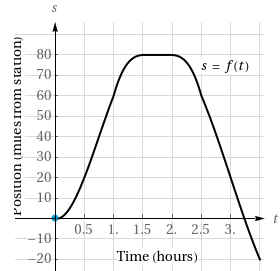
\includegraphics[width=0.85\linewidth]{srcImages/fig3-40}
  \end{flushright}
\end{minipage}

\pagebreak
\begin{defn*}[Velocity, Speed, and Acceleration]
  Suppose an object moves along a line with position $s=f(t)$. Then
    \begin{center}
      \def\arraystretch{2}
      \begin{tabular}{@{}lR@{\ =\ }L@{}}
        the \textbf{velocity} at time $t$ is& v& \dfrac{ds}{dt}=f'(t)\\
        the \textbf{speed} at time $t$ is & \abs{v}&\abs{f'(t)}, \text{ and}\\
        the \textbf{acceleration} at time $t$ is & a&\dfrac{dv}{dt}=\dfrac{d^2s}{dt^2}=f''(t).
      \end{tabular}
    \end{center}
\end{defn*}
\noindent
\begin{minipage}[t]{0.6\linewidth}~
  \begin{itemize}
    \item Velocity indicates direction: 
    
    \hfill forward is positive, backward is negative
    \item Speed is direction independent:
    
    \hfill $v(t)=-30 m/s \Rightarrow \textnormal{speed }=30 m/s$.
    \item If displacement changes signs, then velocity was zero.
    
    A velocity of zero does not indicate a change in direction.
  \end{itemize}
\end{minipage}%
\begin{minipage}[t]{0.4\linewidth}~

  \begin{flushright}
    \begin{tikzpicture}
      \begin{axis}[
        axis lines=center,
        axis line style={->},
        xmin=-0.5, xmax=5.0,
        ymin=-7.5, ymax=22.5,
        xtick={-4,1,...,6},
        ytick={-5,5,...,25},
        minor x tick num=3,
        minor y tick num=1,
        ticklabel style={font=\footnotesize,inner sep=0.5pt,fill=white,opacity=1.0, text opacity=1},
        %xlabel=$x$, xlabel style={at={(ticklabel* cs:1)},anchor=north west},
        %ylabel=$y$, ylabel style={at={(ticklabel* cs:1)},anchor=south west},
        every axis plot/.append style={line width=0.95pt}
        ]
        \addplot[-] expression[domain=0:5, ClemsonOrange, samples=100] {x^3-6*x^2+9*x}
          node[above, black, pos=0.15] {$s$};
        \addplot[-] expression[domain=0:5, ClemsonPurple, samples=100] {3*x^2-12*x+9}
          node[right, black, pos=0.025] {$v$};
        \addplot[-] expression[domain=0:5, black, opacity=0.60, samples=2, text opacity=1] {6*x-12}
          node[above, black, pos=0.65] {$a$};
      \end{axis}
    \end{tikzpicture}
  \end{flushright}
\end{minipage}%

\pagebreak
\begin{ex*}
  $s=-t^3+3t^2-3t,\ 0\leq t\leq 3$ gives the position $s=f(t)$ of a body moving on a coordinate line, with $s$ in meters and $t$ in seconds.
  \begin{enumerate}
    \item Find the body's displacement and average velocity for the given time interval.
    \item Find the body's speed and acceleration at the endpoints of the interval.
    \item When, if ever, during the interval does the body change direction?
  \end{enumerate}
\end{ex*}

\pagebreak
\noindent
For vertical motion (e.g. an object thrown up in the air), an object's maximum height occurs when velocity is zero and hits the ground at height zero.
\begin{ex*}
  A rock is thrown vertically upward from the surface of the moon at a velocity of 24 m/sec (about 86 km/h) reaches a height of $s=24t-0.8t^2$ meters in $t$ sec.
  \begin{enumerate}
    \item Find the rock's velocity and acceleration at time $t$. (The acceleration in this case is the acceleration of gravity on the moon.)
    \item How long does it take for the rock to reach it's highest point?
    \item How high does the rock go?
    \item When does the rock hit the ground?
    \item What is the velocity at that instant?
  \end{enumerate}
\end{ex*}

\pagebreak
\begin{ex*}
  Suppose a stone is thrown vertically upward from the edge of a cliff on Earth with an initial velocity of 32 ft/s from a height of 48 ft above the ground. The height (in feet) of the stone above the ground $t$ seconds after it is thrown is $s(t)=-16t^2+32t+48$.
  \begin{enumerate}
    \item Determine the velocity $v$ of the stone after $t$ seconds.
    \item When does the stone reach its highest point?
    \item What is the height of the stone at the highest point?
    \item When does the stone strike the ground?
    \item With what velocity does the stone strike the ground?
    \item On what intervals is the speed increasing?
  \end{enumerate}
\end{ex*}

\pagebreak
\begin{ex*}[Velocity of a bullet]
  A bullet is fired vertically into the air at an initial velocity of 1200 ft/s. On Mars, the height $s$ (in feet) of the bullet above the ground after $t$ seconds is $1200t-6t^2$ and on Earth, $s=1200t-16t^2$. How much higher will the bullet travel on Mars than on Earth?
\end{ex*}

\pagebreak
\begin{defn*}[Average and Marginal Cost]
  The \textbf{cost function} $C(x)$ gives the cost to produce the first $x$ items in a manufacturing process. The \textbf{average cost} to produce $x$ items is $\bar C(x)=C(x)/x$. The \textbf{marginal cost} $C'(x)$ is the approximate cost to produce one additional item after producing $x$ items.
\end{defn*}
\begin{ex*}
  Suppose $C(x)=10,000+5x+0.01x^2$ dollars is the estimated cost of producing $x$ items. The marginal cost at the production level of 500 items is:
\end{ex*}
\vspace*{\stretch{1}}

\begin{ex*}
  The cost function for production of a commodity is
    $$C(x)=339+25x-0.09x^2+0.0004x^3$$
  \begin{enumerate}
    \item Find and interpret $C'(100)$.
    \item Compare $C'(100)$ with the cost of producing the 101st item.
  \end{enumerate}
\end{ex*}

\vspace*{\stretch{1}}
\pagebreak

\begin{ex*}
  For the following cost functions,
  \begin{enumerate}[label=\alph*)]
    \item Find the average cost and marginal cost functions.
    \item Determine the average cost and the marginal cost when $x=a$.
    \item Interpret the values obtained in part (b)
  \end{enumerate}
  \begin{enumerate}[itemsep=\stretch{1}]
    \item $C(x)=500+0.02x,\ 0\leq x\leq 2000,\ a=1000$.
    \item $C(x)=-0.01x^2+40x+100,\ 0\leq x\leq 1500,\ a=1000$.
  \end{enumerate}
  \vspace*{\stretch{1}}
\end{ex*}

\pagebreak
\end{document}

  \documentclass[../mathNotesPreamble]{subfiles}
\begin{document}
%\relscale{1.4}
\section{JIT 12.1: Decomposition of Functions}
\begin{ex*}
  Decompose the following functions:
\end{ex*}
\begin{enumerate}
  \item A function under a power
    \begin{tasks}(3)
      \task $y(x)=\parens{x^3-1}^2$
      \task $y(x)=\parens{\sqrt[5]{x}-1}^\frac{2}{3}$
      \task $y(x)=\tan^2(x)$
    \end{tasks}
    \vspace*{\stretch{1}}
  \item The argument of a trig function
    \begin{tasks}(3)
      \task $y(x)=\cos\parens{x^5}$
      \task $y(x)=\sin\sqrt x$
      \task $y(x)=\sin\parens{3^x}$
    \end{tasks}
    \vspace*{\stretch{1}}
  \item The functional power of an exponent
    \begin{tasks}(1)
      \task $y(x)=e^{3x+1}$
    \end{tasks}
    \vspace*{\stretch{1}}
  \item Various combinations
    \begin{tasks}(3)
      \task $y(x)=\tan^3\parens{2x}$
      \task $y(x)=2^{\sqrt{\sin(x)}}$
      \task $y(x)=\cos\parens{x^3-2}^{\sfrac{2}{7}}$
    \end{tasks}
\end{enumerate}
\vspace*{\stretch{1}}
\pagebreak

\end{document}

  \documentclass[answers]{exam}
\usepackage{texPreamble}
\usepackage{relsize}
\usepackage{tabularx}
\extraheadheight{0.25in}
\extrafootheight{1.0in}
\extrawidth{1in}
% ----------------------------------------------------------------
\firstpagefootrule
\runningfootrule
\begin{document}
%\relscale{1.4}
\section{3.7: The Chain Rule}
\begin{center}
  \fbox{\parbox{0.95\linewidth}{
    \textbf{Theorem 3.13} The Chain Rule
    
    Suppose $y=f(u)$ is differentiable at $u=g(x)$ and $u=g(x)$ is differentiable at $x$. The composite function $y=f(g(x))$ is differentiable at $x$, and its derivative can be expressed in two equivalent ways.
      \begin{align}
        &\dfrac{dy}{dx} = \dfrac{dy}{du}\cdot \dfrac{du}{dx}\\[10pt]
        &\dfrac{d}{dx}\parens{f\parens{g(x)}}=f'\parens{g(x)}\cdot g'(x)
      \end{align}
  }}
\end{center}
\begin{ex*}
  Take the derivatives of the following functions
\end{ex*}
\begin{tasks}[after-item-skip=\stretch{1}](2)
  \task $y=\parens{3x^3+1}^2$
  \task $y=\parens{3x^3+1}^7$
  \task $y=6\cos^2(x)$
  \task $y=\sin\parens{x+\cot(x)}$
\end{tasks}
\vspace*{\stretch{1}}
\begin{center}
  \fbox{\parbox{0.95\linewidth}{
    To use the chain rule,
    \begin{itemize}
      \item Identify the inner and outer function
      \item Take the derivative of the outside, leaving the original inner function
      \item Multiply by the derivative of the inner function
    \end{itemize}
  }}
\end{center}
\pagebreak

\begin{tasks}[resume, after-item-skip=\stretch{1}](2)
  \task $y(x)=e\inv[4x]$
  \task $y(x)=\parens{\dfrac{x-2}{2x+1}}^9$
  \task $y(x)=\sqrt{\sec(x)}$
  \task $y(x)=2\parens{8x-1}^3$
  \task $y(x)=\parens{\frac{x}{2}-1}\inv[10]$
  \task $y(t)=e^{\sin(t)}+\sin(e^t)$
\end{tasks}
\vspace*{\stretch{1}}
\pagebreak

\begin{tasks}[resume, after-item-skip=\stretch{1}](2)
  \task $y(x)=x^2 e^{x^2}$
  \task $\dfrac{f(x)}{g(x)}=f(x)\cdot\sbrkt{g(x)}\inv$
  \task $y(x)=f\parens{g\parens{h(x)}}$
  \task $y(x)=-12e^{3x^7}$
  \task* $y(x)=\dfrac{\cos^2(x)}{e^x\parens{x^2+4}}$
  
\end{tasks}
\vspace*{\stretch{1}}
\pagebreak

\end{document}

\end{document}
